%%%%%%%%%%%%%%%%%%%%%%%%%%%%%%%%%%%%%%%%%%%%%%%%%%%%%%%%%%%%%%%%%%%%%%%%%%%%%%%
%%	PARA INSERTAR FIGURAS USAR LA FUNCION PREDEFINIDA \imagen
%%
%%      \imagen{escala}{path imagen}{caption}{referencia}
%%
%% donde:
%% 	* escala: es un valor numérico. Preferentemente usar valores entre 0 y 1.
%%		(ejemplo: 0.2)
%% 	* path: imagen es el directorio relativo donde se encuentra la imagengit
%%		(ejemplo: Figures/Logos/conae-logo.png)
%%	* caption: texto de pie de figura.
%%	* referencia: texto que sirve para citar la figura.
%%		(ejemplo: fig:conaelogo) luego se podrá hacer referencia \ref{fig:conaelogo}
%%%%%%%%%%%%%%%%%%%%%%%%%%%%%%%%%%%%%%%%%%%%%%%%%%%%%%%%%%%%%%%%%%%%%%%%%%%%%%%

%------------------------------------------------------------------------------
% Formato del documento
\documentclass[11pt, a4paper, twoside]{report}

%------------------------------------------------------------------------------
% TEMPLATE MDIAE (ACÁ SE ENCUETRAN LAS CUSTOMIZACIONES)
% Remitirse al archivo mdiaedoc.sty
\usepackage{mdiaedoc}

%Configuración de los márgenes
\usepackage[top=3cm, bottom=3cm, left=2.5cm, right=1.5cm]{geometry}

\usepackage{natbib}
\usepackage{import}

% Para gráficos
\usepackage{tikz}
\usetikzlibrary{shapes,snakes}
\usetikzlibrary{arrows,positioning}
\usetikzlibrary{babel}

%Para agregar notas
\usepackage{todonotes}

% For comment
\usepackage{comment}

% For appendix
\usepackage{appendix}

% For epigraph
\usepackage{epigraph}

% For rotate image
\usepackage{rotating}

%------------------------------------------------------------------------------
% Esto no se usa (YA ESTA DEFINIDO EN EL TEMPLATE)
%\usepackage{setspace}

%%%%%%%%%%%%%%%%%%%%%%%%%%%%%%%%%%%%%%%%%%%%%%%%%%%%%%%%%%%%%%%%%%%%%%%%%%%%%%%
% COMIENZO DEL DOCUMENTO
%%%%%%%%%%%%%%%%%%%%%%%%%%%%%%%%%%%%%%%%%%%%%%%%%%%%%%%%%%%%%%%%%%%%%%%%%%%%%%%
\begin{document}

\makeatletter
\author{Arias Emmanuel}
\makeatother

%------------------------------------------------------------------------------
% PORTADA
\portadatesis{Diseño de una arquitectura de aviónica tolerante a fallas basada en componentes COTS para vehículos
satelitales de nueva generación}{Arias Emmanuel}{UNIVERSIDAD NACIONAL DEL CÓRDOBA}{Mayo,
2017}{2017}{Gustavo Wiman}{INVAP, Bariloche, Provincia de Rio Negro}

%------------------------------------------------------------------------------
% EN CASO DE TENER UN ASESOR CIENTIFICO, DESCOMENTAR LO SIGUIENTE
% \begin{center}
% \normalsize ASESOR CIENTÍFICO:\\
% \normalsize \textit{\textbf{Nombre del asesor}}\\
% \end{center}

%------------------------------------------------------------------------------
% COMPLETAR CON LICENCIA CREATIVE COMMONS SEGÚN CORRESPONDA
%\begin{center}
%%%%% Ejemplo %%%%%%
%\begin{figure}[H]
%    \centering
%    
\includegraphics[width=3cm, keepaspectratio=true]{imagenes/Logos/creativecommons.png}
%\end{figure}
%\vspace*{-0.5cm}
%Esta obra está bajo una \href{http://creativecommons.org/licenses/by-sa/2.5/ar/}{Licencia Creative Commons Atribución-CompartirIgual 2.5 Argentina.}
%\end{center}

\pagenumbering{gobble}


\thispagestyle{empty}

\vspace*{4cm}
\hfill\normalsize\textit{\sf A mis padres}
\chapter*{Abstract}
\label{chap:abstract}

\textbf{Keywords:}
\chapter*{Resumen} % si no queremos que añada la palabra "Capitulo"
%\addcontentsline{toc}{chapter}{Resumen} % si queremos que aparezca en el índice

Esta tesis se trata de
\chapter*{Agradecimientos}
\label{chap:agradecimientos}
%\addcontentsline{toc}{chapter}{Agradecimientos}
En primer lugar, me gustaría agradecer a mi madre, que gracias a sus palabras de aliento, 
que me han acompañado en la distancia y a lo largo de estos dos años, hoy puedo estar
concretando esta meta. Sinceramente, si no fuese por ella, hoy estaría persiguiendo
otros objetivos. Desde chiquito me ha inculcado a que nunca debo bajar los brazos,
aún cuando todo parezca que está perdido. Siempre hay que luchar hasta el final.
Es por eso que hoy estoy aquí. Gracias mamá.

En segundo lugar, quiero agradecer a mi novia la Prof. Dra. Bioq. Brandán Yamila por su
comprensión, su compañía, su cariño, su amor y sus consejos. Además, quisiera agradecer y destacar
enormemente, que debido a su gran experiencia en el área de la investigación,
ha sabido guiarme y ayudarme en el desarrollo de esta tesis. Gracias amor. 

Por último lugar, quisiera agradecer a mis compañeros de maestría, Alfonso, Cecilia,
Eduardo, Elbio, Ezequiel, Javier, José, Pablo E., Pablo S. y Ricardo, por su amistad y
por compartir sus conocimientos. Gracias.



 %% OPCIONAL

\tabladecontenidos

\chapter*{Lista de acrónimos}
\label{chap:acronimos}
\begin{acronym}[TESIS]
\acro{SW}{Software}
\acro{HW}{Hardware}
\acro{FT}{Tolerancia a Fallas}
\acro{FA}{Evitación de Fallas}
\acro{FR}{Eliminación de Fallas}
\acro{FF}{Predicción de Fallas}
\acro{MTBF}{Tiempo Medio Entre Fallas}
\acro{MTTF}{Tiempo Medio de Fallas}
\acro{MTTR}{Tiempo Medio de Reperación}
\acro{CMF}{Modo Común de fallas}
\acro{FDIR}{Detección, Aislación y Recuperación de Fallas}
\acro{CONAE}{Comisión Nacional de Actividades Espaciales}
\acro{UNLAM}{Universidad Nacional de La Matanza}
\acro{INVAP}{Investigación Aplicada}
\acro{NASA}{National Aeronautics and Space Administration}
\acro{COTS}{Commercial Off-The-Shelf}
\acro{TT}{Time-Trigged}
\end{acronym}


%-------------------------------------------------------------------------------
%TODO: Elminiar esta tabla antes de enviar a corregir
%-------------------------------------------------------------------------------
\listoftodos


%------------------------------------------------------------------------------
% Numeración arábiga a partir de este punto
\chapter{Introducción}\label{chap:intro}
% TODO: Introuducción, extraída desde el plan de tesis,
En el marco del Plan Espacial Nacional, desarrollado por la \ac{CONAE} de Argentina, y con el propósito de llevar a cabo actividades de investigación y 
aplicación, provenientes de la \ac{UNLAM} se presenta este plan de tesis con el fin de ampliar los 
conocimientos y la participación de la \ac{CONAE} y \ac{UNLAM}, en el campo del Desarrollo Informático y 
Ciencias de la Computación.

Las actividades desarrolladas para este trabajo de tesis son realizadas, en su mayor proporción, en 
la Unidad de Desarrollo \ac{INVAP}, ubicada en San Carlos de Bariloche, Provincia de Río Negro. Este 
trabajo se encuentra orientado a brindar un nuevo conocimiento, que ayude en cierta medida, en el 
desarrollo de los diferentes proyectos con los que cuenta actualmente esta empresa, agregando un 
grado de innovación en el resultado que se obtenga.

\ac{INVAP} tiene como visión ser un referente en proyectos tecnológicos a nivel mundial \cite{invapWEB}, 
por lo tanto, debe asegurarse que cada uno de los productos que se lleven a cabo sean competitivos. 
Para lograr cumplir con esto, es necesario que tales proyectos se encuentren a la vanguardia 
tecnológica y científica.  

El desarrollo de proyectos satelitales conlleva costos de importante magnitud, y 
dependen de cada misión. Una parte importante de los costos está conformado por el 
desarrollo\footnote{\textit{Nota: entiéndase por desarrollo al proceso de planificación, análisis, 
diseño e implementación.}} y sobre todo los materiales que se utilizan para su fabricación. Esto 
es debido a que se utilizan componentes que son exclusivos para el ámbito espacial, en otras 
palabras que se encuentran ``calificados para volar''. Estos componentes son fabricados especialmente para soportar el ambiente hostil del espacio.

Si se considera al ámbito espacial como una industria, algo que ha sido demostrado en los últimos 
años; y si se tiene en cuenta las intenciones de crecimiento y competitividad de la empresa INVAP,  de permitir el ingreso de nuestro pais en el mercado satelital \cite{invapWEB}, resulta de gran 
importancia lograr reducir los costos en fabricación y desarrollo de vehículos satelitales.

La \ac{NASA} tiene un enfoque de desarrollo bajo el lema 
``faster, cheaper, better'' \cite{Forsberg99}, lo cual busca desarrollar sus proyectos y misiones 
de foma rápida, barata y mejor. Bajo este enfoque se han realizado diversos estudios e 
investigaciones dando resultados sumamente positivos \cite{Tai99}, \cite{Chau99}, 
\cite{Schneidewind98}, \cite{Forsberg99}. En estos trabajos se utilizan componentes que no se 
encuentran ``calificados para volar'',  los cuales también son llamados componentes \ac{COTS}, o de estantería. Debe mencionarse, que también hubo algunos 
fracasos en su aplicación. 

A simple vista, la utilización de estos componentes ayudaría a reducir costos. Sin embargo, esto 
no es tan directo. Los componentes \ac{COTS} al no estar calificados, se les deben realizar tareas 
de calificación adicional. Además deben ser aplicados a un ambiente, que asegure 
que no fallarán durante la misión; o si fallan, no será motivo de pérdida de la misma. 

Los componentes \ac{COTS} suelen tener un costo de compra entre 100 y 1000 veces menores que aquellos 
que está califcados para volar. Por lo que el aumento en la utilización de estos componentes, 
aplicados al desarrollo de diferentes tipos de satélite, \textbf{permitiría reducir los costos y 
ahorrar algunos millones de dólares del proyecto satelital.} Esto facilitaría el ingreso de 
Argentina en un mercado altamente competitivo.

El desafío de este trabajo de tesis es analizar y estudiar arquitecturas que sean tolerantes a 
fallas, que permitan una correcta comunicación entre los diferentes subsistemas de un vehículo 
espacial de nueva generación, y que tenga como característica principal un cierto grado de confiabilidad, de modo tal que pueda ser aplicado con componentes \ac{COTS}.

\section{Motivación}\label{chap:motivacion}
Los costos de un proyecto satelital se pueden clasificar, a grandes rasgos, en 5 grupos:
\begin{itemize}
 \item Desarrollo
 \item Materiales
 \item Ensamblado, integración, y tests
 \item Lanzamiento
 \item Operaciones
\end{itemize}

Este trabajo de tesis se centrará principalmente en el desarrollo (proceso de planificación, 
análisis, diseño e implementación.), y en los materiales utilizados en la fabricación de vehículos satelitales.

No se puede mencionar a ciencia cierta cuál es el costo “verdadero” de desarrollar un satélite. Este 
depende exclusivamente del tipo de satélite y de la misión. Lo que si se debe tener en claro es que 
las tareas de desarrollo representan una parte muy importante del costo total del proyecto.

Desarrollar un vehículo espacial con componente \ac{COTS}, en un principio podría representar costos 
adicionales, ya que se le deben realizar tareas de calificación adicional, debido a que no están 
“preparados” para resistir las condiciones hostiles del espacio. 

Uno de los puntos positivos, y que motivan la aplicación de componentes COTS, es que a la hora de 
desarrollar varios satélites en base a la misma ingeniería, se puede ahorrar en gran medida en los 
materiales que se utilizan. Los componentes \ac{COTS} suelen tener un costo de compra entre 100 y 1000 
veces menores que aquellos que están calificados para volar. \textbf{Esto ayudaría a ahorrar 
algunos millones de dólares de los proyectos satelitales.}
  
Otra de las ventajas de utilizar componentes \ac{COTS}, es que la mayoría cuentan con una tecnología más 
avanzada que aquellos que son calificados para volar. Esta tecnología permite:
\begin{itemize}
 \item Aumentar prestaciones, mediante el incremento de las capacidades de procesamiento, memoria, 
velocidades de 
procesamiento, etc.
 \item Implementar funciones que son imposibles de aplicar en tecnologías viejas.
 \item Reducir tiempos de desarrollo.
 \item Reducir volumen, masa y consumo
\end{itemize}

El último punto mencionado anteriormente es de especial interés, ya que al reducir volumen y masa, 
permite reducir costos adicionales como el de lanzamiento.

Esta reducción de costos de proyectos satelitales tienen ventajas directas a la hora de introducir a 
Argentina en un mercado altamente competitivo, donde la mínima reducción de estos, representa 
ganancias económicas importantes. 
 
Uno de los puntos en contra de la utilización de componentes \ac{COTS} es que al no ser calificados para 
volar, es necesario llevar a cabo tareas y estrategias inteligentes, con el fin de hacer frente a 
esa “deficiencia”. Por ello, se exige realizar una investigación y análisis de diferentes 
arquitecturas de aviónica, que puedan ser utilizadas para lograr que el sistema sea tolerante a 
fallas, y así, cumplir con los requerimientos de una misión satelital. 

El estudio de arquitecturas tolerantes a fallas, no solamente tiene aplicación en el ámbito 
espacial, si no que también puede ser extendido a cualquier sistema crítico, los cuales necesitan 
ser robustos y tolerantes a fallas, como es el caso de aviones comerciales, plantas nucleares, 
automóviles, etc.

% --------------------- %
% TODO: Hipótesis
% --------------------- %
\section{Hipótesis}
La hipótesis de esta tesis es la siguiente: ``Una arquitectura de aviónica  basadas en componentes 
\ac{COTS}, robusta y tolerante a fallas, es totalmente aplicable y utilizable en vehículos espaciales, 
con un alto nivel de confiabilidad, lo cual permite disminuir la complejidad de los sistemas actuales de aviónica''.

\section{Objetivo del trabajo y preguntas de investigación}

\subsection{Objetivo}
El objetivo de este trabajo es investigar y analizar arquitecturas de comunicación de los 
subsistemas de aviónica tolerante a fallas basada en componentes \ac{COTS} para vehículos 
satelitales de nueva generación.

% secondary objectives
\subsection{Objetivos Específicos}
\begin{enumerate}
 \item Realizar un estudio del estado de la cuestión sobre arquitecturas tolerantes a fallas para 
sistemas críticos.
 \item Investigar y analizar arquitecturas tolerantes a fallas que aseguren la confiabilidad del 
sistema y que sean aplicables en la industria satelital.
 \item Investigar y analizar protocolos de comunicación, para las capas superiores del modelo de 
OSI (modelo de interconexión de sistemas abiertos - ISO/IEC 7498-1), orientados a la tolerancia a 
fallas y confiabilidad de los sistemas. Realizar un estudio comparativo de los diferentes 
protocolos estudiados.
 \item Investigar una metodología para lograr una medición de la tolerancia a fallas en 
arquitecturas de aviónica.
 \item Desarrollar un estudio comparativo de arquitecturas tolerantes a fallas con el fin de obtener 
ventajas y desventajas de cada una de ellas.
 \item Diseñar modelos alternativos de arquitecturas tolerantes a fallas, que tenga un grado de 
confiabilidad tal que permita la aplicación de componentes \ac{COTS}.
 \item Evaluar la confiabilidad de los modelos de arquitecturas (mediante métrica desarrollada en 
este trabajo o siguiendo otras estrategias). 
 \item Proponer el diseño de una nueva arquitectura tolerante a fallas, con un 
grado de confiabilidad suficiente para la aplicación de componentes \ac{COTS} en aviónicas de vehículos 
satelitales.
\item Simular la arquitectura planteada para medir su grado de tolerancia a fallas y perfomance.
\end{enumerate}

\pagenumbering{arabic}
\setcounter{page}{1}

% Marco Teorico
\chapter{Marco Teórico}\label{chap:marco_teorico}
\epigraph{I recall seeing a package to make quotes}{Snowball}
% section that talk about terminology
% esta seccion habla sobre los términos importantes a utilizar a lo largo de la tesis
\section{Terminología}\label{sec:terminologia}
Existe una importante diferencia entre los significados de las palabras falla, error y
avería\footnote{En inglés: fault, error y failure.}, que es importante destacar antes de comenzar
con el desarrollo de este trabajo.

Un \textbf{avería} de sistema ocurre cuando el servicio prestado por el sistema ya no coincide con
las especificaciones del mismo \citep{Hanmer07}. Esto quiere decir que existe un problema que tiene
una consecuencia negativa en el sistema completo, logrando que este ya no logre cumplir con sus
especificaciones. Cuando el sistema no se comporta de la manera que es especificada, este ha
fracasado. Esto significa que lo que se espera de un sistema se encuentra descripto, comúnmente en
especificaciones o requerimientos \citep{Pullum01}.

Para la \cite{IEEE610.12} avería es ``la inhabilitación de una sistema o componente a llevar a
cabo las funciones requeridas en los requerimientos específicos de perfomance del mismo''.

\cite{Hanmer07} ejemplifica averías de sistemas cuando: el sistema se bloquea y se detiene cuando no
debería hacerlo, el sistema calcula un resultado incorrecto, el sistema no está disponible, el
sistema es incapaz de responder a la interacción con el usuario. Cuando el sistema no hace lo que
debe hacer, el sistema ha fracasado. Las averías son detectados por los usuarios mientras usan el
sistema.

Las averías son causados por los errores. Un \textbf{error} es una parte del estado del sistema
que es susceptible de provocar un avería en el sistema, un error que afecta al servicio es una
indicación de que un avería se ha producido \citep{Hanmer07}. Un error se puede propagar, es decir
dar a lugar otros errores \citep{Pullum01}.

\cite{IEEE610.12} define error como ``la diferencia entre un valor computado, observado o medido,
con el valor verdadero, especificado o el teóricamente verdadero''.

Los errores se pueden clasificar en dos tipos: errores de tiempo y valores \citep{Hanmer07}. Los
errores de valores son aquellos que se manifiestan como valores discretos incorrectos o estados del
sistema incorrecto. En cambio, los errores de tiempo pueden incluir aquellos que no cumplen con el total de las tareas.

\cite{Hanmer07} especifica los siguiente casos más comunes de errores:
\begin{itemize}
 \item Timing: existe una falta de sincronización en la comunicación de los procesos.
 \item Bucles infinitos: ejecución de un bucle sin detenerse, esto consume memoria, y la
avería del sistema.
 \item Error de protocolo: errores en el flujo de comunicación ya que no coinciden los
protocolos. Mensajes enviados en formato diferente, en tiempos diferentes, a lugares de sistemas
incorrectos.
 \item Inconsistencia de datos: errores son diferentes en diferentes lugares.
 \item Sobrecarga de sistema: el sistema es incapaz de hacer frente a la sobrecarga de
actividades a la que es expuesta.
\end{itemize}

La causa adjudicada o la hipótesis de un error es una \textbf{falla}, también llamado ``bugs''. Una
\textbf{falla activa} es aquella que produce un error \citep{Pullum01}. Una falla es un defecto que está
presente en el sistema y que puede causar un error \citep{Hanmer07}. Es la desviación actual de lo
correcto \cite{Hanmer07}.

Según \cite{IEEE610.12} una falla es ``un defecto en un dispositivo de hardware o componente; como
por ejemplo un corto circuito o un cable cortado''. También realiza una segunda definición diciendo
que falla es ``un paso incorrecto, proceso, o definición de dato en un programa de computadora''
\cite{IEEE610.12}. Esta última afirmación es la que se usa en el ámbito de este trabajo.

Algunas fallas introducidas en el \ac{SW} se detallan en \cite{Hanmer07}, lo cual señala que
pueden incluir:
\begin{itemize}
 \item Especificaciones incorrecta de requerimientos
 \item Diseño incorrecto
 \item Errores de programación
\end{itemize}

Entonces, como lo indica \cite{Pullum01} con la tolerancia a fallas, lo que se busca es prevenir la
avería mediante la ``tolerancia'' de fallas, las cuales son detectables cuando un error aparece.
Las fallas son el motivo de errores y los errores son motivos de avería \citep{FTDesign}.

También se suele utilizar el término anomalía en las operaciones de vehículos espaciales para
referirse a comportamientos anómalos o no esperados del sistema \citep{SpaceSystemFailures}

En \cite{FTDesign} se describe un ejemplo para diferenciar correctamente estos conceptos. Se considera
el \ac{SW} de una planta nuclear, en la cual existe una computadora que es responsable de controlar
la temperatura, la presión y demás variables de interés para la seguridad del sistema. Se da el
caso de que uno de los sensores detecta que la turbina principal se encuentra girando a una
velocidad menor a la correcta. Esta falla hace que el sistema envíe una señal para aumentar su
velocidad (error). Esto produce un exceso de velocidad en la turbina, lo cual tiene como
consecuencia que la seguridad mecánica apague la turbina. En esta situación el sistema no está
generando energía. Esto se considera un avería, porque el sistema no está entregando el servicio
según lo establecido por los requerimientos. Pero es un avería salvable.

Otro concepto es el de \textbf{mantenibilidad}, este es la capacidad de un sistema, bajo condiciones normales, de ser restaurado a un estado en el cual puede realizar sus funciones requeridas, cuando se realiza el mantenimiento \citep{Rausand04}.

En secciones posteriores se ven los conceptos de confiabilidad, disponibilidad y seguridad (Sección \ref{subsec:confiabilidad}, \ref{subsec:disponibilidad}, \ref{subsec:seguridad}, respectivamente).


% Section that talk about dependability on software
% TODO:La fiabilidad en el software
\section{La fiabilidad en el software}\label{sec:fiabilidad_software}
El objetivo final de la \ac{FT}, es el desarrollo de un sistema fiable \citep{FTDesign}. Teniendo
en cuenta que \ac{SW} que se encuentra dentro de las naves espaciales, como satélites,
lanzadores, y sobre todo vehículos tripulados son críticos, ya que de ellos dependen el éxito o
fracaso de una misión o la vida de seres humanos,y se debe llevar a cabo un sistema fiable.
La fiabilidad de un sistema es la capacidad del mismo de entregar a los usuarios un nivel
deseado de servicio \citep{FTDesign}.

La fiabilidad también se la puede considerar como una propiedad global que permite justificar la
confianza de los servicios de un sistema \citep{FTAvionics}. Por lo tanto, como lo indica
\cite{FTAvionics} la fiabilidad es un término amplio y cualitativo que está relacionado con
atributos no funcionales (o ``-ilities''), que buscan generar un sistema ``ideal'', especialmente
cuando su funcionamiento es crítico.

Como se muestra en la Figura \ref{fig:dependability_relations} la consecuencia de la fiabilidad es
la relación entre la evitación de fallos y la reducción de fallos, así como también la \ac{FT}.

\begin{figure}[h]
 \centering
 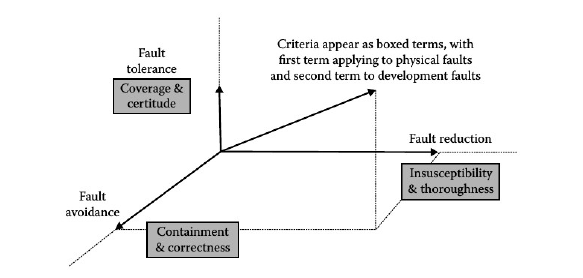
\includegraphics[scale=0.5]{images/Marco_teorico/dependability_relations}
  \caption{Fiabilidad \protect\citep{FTAvionics}}
\label{fig:dependability_relations}
\end{figure}

Según \cite{Pullum01} la fiabilidad puede ser clasificada en:
\begin{itemize}
 \item Impedimentos: son aquellas cosas que se interponen en el camino de la fiabilidad. Son las
fallas, errores y fracasos.
 \item Medios: los medios para lograr la fiabilidad, según el autor, se pueden dividir en dos
grupos:
  \begin{enumerate}
    \item Aquellos que son utilizados durante la construcción del \ac{SW} (\ac{FA}\footnote{En
    inglés, Fault Avoidance} y \ac{FT}).
    \item Aquellos que contribuyen con la validación del \ac{SW} una vez desarrollado
    (\ac{FR}\footnote{En inglés, Fault Removal} y \ac{FF}\footnote{En inglés, Fault Forecasting}).
  \end{enumerate}

 \item Atributos: describen las propiedades de la fiabilidad y proporcionan una forma de evaluar el
logro de esas propiedades.
\end{itemize}

% TODO: deteriodo de la confiabilidad
\section{Impedimentos de la confiabilidad}\label{sec:impedimentos}
El impedimiento de la confiabilidad o deterioro de la confiabilidad es definido en términos de
fallas, errores, y fracaso \citep{FTDesign}. Los mismos fueron desarrollados en la sección
\ref{sec:terminologia}. Lo que tienen en común estos tres conceptos, es que avisan, o dan alerta
cuando algo está mal \citep{FTDesign}. La diferencia radica, en que las fallas son a nivel físico;
los errores se dan a nivel computacional; mientras que los fracaso se dan a nivel de sistema
\cite{FTDesign}.

\subsection{Orígenes de la falla}
Existen diversos orígenes de fallas. Estas pueden provenir desde terceros, en el caso de productos
comprados, pueden deverse a una falta del conocimiento del problema, falta de tiempo, etc.
\cite{FTDesign} clasifica el orígen de las fallas en cuatro grupos: \textit{especificación
incorrecta, implementación incorrecta, defectos de fabricación y factores externos}

Las \textit{especificaciones incorrectas} son aquellas que surgen debidas a una incorrecta
especificación de requerimiento o un mal diseño de una arquitectura o de un algoritmo
\citep{FTDesign}. Estos orígenes de fallas son bastante comúnes en el desarrollo de sistemas. Un
ejemplo típico citado por \cite{FTDesign}, es el caso de requerimientos que ignoran aspectos del
medio ambiente en el que opera el sistema. Una mala redacción de un requerimiento o el olvido de
uno de ellos, puede traer graves problemas, atrasos y pérdida de dinero,  en el diseño y producción
de un sistema espacial.

Las \textit{implementaciones incorrectas}, se refieren a las \textit{fallas de diseño}, surgen
cuando el sistema implementado no cumple con los requerimientos \citep{FTDesign}.

Otro orígen de falla son los \textit{defectos de los componentes} \citep{FTDesign}.Estos pueden
incluir defectos de fabricación, defectos aleatorios dados en los componentes, etc.

Y por último se tienen las fallas que son causadas por \textit{factores externos}, los cuales
provienen del medio ambiente, usuarios u operadores \citep{FTDesign}. Ejemplos de estos factores
externos pueden ser, vibraciones, cargas electroestáticas, temperatura, radición electromagnética,
envío incorrecto de comandos, etc.

% TODO: Modos comúnes de fallas
\subsection{Modos comúnes de fallas}
Un \textit{\ac{CMF}}\footnote{En inglés, common-mode faults} es una falla que ocurre
simultaneamente en dos o más componentes redundantes \citep{FTDesign}.

\cite{Gangloff75} define los \ac{CMF} como múltiples unidades de fracaso debido a una sola causa.

\ac{CMF} son causados por fenómenos que crean dependencias entre unidades redundadas, lo que causa
la falla de estas unidades simultaneamente \citep{FTDesign}.

Según como lo indica \cite{FTDesign} el único enfoque para combatir los \ac{CMF}, es mediante el
diseño en diversidad. Diseño en diversidad es la implementación de más de una variante de la
función en cuestión \citep{FTDesign}. Esto se puede lograr variando los algoritmos que se utilizan,
diferentes equipos de trabajo realicen las mismas partes del sistema, de manera tal de tener
redundancia en código, etc.

%TODO: Fallas en el Software
\subsection{Fallas en el Software}
El \ac{SW} difiere en gran medida con el \ac{HW}. En primer lugar el \ac{SW} no envejece, no se deforma, tampoco se puede quebrar ni ser afectado
por el medio ambiente. El \ac{SW} es determinístico, siempre responde de la misma manera en el mismo ambiente, al menos que falle.

Por otro lado el \ac{SW} se lo puede actualizar varias veces a lo largo del su ciclo de vida.

En tercer lugar, arreglar bugs de \ac{SW} \textbf{no significa que el mismo sea más confiable}, al contrario pueden ocurrir nuevos errores \citep{FTDesign}.

Por último el \ac{SW} es mucho más complejo y menos regular que el \ac{HW}. Tests tradicionales y métodos de debug pueden ser inadecuados para los sistemas de \ac{SW}

% TODO: medios de fiabilidad
\section{Medios de fiabilidad}\label{sec:medios_falla}
Los medios de confiabilidad son métodos y técnicas que permiten el desarrollo de un sistema
confiable \citep{FTDesign}. Los medios se pueden dividir en dos grandes grupos \citep{Pullum01}:
\begin{enumerate}
 \item Aquellos que son empleados durante el proceso de construcción del \ac{SW} \citep{Pullum01},
 \item y a quellos que ayudan en la validación del \ac{SW} después que fue desarrollado
\citep{Pullum01}.
\end{enumerate}

Dentro del primer grupo se tiene:
\begin{itemize}
 \item \acl{FA}
 \item \acl{FT}
\end{itemize}

Por otro lado, en el segundo grupo se puede mencionar los siguientes:
\begin{itemize}
 \item \acl{FR}
 \item \acl{FF}
\end{itemize}

\subsection{\acl{FA}}
\ac{FA} son técnicas de mejoramiento de la fiabilidad utilizadas durante el desarrollo de \ac{SW}
para reducir el número de fallas introducidas durante la etapa mencionada \citep{Pullum01}. Estas
técnicas pueden estar presentes en las especificaciones y requerimientos del sistema, métodos de
diseño de \ac{SW} \citep{Pullum01}.

\cite{FTDesign} la denomina \textit{prevensión de fallas}\footnote{En inglés, Fault prevention}, y
coincide con el autor anterior, definiendo \ac{FA} como técnicas de control de calidad durante la
especificación y fabricación de los procesos de diseño.

% In page 22 of Pullum01 there're more definitions that may be important inside Failure avoidance

\subsection{\acl{FT}}
En la sección~\ref{chap:FaultTolerance} (página~\pageref{chap:FaultTolerance}) se discute con
mayor detalle la \ac{FT}.

\subsection{\acl{FR}}
La \ac{FR} hace referencia a las técnicas utilizadas para mejorar la fiabilidad empleadas durante
la validación y verificación del \ac{SW} \citep{Pullum01}. Estas técnicas mejoran la fiabilidad del
\ac{SW} mediante la detección de fallas, usando métodos de verificación y la validación, y
eliminando las fallas que se van detectando \citep{Pullum01}.

Por otro lado \cite{FTDesign} indica que el \ac{FR} se lleva a cabo durante fases de desarollo de
\ac{SW} tanto como durante el ciclo de vida de un sistema. Durante la fase de desarrollo, \ac{FR}
consiste en tres pasos: \textit{verificación, diagnóstico y correción} \citep{FTDesign}. \ac{FR}
durante la vida operacional de un sistema, consiste en el mantenimiento preventivo y correctivo del
mismo \citep{FTDesign}.

\subsection{\acl{FF}}
La \ac{FF} se realiza mediante la realización de una evaluación del comportamiento del sistema con
respecto a la ocurrencia o la activación de una falla \citep{FTDesign}. Esta evaluación puede ser:
\begin{itemize}
 \item Cualitativa: que tiene como objetivo clasificar los modos de fallas o combinaciones de
eventos que llevan al sistema al fracaso \citep{FTDesign}.
 \item Cuantitativa: que tiene como objetivo evaluar en término de probabilidad, el grado en el
cual los atributos de fiabilidad son satisfechos \citep{FTDesign}.
\end{itemize}

\ac{FF} incluye técnicas para aumentar la fiabilidad del sistema que son usados durante la
validación del \ac{SW}, con el objetivo de estimar la presencia de fallas y la ocurrencia o
consecuencia de fracasos \citep{Pullum01}

% TODO: atributos de la fiabilidad
\section{Atributos de la fiabilidad}\label{sec:atributos_de_la_fiabilidad}
El objetivo final de la \ac{FT} es desarrollar un sistema que sea fiable. Fiabilidad tiene muchas
defini|ciones, pero comúnmente es expresado como la probabilidad de \textbf{no fallar}
\citep{FTAvionics}. ``La fiabilidad es la probabilidad de que un sistema continúe funcionando
correctamente durante un intervalo de tiempo particular'' \citep{SoftwareFaultToleranceATutorial}.

La fiabilidad de un sistema \ac{SW} puede ser descrita por una serie de atributos, los cuales son
mencionados a continuación.

\subsection{Confiabilidad}\label{subsec:confiabilidad}
La confiabilidad es la probabilidad de que un sistema continua operando correctamente durante un
intervalo de tiempo dado \citep{SoftwareFaultToleranceATutorial}.

\cite{FTDesign} coincide que la confiabilidad \textit{R(t)}\footnote{En inlgés, Reliability} de un
sistema es la probabilidad de que el sistema opere sin fracasos en el intervalo de tiempo
\textit{[0,t]}.

La confiabilidad es una medida de la entrega correcta del servicio que brinda un sistema
\citep{FTDesign}.

En sistemas críticos como el \ac{SW} de vehículo espacial, es sumamente necesario que tenga una
alta tasa de confiabilidad, ya que por ejemplo, perder el contacto con la nave, podría representar
la pérdida de la misión, o una gran cantidad de datos. Otro ejemplo que se puede mencionar es de un
satélite geoestacionario de comunicación, la pérdida de este servicio debe ser baja, casi nula
(idealmente).

Coincidiendo, \cite{pressman01} define la confiabilidad como la ``probabilidad de tener operaciones
libre de fallas de un programa de computadora, en un ambiente específico para un tiempo
específico''. El mismo autor también indica que la confiabilidad es la \ac{MTBF}\footnote{Del
inglés, mean-time-between-failure}. Donde:

$$MTBF = MTTF + MTTR$$

El \ac{MTTF} es el promedio de tiempo desde que empieza la operación del sistema hasta el tiempo que
se produce la primera falla. El \ac{MTTR} es el promedio de tiempo que se requiere para recuperarse,
después de un fracaso, al correcto funcionamiento \citep{Hanmer07}. \ac{MTBF}  es similar a
\ac{MTTF}, lo único que los diferencia es que \ac{MTBF} es la suma de \ac{MTTF} y \ac{MTTR}. Según
\cite{Hanmer07}, \ac{MTBF} es utilizado para aquellos sistemas que son reparables. Para el caso
contrario se utiliza \ac{MTTF}.

La \cite{IEEE610.12} define confiabilidad como ``La capacidad del sistema o componente de realizar
sus funciones requeridas bajo las condiciones establecidas durante un período de tiempo
especificado''.

\subsection{Disponibilidad}\label{subsec:disponibilidad}
Es la probabilidad de que el sistema esté operando correctamente en un determinado instante de
tiempo \citep{SoftwareFaultToleranceATutorial}. La disponibilidad \textit{A(t)} de un sistema en el
instante de tiempo \textit{t} es la probabilidad que el sistema esté funcionando correctamente en
el instante \textit{t} \citep{FTDesign}.

\cite{FTDesign} realiza un definción matemática de \textit{A(t)}, llamandola también como
\textit{punto de disponibilidad} o \textit{disponibilidad instantanea}. Y la define como:

$$A(T) = \frac{1}{T} \int_0^T \! A(t) \, \mathrm{d}x $$

Para \cite{Hanmer07} la disponibilidad del sistema es el porcentaje de tiempo en el que es capaz de
llevar a cabo una función determinada.

Para el caso de los sistemas que no pueden ser reperados el punto de disponibilidad es igual a la
confiabilidad del sistema \citep{FTDesign}.

Los estados de disponibilidad pueden ser representados en términos de fuera de servicio por año. En
la Tabla \ref{table:avalVSdowntime} que expone \cite{FTDesign} se puede observar esta relación.

\begin{table}[h]
  \centering
  \begin{tabular}{l|l}
    \hline
    Disponibilidad & Fuera de servicio \\ \hline
    90\%           & 36.5 días/año     \\
    99\%           & 3.65 días/año     \\
    99.9\%         & 8.76 horas/año    \\
    99.99\%        & 52 minutos/año    \\
    99.999\%       & 5 minutos/año     \\
    99.9999\%      & 31 segundos/año   \\ \hline
  \end{tabular}
  \caption{Disponibilidad en relación con su baja de servicio por año. Tabla
modificada de \protect\cite{FTDesign}}
  \label{table:avalVSdowntime}
\end{table}

La \cite{IEEE610.12} define la disponibilidad como ``El grado en el cual un sistema o
componente se encuentra operativo y accesible cuando se requiere su uso. También es expresado en
términos de probabilidad''

En satélites de órbita baja (LEO\footnote{Del inglés, Low Earth Orbit}), es necesario que el
satélite se encuentre disponible al momento de su pasada por las estaciones terrenas, con el fin de 
descargar los datos que se fueron almacenando. Del mismo modo, el satélite debe estar disponible
para llevar a cabo las funciones necesarias, y con esto cumplir con su misión (como por ejemplo la
registración de imágenes en una determinada zona terrestre).

Diferente es el caso para los satélites geoestacionarios, ya que estos deberían estar disponible la
mayor parte del tiempo, ya que en la mayoría de los casos son de comunicación.

\subsection{Seguridad}\label{subsec:seguridad}
La seguridad se considera como una extensión de la confiabilidad \citep{FTDesign}. Seguridad
\textit{S(t)} es definida como la probabilidad que el sistema sea capaz de realizar sus funciones
correctamente o discontinuar sus funciones en una manera a prueba de fallas \citep{FTDesign}.

Según \cite{SoftwareFaultToleranceATutorial} la seguridad es la probabilidad de que el sistema
llevará a cabo sus tareas de una manera no peligrosa. Un peligro se lo puede definir como ``un
estado o condición de un sistema, que juntos con otras condiciones ambientales del sistema,
conducirá inevitablemente a un accidente'' \citep{SoftwareFaultToleranceATutorial}.

La seguridad es requerida para aquellas aplicaciones de seguridad crítica donde un fracaso puede
resultar en lesiones humanas, pérdidas de vida o desastres ambientales \citep{FTDesign}.

En el caso de los satélites, es importante asegurar altos niveles de seguridad, ya que
el fracaso de una misión representa grandes pérdidas de dinero. 


% Section that talk about fault tolerance
%\chapter{Software tolerante a fallas}
\section{Tolerancia a falla}\label{chap:FaultTolerance}
En sistemas críticos, como el de una planta nuclear, sistemas médicos, el sistema de vuelo 
de un avión, o el de un satélite, tanto \ac{SW} (como el hardware) no deben fallar, ya que esto daría 
como resultado la pérdida de vidas humanas, como así también perdidas de dinero.
Para el caso particular, del vehículo espacial 
(satélite, transbordador, lanzador), la falla del \ac{SW} podría tener como consecuencia el
fracaso de una misión, y/o una gran cantidad de dinero, y hasta vidas humanas en algunos caso (como pueden ser en vuelos 
tripulados). La principal diferencia entre el \ac{SW} de una misión satelital, con la de un avión 
o una planta nuclear, o un sistéma médico, es que ante alguna falla o error, se torna complicado 
llegar hasta el satélite para realizar una actualización o cargar un parche de \ac{SW}.

La \cite{IEEE610.12} define como \ac{SW} crítico a ``aquel cuyo fracaso puede tener un impacto en 
la seguridad, o puede causar grandes pérdidas financieras o sociales''. El \ac{SW} de estos 
sistemas críticos deben tener la capacidad de seguir funcionando, aún en la presencia de fallas, o 
errores. Imaginese el caso, de un avión comercial, con pasajeros a bordo, y de repente ocurre un 
problema debido al mal diseño del \ac{SW} (por ejemplo un overflow de memoria). En esta situación 
es impensable que el \ac{SW} se congele y que el piloto reinicie el sistema, esperar que se 
reestablezca al estado en el cual se encontraba antes del problema, para seguir funcionando. Lo 
mismo ocurre con el \ac{SW} de naves espaciales, hay situaciones en la que no se puede esperar y es 
preferible que el sistema siga funcionando aún en la presencia de fallas.

Tal como lo indica \cite{pressman01} las fallas de \ac{SW} implican problemas cualitativos que son 
descubiertos después de que el \ac{SW} es llevado a los usuarios y probados por ellos. Una 
gran cantidad de estudios indican que en las actividades de diseño se introducen entre un 50 y 65 
porciento de errores del total de errores que se dan durante el proceso del \ac{SW} 
\citep{pressman01}. Esto no debe ocurrir en el ámbito espacial, ya que una vez que el sistema es 
utilizado, es muy difícil corregir los errores que surgen 

Cabe aclarar que el \ac{SW} al no ser un componente físico, no puede ser tratado de la misma 
manera que un componenete hardware. Como ejemplifica \cite{SoftwareFaultToleranceATutorial}, las 
fallas que surgen a nivel de bit, como por ejemplo en un disco duro, son fallas del dispositivo de 
almacenamiento y pueden ser mitigadas con la aplicación de técnicas de redundancias. Esto no es así 
para el \ac{SW}. Por lo tanto evitar los errores a nivel de \ac{SW} no es tan trivial como 
en el hardware.

A nivel de \ac{SW} las fallas son llamadas ``bugs'' (tal como se indica en la
sección~\ref{sec:terminologia} en la página~\pageref{sec:terminologia}), y existe 
un solo tipo de fallas que es introducido durante el desarrollo del \ac{SW} 
\citep{SoftwareFaultToleranceATutorial}. Las fallas en el \ac{SW} son el principal motivo de que 
todo un sistema fracase. 

La \ac{FT}, puede ser utilizada como una capa más de protección 
\citep{SoftwareFaultToleranceATutorial}. Esta aplicada al \ac{SW} se refiere al uso de técnicas que 
permiten seguir brindando el servicio en un nivel aceptable de perfomance y seguridad después que 
una falla de diseño ocurra. 

Debe hacerse una diferencia entre \ac{FT} y calidad. \cite{Hanmer07} lo define de la 
siguiente manera: ``\ac{FT} es la capacidad del sistema a ejecutarse apropiadamente a 
pesar de la presencia de fallas. \ac{FT} ocurre en tiempo de ejecución''. Cuando se 
habla que un sistema es tolerante a fallas, significa que fue diseñado de tal manera, que 
puede seguir funcionando correctamente aún en la presencia de errores de sistemas \citep{Hanmer07}. 

En cambio calidad, tal como lo define \cite{Hanmer07}, ``se refiere a cuán libre de fallas está el 
sistema. Técnicas de calidad que indican cómo el \ac{SW} es creado. Si el sistema fue testeado.'' 

Un sistema de alta calidad tendrá menor número de fallas, que esto representa menor número de 
fallas en tiempo de ejecución. La reducción del número de fallas no implica que los resultados de 
los defectos son menos severos \citep{Hanmer07}. El sistema debe tomar medidas para reducir el 
impacto de los errores y fallas, y es allí donde surge la \ac{FT}.	

Un sistema tolerante a fallas provee una continua y segura operación, aún durante la presencia 
de fallas. Un sistema tolerante a fallas, es un elemento crítico para una arquitectura de vuelo, lo 
cual incluye hardware, \ac{SW}, timing, sensores y sus interfaces, actuadores, elementos y datos 
de comunicación con los diferenes elementos \citep{FTAvionics}. 

Este tipo de sistemas debería detectar los errores causados por fallas, evaluar los daños 
producidos por la falla, aislar a la misma y por último recuperarse, en ese caso se habla de 
aquitectura o sistemas \acs{FDIR}\footnote{FDIR, del inglés: Failure detect, isolate and recover}.

\ac{FT} es la capacidad de un sistema a continuar funcionando a pesar de la ocurrencia 
de fallas \citep{FTDesign}. Un sistema tolerante a fallas debe ser capaz de manejar fallas tanto de 
hardware como de \ac{SW}. La \ac{FT} es necesaria debido a que es imposible construir 
un sistema perfecto.

El objetivo de la \ac{FT} es el desarrollo de sistemas que tengan la capacidad de
funcionar correctamente en 
presencia de fallas \citep{FTDesign}. La \ac{FT} es alcanzada mediante la utilización de redundancias \citep{FTDesign}. \textit{Redundancia} es la provisión de capacidades 
funcionales que sería innecesario para entornos libres de fallas \citep{FTDesign}. Esto significa 
tener hardware adicionales, check bits en una cadena de datos, o algunas l\'ineas de c\'odigo que 
verifique el resultado correcto del \ac{SW}. La redundancia permite enmascarar una falla, o 
detectarla, para luego localizarla, contenerla y recuperarse de esta \citep{FTDesign}. Las 
técnicas de tolerancia de fallas se emplean durante la adquisición, o desarrollo del \ac{SW}. 
Permite al \ac{SW} tolerar fallas después que este haya sido desarrollado \citep{Pullum01}. Cuando 
una falla se da, las técnicas de \ac{FT} proveen mecanismos al sistema de \ac{SW} para prevenir el 
fracaso del sistema \citep{Pullum01}.

%\section{Clasificación de un sistema de control tolerante a fallas}

\section{Redundancia en el software}\label{sec:redundancias_sw}
A pesar de lo comentado anteriormente, sobre la importancia del \ac{SW}, todavía existe una 
creencia, de que el \ac{SW} aparece por arte de magia, y que los programadores no son nunca, lo 
suficientemente capaces, de hacer un \ac{SW} libre de errores. Salvo aquellas empresas u 
organizaciones que tienen un proceso maduro de desarrollo de \ac{SW}, el resto suele encasillarse
en el pensamiento mencionado anteriomente. 

\cite{FTDesign} explica que la \ac{FT} aplicado en el \ac{SW} no está tan entendido, ni maduro, 
como es en el caso de la \ac{FT} aplicada en hardware. Si una falla exisitiera en el \ac{SW}, esta 
se haría ``visible'', solo cuando las condiciones relevantes ocurran \citep{FTDesign}. Y muchas 
veces por tiempo o costo, no se realizan los tests cubriendo todos los posibles ambientes reales, 
lo cual tiene consecuencias desastrosas, tal como se expone en la sección~\ref{chap:motivacion} 
(página~\pageref{chap:motivacion}).

Para sistemas complejos o grandes, donde existe una gran cantidad de estados, implica que solo una 
pequeña porción del \ac{SW} puede ser verifcada correctamente \citep{FTDesign}. Los tests 
tradicionales y métodos de depuración actuales no alcanzan para grandes sistemas \citep{FTDesign}. 
La utilización de métodos formales para describir las característica requeridas por el 
comportamiento del \ac{SW} exigen gran complejidad computacional, y solo son aplicables en 
ciertas situaciones \citep{FTDesign}.

Las técnicas de \ac{FT} se pueden dividir en dos grupos:
\begin{itemize}
 \item técnicas de una sola versión (single version), se utilizan cuando existe una sola versión del \ac{SW} en el 
sistema.
 \item técnicas multi-versión (multi-version), se utilizan cuando se desarrollan varias versiones de una misma 
función. 
\end{itemize}

Estas se explican en las siguientes secciones.

\subsection{Técnicas single version}
Estas técnicas son utilizadas para tolerar parcialmente las fallas del diseño de \ac{SW} 
\citep{Pullum01}. Técnicas single-version de \ac{FT} se basa en el uso de redundancia aplicada a 
una única versión de una pieza de \ac{SW} para detectar y recuperarse de fallas 
\citep{SoftwareFaultToleranceATutorial}. 

Estas técnicas le brindan a los software que cuentan con una sola versión, un número de capacidades funcionales 
que no serían necesarias dentro de un ambiente libre de fallas \citep{FTDesign}. 

\subsubsection{Estructuras de software}
En \cite{SoftwareFaultToleranceATutorial} se mencionan dos técnicas de estructuración del \ac{SW}
que presentan características favorables al momento de mantener \ac{FT} en el \ac{SW}.

La definición de una arquitectura en el software es de suma importancia ya que proveen las bases para 
la implementación de \ac{FT} \citep{SoftwareFaultToleranceATutorial}. Una de las técnicas utilizadas 
en el desarollo del software es la modularización. Esta consiste en descomponer el problema en 
componentes manejables. Esto tiene como resultado que sea más eficiente la aplicación de la \ac{FT} 
en el diseño de un sistema \citep{SoftwareFaultToleranceATutorial}. 

El particionado es otra técnica mencionada en \cite{SoftwareFaultToleranceATutorial}, lo cual 
provee aislación entre módulos independentes del sistema. Esta técnica permite descomponer al 
problema en partes separadas \citep{pressman01}. El particionado puede ser horizontal u 
vertical. En el primero se descompone el problema moviéndose en forma horizontal en la jerarquía, 
mientras que el segundo se parte de lo más general hasta llegar a lo detallado, moviendose 
verticalmente en la jerarquía \citep{pressman01}. 

Sistema de cierre es un principio de \ac{FT}, en el cual ninguna acción es permitible sin una 
autorización expresa \citep{SoftwareFaultToleranceATutorial}. Siguiendo este principio ninguna de 
las funciones que componen al sistema deberían tener más capacidad de la necesaria 
\citep{SoftwareFaultToleranceATutorial}. Las ventajas de desarrollar un sistema bajo este principio, 
es que es sencillo el manejo de errores, y evitar la propagación de fallas si ocurriesen. 

\subsection{Técnicas multi-version}
Las técnicas de multi-version utilizan dos o más versiones diferentes del mismo módulo de \ac{SW} 
(\citep{FTDesign}; \citep{SoftwareFaultToleranceATutorial}), lo cual satisface el requerimiento de 
diversidad. 

El objetivo de utilizar diferentes versiones de \ac{SW} es que es construido de diferentes 
maneras, por lo tanto fallarían de diferente maneras \citep{SoftwareFaultToleranceATutorial}.

\subsection{Técnicas de detección de fallas}
Para los \ac{SW} tolerantes a fallas de una sola versión, se suelen utilizar varios tests de 
``aceptación'' para detectar fallas \citep{FTDesign}. Es necesario que estos \ac{SW} cuenten con 
dos propiedades: auto protección\footnote{En inglés, self-protection} y auto check\footnote{En 
inglés, self-checking} \citep{SoftwareFaultToleranceATutorial}. La auto protección significa que  
los componentes del sistema tienen la capacidad de protegerse así mismo mediante la detección de 
errores \citep{SoftwareFaultToleranceATutorial}. La propiedad de auto check significa que los 
componente son capaces de detectar fallas internas y tomar las acciones necesarias para evitar la 
propagación del error. 

El resultado del sistema depende del resultado de los tests. Si el resultado pasa exitosamente el 
test, este es el correcto, caso contrario significa la presencia de fallas \citep{FTDesign}. Un test 
es más efectivo si se puede calcular de una manera simple \citep{FTDesign}. 

Las técnicas utilizadas son las siguientes:
\begin{itemize}
 \item \textit{Timing checks:} se agrega a los sistemas una restricción de tiempo. Basado en esa 
restricción se puede deducir si el comportamiento del sistema se desvió \citep{FTDesign}. Los más 
utilizado es el \textit{watchdog timer}, este es un contador que se actualiza con un \textit{timer} que 
detecta si un módulo de \ac{SW} se bloqueó o congeló, entonces se reinicia ese módulo o el sistema. 
 \item \textit{Coding checks:} se utiliza en los sistemas donde los datos se codifican usando 
técnicas de redundancia de datos \citep{FTDesign}. 
 \item \textit{Reversal checks:} son aquellos donde se toma los valores de salida, y con ellos se 
busca encontrar cuáles fueron los datos de entrada. Si los datos de entrada reales coinciden con 
los calculados (para una misma salida), este se encuentra libre de fallas \citep{FTDesign}. 
 \item \textit{Reasonableness checks:} usa propiedades semánticas en los datos para detectar 
fallas \citep{FTDesign}. 
 \item \textit{Structural checks:} se basa en el conocimiento de las propiedades de la estructura 
de datos \citep{FTDesign}. 
 \item \textit{Replication checks: } se basa en la comparación de resultados de varios componentes 
\citep{SoftwareFaultToleranceATutorial}. 
\end{itemize}

Se suelen utilizar árboles de fallas, como una técnica auxiliar en el desarrollo de sistemas para 
la detección de fallas \citep{SoftwareFaultToleranceATutorial}. El árbol de falla permite obtener 
un enfoque top-down de las diferentes fallas que se pueden dar. El árbol no cubre todas las fallas 
que puedan darse, pero si ayudan en un alto grado en el desarrollo de \ac{SW} tolerante a fallas 
\citep{SoftwareFaultToleranceATutorial}. 

\subsection{Técnicas de recuperación de fallas}
Una vez que la falla es detectada, el sistema debe proceder a recuperarse de aquella, y volver a 
un estado operacional normal \citep{FTDesign}. Si los mecanismos de deteccíón y contención de 
fallas fueron desarrollados correctamente, esta es contenida dentro de un set de módulos en el 
momento de la detección \citep{FTDesign}. 

\subsubsection{Manejo de excepciones}
En muchos \ac{SW} y lenguajes de programación, los errores se pueden recuperar mediante el manejo de 
excepciones. El manejo de excepciones es la interrupción del funcionamiento normal para responder a 
un funcionamiento anormal del sistema \citep{SoftwareFaultToleranceATutorial}. Los posibles eventos 
que pueden lanzar una excepción son:
\begin{enumerate}
 \item Excepciones de interfaces, son lanzadas por un módulo cuando se da una solicitud inválida de 
algún servicio \citep{FTDesign}.
 \item Excepciones locales, son lanzadas por algún módulo cuando sus propios mecanismos de 
detección de fallas encuentran un problema interno \citep{FTDesign}.
 \item Excepciones de fracaso, son lanzadas cuando un mecanismos de detección encuentra una falla, 
pero es imposible recuperarse de esa falta \citep{FTDesign}.
\end{enumerate}

\subsubsection{Checkpoint y Restart}
Para los software de una sola versión existen pocos mecanismos de recuperación. Checkpoint y restart 
es uno de ellos. También es conocido como \textit{backward error recovery} \citep{FTDesign}. La 
mayoría de las fallas que se dan en los \ac{SW} son debido a fallas que provienen del diseño, tal 
como se mencionó anteriomente. Estas fallas son activadas por entradas al sistema \citep{FTDesign}. 

Este mecanismo cuenta con el módulo principal que se encuentra en ejecución combinado con un bloque 
que realiza tests de aceptación. Si se detecta una falla, en el bloque de testeo, se envía una 
señal de ``reincio'', para que el módulo principal vuelva al estado anterior, es decir, antes de 
producirse el error. Este estado anterior se encuentra almacenado en una memoria checkpoint 
\citep{FTDesign}. En la figura \ref{fig:checkAndRestart}\footnote{Basado en \cite{FTDesign} y 
\cite{SoftwareFaultToleranceATutorial}}, se muestra la representación de este mecanismo.

\begin{comment}
\begin{figure}[h]
  \centering
  \begin{tikzpicture}
  % definicion de estilos
  \tikzstyle{cuadro} = [draw, sep=5,rectangle,minimum height=3em, minimum width=6em, node 
  distance=2cm] 

  \tikzstyle{vacio} = [inner, sep=5,rectangle,minimum height=3em, minimum width=6em, node 
  distance=3cm] 

  \tikzstyle{circulo} = [fill, shape=circle, minimum size=5pt, inner sep=3pt, node distance=4cm ]
  
  % cuadros
  \node[cuadro] (checkMemo){Memoria de Checkpoint};
  \node[cuadro , below of=checkMemo, pin={[->] left:Entrada}] (modulo){Módulo en ejecución};
  \node[circulo, right of=modulo] (circ){};
  \node[cuadro, below of=circ] (detector){Test de aceptación};
  \node[vacio, right of = circ] (salida){Salida};

  \draw[->] (checkMemo.-30)--(modulo.30);
  \draw[->] (modulo.150) -- (checkMemo.-150);
  \draw[->] (modulo)--(circ);
  \draw[->] (circ)--(salida);
  \draw[->] (circ)--(detector);
  \draw[->] (detector)-|(modulo) node[near end, left] {retry};
  \end{tikzpicture}
  \caption{Representación de checkpoint y restart}
  \label{fig:checkAndRestart}
\end{figure}
\end{comment}

\begin{figure}[h]
 \centering
 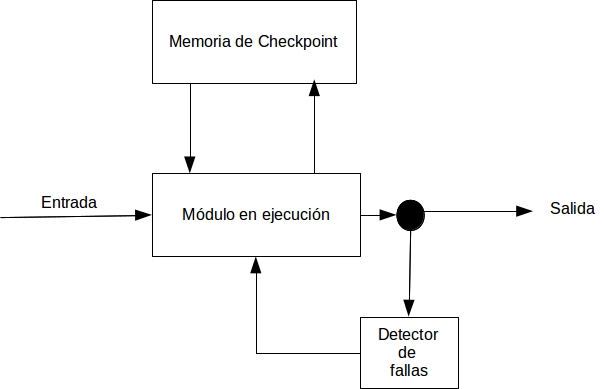
\includegraphics[scale=0.5]{images/Marco_teorico/checkAndRestart.jpg}
 \caption{Representación de checkpoint y restart}
 \label{fig:checkAndRestart}
\end{figure} 


Existe dos tipos de checkpoints, estáticos y dinámicos. Los checkpoints estáticos toman una 
``fotografía'' del estado del sistema antes de comenzar la ejecución del \ac{SW} y lo guarda en la
memoria \citep{FTDesign}. Si se detecta una falla, el sistema regresa a ese estado y 
comienza de nuevo su ejecución \citep{FTDesign}. Los checkpoints estáticos se basan en regresar el 
módulo a un estado predeterminado \citep{SoftwareFaultToleranceATutorial}. Se puede regresar a un 
estado inicial o a un set de estados predeterminados \citep{SoftwareFaultToleranceATutorial}.

Por otro lado se encuentran los checkpoints dinámicos. Estos usan checkpoints creados 
dinámicamente. Estas son imágenes del estado del sistema en varios puntos durante la ejecución 
\citep{SoftwareFaultToleranceATutorial}.

Hay tres formas de crear los checkpoints dinámicamente:
\begin{enumerate}
 \item Equidistantes, en el cual los intervalos que se crean los checkpoints son siempre iguales, 
los intervalos se elijen teniendo en cuenta el rate de falla \citep{FTDesign}. 
 \item Modular, en el cual los checkpoints se crean al principio o al final de la ejecución de un 
módulo. 
 \item Random, los checkpoints se crean aleatoriamente en el tiempo. 
\end{enumerate}

\subsubsection{Procesos pares}
Los procesos a pares utilizan dos versiones idénticas de un proceso de \ac{SW} que corre en 
procesadores separados (\citep{FTDesign}; \citep{SoftwareFaultToleranceATutorial}). El mecanismo de 
recuperación que se utiliza es el de checkpoint y restart \citep{SoftwareFaultToleranceATutorial}.  

Como se puede observar en la figura~\ref{fig:repPares}\footnote{Basada en \cite{FTDesign} y 
\cite{SoftwareFaultToleranceATutorial}} el primer procesador se encuentra activo. Este envía un 
checkpoint al segundo procesador. Si una falla se detecta, el primer procesador se apaga y se cambia 
al segundo procesador. El segundo procesador carga el checkpoint y continua con la operación.Toma el 
rol del primer procesador \citep{SoftwareFaultToleranceATutorial}. Luego el 
primer procesador realiza un auto test para verificar si el problema continua. Si se encuentra que 
este procesador sigue teniendo problema, se continúa trabajando con el segundo procesador 
\citep{FTDesign}.

La principal ventaja que brinda este mecanismo según \cite{FTDesign} es que permite entregar el 
servicio ininterrumpidamente.

\begin{figure}[h]
 \centering
 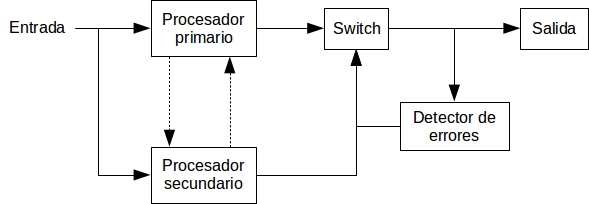
\includegraphics[scale=0.6]{images/Marco_teorico/repPares.jpg}
 \caption{Representación del proceso pares}
 \label{fig:repPares}
\end{figure} 

\begin{comment}

\begin{figure}[h]
 \centering
 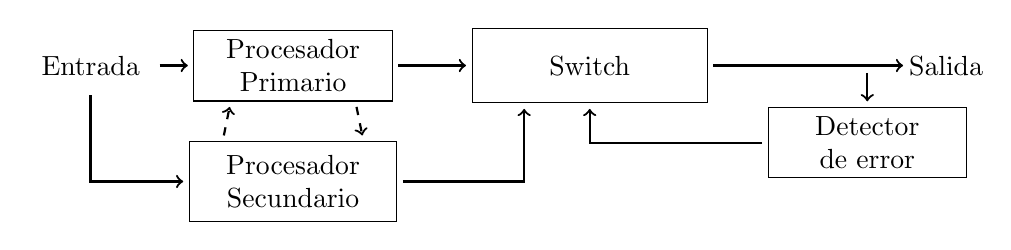
\begin{tikzpicture}[node distance=1cm, auto,]
  % definicion de estilos
  %Define style for boxes
   \tikzset{
   cuadro/.style={
           rectangle,
           draw=black,
           text width=6.5em,
           minimum height=2em,
           text centered},
    % Define arrow style
    arrow/.style={
           ->,
           thick,
           shorten <=2pt,
           shorten >=2pt,}	
    }
  \tikzstyle{circulo} = [draw, fill=black, circle, node distance=1cm, minimum size=5pt, inner 
sep=3pt]
    
  % Gráfico
  \node[inner sep=5pt] (entrada) {Entrada};
  \node[cuadro, right=0.5cm of entrada] (prim) {Procesador Primario};
  \node[cuadro, inner sep=5pt,below=0.5cm of prim] (secu) {Procesador Secundario};
  \node[cuadro, inner sep=10pt, right=1cm of prim] (selec) {Switch};
  \node[inner sep=0pt, right=2cm of selec](ghost1){};
  \node[cuadro, below=0.5cm of ghost1](detector) {Detector de error};
  \node[inner sep=0pt, right=0.5cm of ghost1] (salida) {Salida};
  
  \draw[arrow] (entrada)--(prim);
  \draw[arrow] (entrada)|-(secu);
  \draw[arrow, dashed] (prim.-30) -- (secu.30);
  \draw[arrow, dashed] (secu.150) -- (prim.-150);
  \draw[arrow] (prim)--(selec);
  \draw[arrow] (secu)-|(selec.-150);
  \draw[arrow] (detector)-|(selec);
  \draw[arrow] (selec)--(salida);
  \draw[arrow] (ghost1)--(detector);
 \end{tikzpicture}
 \caption{Representación del proceso pares}
 \label{fig:repPares}
\end{figure}

\end{comment}

\subsubsection{Diversidad de datos}
La diversidad es una técnica utilizada para mejorar la eficiencia en los checkpoint y restart, 
usando diferentes entradas por cada reinicio. Esto se basa en que las fallas en el 
\ac{SW} son dependientes de las entradas. Es poco probable que la misma falla se 
de con la misma secuencia de entrada \citep{FTDesign}.

\subsubsection{Bloques de recuperación}

Esta técnica combina las bases de la técnica de checkpoints y restart enfocada con múltiples 
versiones de un componente de \ac{SW} en el sentido de que una versión de \ac{SW} diferente es 
lanzada cada vez que se encuentra una falla. Los 
checkpoints son creados antes de que una versión de \ac{SW} se ejecuta.
La ejecución de las múltiples versiones pueden ser 
secuencial o paralelas dependiendo de la disponibilidad de la capacidad de procesamiento y 
perfomance requerida \citep{SoftwareFaultToleranceATutorial}.

%La representación de esta técnica se puede observar en el figura~[AGREGAR IMAGEN].
Las 
versiones son diferentes implementaciones de un mismo programa. Solo una de estas versiones provee 
la salida del sistema. Si un error es detectado por el test de aceptación, se vuelve hacia atrás, 
se retoma el último checkpoint, y se vuelve a ejecutar el módulo de \ac{SW} pero con una 
versión diferente a la que se ejecutó anteriormente \citep{FTDesign}.  	

Los checks del test de aceptación deben mantenerse simples para mantener la velocidad de la 
ejecución \citep{FTDesign}.

\begin{comment}
\begin{figure}[h]
 \centering
 \begin{tikzpicture}[node distance=1cm, auto,]
  % definicion de estilos
  %Define style for boxes
   \tikzset{
   cuadro/.style={
           rectangle,
           draw=black,
           text width=6.5em,
           minimum height=2em,
           text centered},
    % Define arrow style
    arrow/.style={
           ->,
           thick,
           shorten <=2pt,
           shorten >=2pt,}	
    }
       
  \tikzstyle{circulo} = [draw, fill=black, circle, node distance=1cm, minimum size=5pt, inner 
sep=3pt]
    
  % Gráfico
  \node[inner, sep=5pt] (input1){Entrada 1};
  \node[inner, sep=5pt, below=0.5cm of input1] (input2){Entrada 2};
  \node[inner, sep=5pt, below=0.5cm of input2] (puntos1){...};
  \node[inner, sep=5pt, below=0.5cm of puntos1] (inputn){Entrada n};
  \node[cuadro, right=0.5cm of input1] (version1){Versión 1};
  \node[cuadro, right=0.5cm of input2] (version2){Versión 2};
  \node[inner, sep=5pt, right=2cm of puntos1](puntos2){...};
  \node[cuadro, right=0.5cm of inputn] (versionn){Version n};
  
  \node[cuadro, above=1cm of version1] (check) {Memoria Checkpoint};
  \node[cuadro, right=1cm of version2] (switch) {Swith n a 1};
  \node[inner, sep=0pt, right=1cm of switch](ghost1){};
  \node[cuadro, below=0.5cm of ghost1](test){Test de aceptación};
  
  \node[inner, sep=0pt, right=0.5cm of ghost1](output){Salida};
 
  %Arrows
  \draw[arrow] (input1)--(version1);
  \draw[arrow] (input2)--(version2);
  \draw[arrow] (inputn)--(versionn);
  \draw[arrow] (version1)-|(switch.west);
  \draw[arrow] (version2)--(switch);
  \draw[arrow] (versionn)-|(switch.west);
  \draw[arrow] (ghost1)--(test);
  \draw[arrow] (switch)--(output);
  
  \draw[arrow, dashed] (check.-40) -- (version1.30);
  \draw[arrow, dashed] (version1.150) -- (check.-145);
  
  

 \end{tikzpicture}
 \caption{Configuración de bloques de recuperación}
 \label{fig:repPares}
\end{figure}
\end{comment}

%\subsubsection{Programación N-version}

%\subsubsection{Programación N-Auto Checking}



%Section that talk about dependability evaluation techniques
\section{Técnica de evaluación de fiabilidad}
La evaluación de la fiabilidad es de suma importancia para el desarrollo de sistemas críticos, ya
que permite identificar que aspectos del comportamiento del sistema juega un papel importante
\citep{FTDesign}.

\begin{enumerate}
 \item Modelado de un sistema en la fase de diseño.
 \item Aseguramiento del sistema en la fases finales de desarrollo (testing).
\end{enumerate}
El análisis confiabilidad tiene tres enfoques importantes:
\begin{itemize}
  \item Confiabilidad de \ac{HW}
  \item Confiabilidad de \ac{SW}
  \item Confiabilidad humana
\end{itemize}
En este trabajo de tesis se pondrá énfasis en el estudio en la confiabilidad del \ac{SW} a nivel de sistema.

La evaluación de la fiabilidad tiene dos aspectos. En primer lugar se tiene una \textit{evaluación
cualitativa} que permite identificar, clasificar y medir modos de fallas, o eventos combinacionales
que puedan provocar una falla. El otro aspecto es la \textit{evaluación cuantitativa}, la cual
permite evaluar en términos de probabilidad los atributos de la fiabilidad (Sección \ref{sec:atributos_de_la_fiabilidad}), disponibilidad, seguridad.

El análisis de confiabilidad es de gran importancia ya que provee información que es la base de la toma de desición. Esto es aplicado a diferentes áreas, tales como análisis de riesgos, protección ambiental, calidad, optimización de mantenimientos y operaciones y diseño de ingeniería \citep{Rausand04}.

\section{Medidas comunes de fiabilidad}
Las medidas de fiabilidad más comunes son las siguientes: failure rate, tiempo medio a la falla,
tiempo medio de reparación y tiempo medio entre fallas.

\subsection{Failure rate}
Failure rate $\lambda$ es el número esperardo de fallas por unidad de tiemp \citep{FTDesign}. Es
usual utilizar la dimensión \textit{fallas/horas}.

Generalmente, $\lambda$ se encuentra a nivel de componente. Para conocer el failure rate del
sistema completo, se puede realizar (a groso modo) una sumatoria de los $\lambda$ de los
componentes que integran el sistema. $$\lambda=\sum_{i=1}^{n} \lambda_i$$.

La evolución de $\lambda$ a través del tiempo, no tiene el mismo comportamiento tanto para \ac{HW} como para \ac{SW}
Si se devide el ciclo de vida de un sistema en las siguientes fases: mortalidad prematura (I), vida útil (II), desgaste (II) \citep{FTDesign}
se aprecia, para el caso del \ac{HW}, lo que se denomina \textit{curva de la bañera} la cual puede observarse en la Figura \ref{fig:bathtub_curve}.
En una primera fase, $\lambda$ decrese, ya que a través de los procesos de testing se van descubriendo y resolviendo los errores. Luego se da un periodo de estabilización.
Y al final, el \ac{HW} sufre el paso del tiempo, y se desgasta, aumentando la tasa de fallas.

\begin{figure}[h]
 \centering
 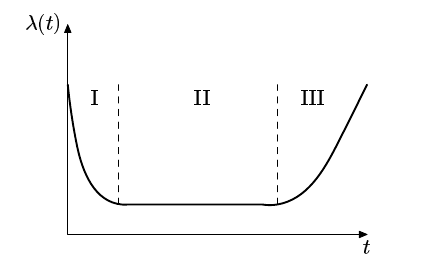
\includegraphics[scale=0.5]{images/Marco_teorico/bathtub_curve.png}
  \caption{Failure rate de HW vs tiempo }
\label{fig:bathtub_curve}
\end{figure}

Para el \ac{SW} es totalmente diferente. En primer lugar cuando se realiza una actualización, se aumenta la complejidad, como así también la probabilidad de fallas,
con ello el failure rate. Otra diferencia sustancia con el \ac{HW} es que el \ac{SW} no se desgasta con el tiempo. En la Figura \ref{fig:Failure_rate_software}
se aprecia $\lamda$ a través de tiempo. Esta curva suele llamarse \texit{curva serrucho}. El failure rate del \ac{SW} decrece en función del tiempo. En estos tipo de sistemas
la tasa de falla depende de varios factores como pueden ser el proceso utilizado en el diseño y codificación, complejidad del \ac{SW}, tamaño del \ac{SW},etc \citep{FTDesign}.

\begin{figure}[h]
 \centering
 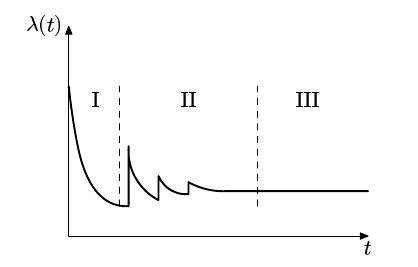
\includegraphics[scale=0.5]{images/Marco_teorico/Failure_rate_software.png}
  \caption{Failure rate SW vs tiempo }
\label{fig:Failure_rate_software}
\end{figure}

A lo largo de la vida de sistema se supone el failure rate $\lambda$ como constante. Por lo tanto la confiabilidad del sistema varía exponencialmente
con respecto al tiempo \citep{FTDesign}: $$R(t) = e^{- \lambda t}$$

Esto se conoce como \textit{ley de la falla exponencial}\citep{FTDesign}. El gráfico de confiabilidad $R(t)$ vs tiempo se muestra en la Figura \ref{fig:failure_rate}.

\begin{figure}[h]
 \centering
 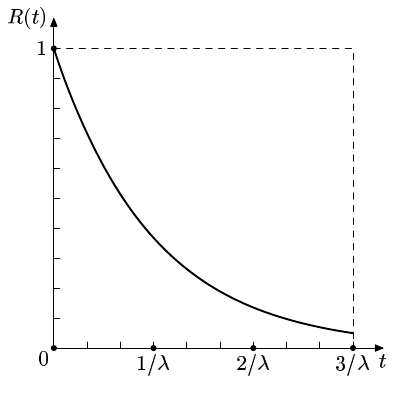
\includegraphics[scale=0.5]{images/Marco_teorico/failure_rate.png.png}
  \caption{Confiabilidad vs tiempo }
\label{fig:failure_rate}
\end{figure}

\subsection{Tiempo medio medio de falla}
\textit{El tiempo medio de falla} (MTTF\footnote{Del inglés, Mean Time To Failure}) de un sistema es el tiempo esperado que transcurra hasta la primera falla que se
detecte en el sistema. En terminos de confiabilidad, MTTF se define de la siguiente manera \citep{FTDesign} \citep{Rausand04} $$\int_0^{\infty} R(t) dt$$

\subsection{Tiempo medio de reparación}
\textit{El tiempo medio de reparación}(MTTR\footnote{Del inglés, Mean Time To Repair})de un sistema, es el promedio de tiempo que se requiere para reparar al sistema.
MTTR se especifica en términos de la tasa de reparación $\mu$ \citep{FTDesign} \citep{Rausand04}, el cual es el número esperarado de reparaciones por unidad de tiempo: $$MTTR = \frac{1}{\mu}$$

El MTTR depende de los mecanismos de recuperación ante fallas que se utilicen en el sistema, localización del sistema, scheduler de mantenimiento \citep{FTDesign}. Con esto se puede definir la disponibilidad como sigue: $$A(\infty) = \frac{MTTF}{MTTF+MTTR}$$

Muchas veces se utiliza MDT (\footnote{Del inglés, Meann Downtime}) en vez de MTTR, para denotar más claro que es el tiempo medio que el sistema se encuentra fuera de sericio.

\subsection{Tiempo medio entre fallas}
\textit{El tiempo medio entre fallas}(MTBF\footnote{Del inglés, Mean Time Between Failure}) de un sistema es el tiempo promedio entre dos fallas del sistema. $$MTBF = MTTF + MTTR$$

\subsection{Cobertura de fallas}
La cobertura de fallas es la probabilidad  de que el sistema no interrumpirá su actividad cuando una falla se presente. En términos matemáticos la cobertura
de fallas la probabilidad condicional $P(A|B)$. Existen diferentes coberturas de fallas, dependiendo de si se está tratando con detección de fallas, localización de fallas, contención de
fallas o recuperación de fallas \citep{FTDesign}. Siendo $A$ detección, localización, contensión o recuperación de fallas, y $B$ la existencia de fallas.

\section{Métodos de cálculos de fiabilidad}
Para evaluar la fiabilidad de sistemas se pueden utilizar diagramas de bloque de confiabilidad y procesos de Markov \citep{FTDesign}

\subsection{Diagramas de bloques de confiabilidad}

\subsubsection{Cálculo de confiabilidad}
Para medir la confiabilidad de un sistema mediante diagrama de bloques, se debe dividir el sistema objetivo en  partes paralelas y en serie. Se computa la confiabilidad
de las partes. La confiabilidad del sistema estará compuesta por la confiabilidad de ambas partes \citep{FTDesign}. Entonces
$$R(t) = \left \{
\begin{matrix}
  \prod_{i=1}^{n} R_{i}(t) & \text{para estructuras en serie}\\
  1 - \prod_{i=1}^{n}(1-R_{i}(t)) & \text{para estructuras en paralelo}
\end{matrix} $$
Esto nos indica que un sistema paralelo, es más confiable que uno en serie, aún así si sus componentes son menos confiables. Tal como ejemplifica \cite{FTDesign}, si se diseña un sistema en serie de 100 componentes, con una confiabilidad de 0.999, el sistema completo tendrá una confiabilidad de:
$0.999^100 = 0.905$. Mientras que, para un sistema paralelo, con solo cuatro componentes, con una confiabilidad menor (0.95) la confiabilidad del sistema
será $1-(0.95)^4 = 0.99999375$. El punto en contra de los sistemas paralelos, es que representan un costo mayor que las estrucutras en serie \citep{FTDesign}.

\subsubsection{Cálculo de disponibilidad}
Si se asume que el tiempo de falla y de recuperación son independientes, entonces se puede utilizar diagramas de bloques para calcular la disponibilidad
del sistema  \citep{FTDesign}.  Se puede observar que el cálculo es similiar al calculo de confiabilidad.
 $$A(t) = \left \{
 \begin{matrix}
   \prod_{i=1}^{n} A_{i}(t) & \text{para estructuras en serie}\\
   1 - \prod_{i=1}^{n}(1-A_{i}(t)) & \text{para estructuras en paralelo}
 \end{matrix} $$

\subsection{Utilización de procesos de Markov}
El principal objetivo del análisis de los procesos de Markov es calcular $P_i(t)$ la probabilidad de que el sistema se encuentre en el estado $i$
en el tiempo $t$. Con esto se puede calcular facilmente la confiabilidad, disponibilidad o seguridad del sistema \citep{FTDesign}.

Para determinar $P_i(t)$ se debe derivar una serie de ecuaciones diferenciales, una por cada estado del sistema. Estas ecuaciones se denominan ecuaciones de estado de transición. Las ecuaciones de los estados de transición se representan en una matriz $M$ denominada \textit{matriz de transición}. Cada elemento $m_{ij}$ de la matriz $M$ es un rate de transición entre los estados $i$ y $j$
$$M = \left [
\begin{matrix}
  m_{11}  & m_{12}  & ... & m_{k1} \\
  m_{12}  & m_{22}  & ... & m_{k2} \\
          &         & ... &        \\
  m_{1k}  & m_{2k}  & ... & m_{kk} \\
\end{matrix}
\right ]
$$

Haciendo $P(t)$ un vector en el cual el $i-ésimo$ elemento es la probabilidad $P_i(t)$ de que el sistema se encuentra en el estado $i$ en el tiempo $t$. Con ello se tiene: $$\frac{d}{dt}P(t) = MP(t)$$ \citep{FTDesign}.

Para calcular confiabilidad, disponibilidad y seguridad solo es necesario reemplazar en la matriz $M$ los rate correspondientes.

\chapter{Estado del arte}\label{chap:estado_del_arte}
% section that explain binary tree
%TODO: Arboles binarios
\begin{comment}
 Bibliografía utilizada aquí:
 
 \cite{Raghavendra84} -> Fault tolerance in Binary Tree Architecture
 
\end{comment}


\section{Árboles binarios}\label{sec:binary_tree}
El concepto de arquitecturas de árboles binarios es aplicable en el desarrollo de sistemas de 
computadoras jerárquicas, y sobre todo en computadoras de alta perfomance \citep{Raghavendra84}. 
Existen dos diferentes mecanismos de tolerancia a fallas \citep{Raghavendra84}:
\begin{enumerate}
 \item Esquemas con back up.
 \item Esquemas con degradación de perfomance.
\end{enumerate}

Teniendo en cuenta que estas arquitecturas son aplicadas principalmente en la construcción de 
circuitos VLSI\footnote{Del inglés, Very Large Scale Integration} \citep{Singh91}, se asume su 
aplicabilidad a arquitecturas de aviónica. 

La \ac{FT} y la perfomance de los sistemas dependen de las capacidades de las redes que se utilizan 
para la comunicación entre unidades de procesamiento \citep{Raghavendra84}. 

Un árbol binario está compuesto por nodos y enlaces (links). Existe un nodo central dónde se 
desprenden dos nodos hijos, estos se encuentran enlazados al nodo padre. Así recursivamente, se 
van generando dos nuevos hijos, por cada uno de los nodos. Los árboles binarios están divididos en 
niveles, que representa cada una de las generaciones de nodos.

Este tipo de topología tiene algunos problemas que la \ac{FT} debe hacer frente. En las 
arquitecturas basadas en árboles binario, existe una cierta probabilidad de que un nodo o un link 
falle \citep{Raghavendra84}. Las arquitecturas de árbol binario son en general físicamente 
estáticas. Por lo tanto, cualquier falla en uno de sus nodos (o links) demandaría una avería a 
nivel sistema, lo cual daría lugar a una pérdida de misión. Para ello se debe dotar a la 
arquitectura de un mecanismo de reconfiguración.

La tolerancia a fallas en arquitecturas binarias ya fueron estudiadas en profundidad en 
\cite{Hayes76}, \cite{Raghavendra84}, \cite{Singh91}. Para lograr \ac{FT} en estas arquitecturas se 
las deben diseñar con un número mínimo de nodos de backup y links redundantes, de modo tal de hacer 
frente cualquier punto de falla simple en la arquitectura. 

\subsection{Esquema de árbol binario con backups}
El esquema planteado por \cite{Raghavendra84} es similar al que se muestra en al Figura 
\ref{fig:binary_tree}. En este esquema se agregan nodos y links redundantes como técnica de \ac{FT}. 
Existe un nodo de backup por cada nivel del árbol.

\begin{figure}[h]
 \centering
 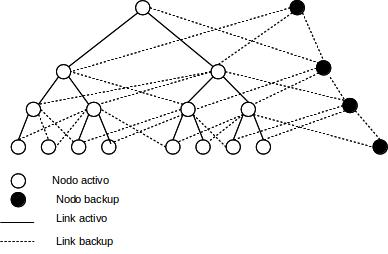
\includegraphics[scale=1]{images/Marco_teorico/binary_tree}
  \caption{Árbol binario de 4 niveles}  
\label{fig:binary_tree} 
\end{figure}

Esta arquitectura cuenta con una restricción, la cual indica que solo se puede tolerar una 
falla singular, por cada nivel de la arquitectura. Arquitecturas de este tipo, podrían tolerar más 
de una falla, sólo si se dan en diferentes niveles del árbol \citep{Raghavendra84}. Para agregar 
más tolerancia, se deberían agregar más redundancias.

Notese en la Figura \ref{fig:binary_tree} que cuando una unidad de procesamiento (nodo) falla, 
todos los links se deben reajustar hacia el nodo de la derecha. En este punto es importante 
mencionar, que ante esta situación se requiere una reconfguración a nivel de \ac{HW}, además de una 
reconfiguración a nivel de \ac{SW}. Es necesario algoritmos de ruteo dinámicos, de modo tal de 
conocer los nuevos caminos que intercomunican nodos, para mantener la operabilidad del sistema.  

\subsubsection{Estimación de la confiabilidad de un árbol binario con backup}\label{subsec:conf_binary_tree}
Se asume que la probabilidad de fallas de los links es muy baja en comparación con la de los nodos. 
Teniendo que el rate de falla es de $\lambda$, la confiabilidad  de un nodo es $R = e^{-\lambda 
t}$. También se sabe que un árbol binario con n niveles,  tiene $2^n - 1$ nodos en total. 
Entonces la confiabilidad de todo el sistema es: $$R_{nr} = R^{2^n - 1}$$

\cite{Raghavendra84} incluye en sus cálculos un factor de cobertura $c$, el cual es la probabilidad 
condicional de que se lleve a cabo una recuperación exitosa, luego de que una falla se haya 
detectado. Entonces la confiabilidad del sistema para una arquitectura de árbol binario con 
redundancias (un nodo backup por nivel) es el siguiente: $$R_{sys} = \prod_{k=0}^{n-1}{[R^{2k +1} + 
R^{2k}(1-R) + 2^kcR^{2k}(1-R)]}$$.

Simplificando: $$R_{sys} = R^{2n +1} \prod_{k=0}^{n-1}{[(2^kc+1) - 2^kcR]}$$

En la Figura \ref{fig:Reliability_binary_tree_4_levels}, se observa la confiabilidad de una 
arquitectura de árbol binario de 4 niveles, con una cantidad de $2^4 -1 = 15$ nodos. En color negro 
se grafica una arquitectura sin redundancia, mientras que en color rojo, azul y cyan, se muestra 
arquitecturas redundadas con diferentes $c$ (0.98, 0.99, 1, respectivamente). 

\begin{figure}[h]
 \centering
 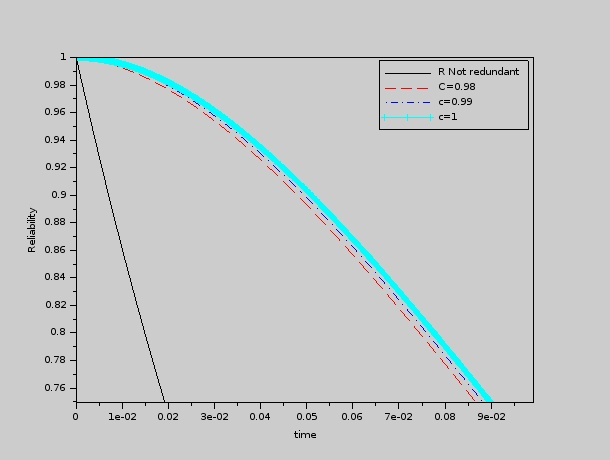
\includegraphics[scale=0.5]{images/Marco_teorico/Reliability_binary_tree_4_levels.jpg}
  \caption{Confiabilidad con respecto al tiempo de una arquitectura de árbol binario de 4 niveles}  
\label{fig:Reliability_binary_tree_4_levels} 
\end{figure}

Con esto podemos indicar, como es de esperarase, una arquitectura de árbol binario redundanda 
permite mantener un alto nivel deseable de confiabilidad, durante un mayor lapso de tiempo, a 
diferencia de un sistema no redundando. También se puede concluir que con un factor de cobertura $c$
más próximo a uno, maximiza los niveles de confiabilidad con respecto al tiempo. 

%\subsubsection{Extensión de la arquitectura con backup}

%\subsection{Esquema de árbol binario con degradación de perfomance}

% section that explain the hypercube systems
\section{Sistemas Hypercube}
Hypercube es una técnica utilizada para
conectar múltiples procesadores. Esta topología
tiene propiedades de tolerancia a fallas de un
componente, ya que si esto se produce, no se
transmite a todo el sistema \citep{Rong96}. Otra ventaja que
presenta esta topología es la disponibilidad de
enlaces entre cualquier par de nodos \citep{Mostafa14}. Un
hypercube n-dimensional tiene: $$2^n $$ nodos y $$n2^{n-1}$$ enlaces.
Los nodos está conectados a n nodos vecinos a través de n enlaces \citep{Rong96}. Estas
relaciones pueden ser representadas en forma de matrices de proximidad \citep{Mostafa14}.
En \cite{Mostafa14} se muestra una manera sencilla de calcular la confiabilidad
de sistemas de este tipo. La probabilidad de falla de la red ($p_n$) depende
de la probabilidad de falla de cada uno de los nodos ($p_n$), suponiendo
que todos los nodos tienen la misma probabilidad de falla la confiabilidad
del sistema sería: $$R(N) = 1 -(NP_v)$$.

Para calcular la confiabilidad de una red hypercube se debe seguir
la fórmula $$R(N) = 1 -(NP_v)$$, a esta se le realiza leves modificaciones
para obtener el siguiente cálculo de confiabilidad: $$ R_{sys} = 1 - [N(1-e^{- \lambda t})]$$

% section that explain Distributed network
\section{Redes distribuídas}
Una red de computadoras hace referencia a un conjunto de computadoras autónomas que se encuentran interconectadas, esto quiere decir que pueden intercambiar información \citep{Tanenbaum12}. Una red distribuída tiene como principal caraceterística que no existe un nodo central que "gestione" toda la red. Todas las cargas de las tareas y/o actividades son distribuídas entre los nodos que forman parte de la red.

Una red distribuída es tolerante a fallas si los nodos pueden formar subredes \citep{Stivaros92}. Es decir, la red se debe mantener activa y conectada, con diferentes topologías e interconexiones, que permitan tolerar posibles fallas producidas en algunos nodos y permitir mantener la perfomance \citep{Stivaros92}. Debido a que el procesamiento de la red se encuentra distribuída en todo el sistema, esto brinda una ventaja por encima a los sistemas centralizados desde el punto de vista de la confiabilidad \citep{Pradhan82}. Un componente importante de las redes distribuídas tolerantes a fallas, es la topología del sistema \citep{Pradhan82}.

Siguiendo la notación de \cite{Pradhan82} para describir la topología del sistema se utiliza, un gráfico sin direccionamiento G = <V,E>, donde V representa un set de nodos y E representa un set de relaciones. \cite{Stivaros92} agrega que $V(G) = \{v_1,v_2,v_3, ... v_n \}$ representa un vector de nodos, los cuales tiene probabilidades de operación $P = (p_1, p_2, p_3, p_n)$; y define una función de asignación $\pi$, la cual es una función que asigna V con una probabilidad $P_{\pi(v)}$.

La \ac{FT} de la red G, dado el vector de probabilidades \vec{P} y una función de asignación $\pi$, tal como se viene discutiendo anteriormente, es la probabilidad de que la red continúe funcionando, es decir continúe conectada, aún en la falla (aleatoria) de alguno de sus nodos, esto se denota $FT(G;\vec{P},\pi)$.

Se dice que un subset de nodos S, es un estado tolerante del sistema G, cuando estos nodos se mantienen conectados y funcionales. Se utiliza $\theta$ para indicar el conjunto de todos los S posibles. Un estado tolerante S contribuye $\prod_{v\in S}{P_{\pi (v)}} \prod_{v \notin S} (1-p_{\pi (v)})$ a la probabilidad de \ac{FT}.

Para calcular el total de la \ac{FT} del sistema, incluyendo todo los S, se hace: $$FT(G;\vec{P};\pi) = \sum_{S \in \theta}{Pr(S)} = \sum_{S \in \theta}{\prod_{v\in S}{P_{\pi (v)}} \prod_{v \notin S} (1-p_{\pi (v)})}$$

Una relación entre nodos es representado  como ij, lo cual representa un enlace bidireccional entre nodos. El grado del nodo i representa el número de relaciones que inciden en ese nodo, el cual se escribe $d_i$. Así, $d_i$ está limitado por el número de puertos de entrada y salida disponibles por cada nodo \citep{Pradhan82}. $k_{ij}$ representa el número mínimo de \textit{hop} (hop representa la transmisión a través de un link de datos)\citep{Pradhan82}

\cite{Stivaros92} y \cite{Pradhan82} mencionan la existencia de varias topologías que pueden ser aplicadas en una red distribuída tolerante a fallas. Una topología estrella posee una baja distancia entre nodos, pero una pobre tolerancia a fallas \citep{Pradhan82} \citep{Stivaros92}. La topología anillo, permite un simple ruteo, pero existen grandes distancias internodo. Un sistema completamente interconectado, presenta buenas características tolerantes a fallas, pero tiene un alto costo \citep{Pradhan82}. \cite{Pradhan82} propone una topología para una arquitectura distribuída de comunicación. Esta es una topología robusta, y puede llegar a ser compleja a medida que aumentan los nodos.

\subsection{Algoritmo de ruteo}
Los algoritmos de ruteos son necesarios en el desarollo de una arquitectura tolerante a fallas y reconfigurable. Los algoritmos de ruteo se los pueden dividr en dos: \textit{algoritmos primarios} y \textit{algoritmo alternativo}. El primero es utilizado cuando no hay fallas de nodos. Se deben mantener los caminos para llegar, correctamente, al nodo destino. El segundo se utiliza en la presencia de alguna falla, este requiere que sea capaz de detectar la presencia de fallas, para luego reconfigurar el sistema. Estos algoritmos deben ser simples y requerir una mínima cantidad de \ac{HW} y \ac{SW}.

Agregado a lo mencionado en el párrafo anterior, deben existir algoritmos de diagnóstico distribuído de falas, basados en los algoritmos de ruteo \citep{Pradhan82}.

% section that explain Ethernet Network
\section{Redes Ethernet en aviónica}\label{sec:ethernet}
TTEthernet es una tecnología de red de computadoras comercializada por TTTech Computertechnik AG para el desarrollo de aplicaciones seguras. SAE International\footnote{http://www.sae.org} estandarizó esta red como SAE AS6802. TTEthernet se basa en el Ethernet clásico, en el cual se pone énfasis en las características principales que deben respetarse en sistemas críticos, tales como latencias de mensajes determinísticos, presición de tiempo real, tolerancia a fallas \citep{Loveless15}. Tiene la capacidad de transmitir datos 100 veces más rápido que la que lo hacen las tecnologías tradicionales tales como el MIL-STD-1553.

El Ethernet clásico presenta ventajas, tales como su alta velocidad de transmisión de datos, flexibilidad, y su disponibilidad y bajo costo (ya que se trata de un componente COTS) \citep{Loveless15}, hacen deseable su aplicación en el área espacial. Fue utilizado en diferentes proyectos aeroespaciales y en misiones importantes tales como el Space Shuttler y la Estación Espacial Internacional (ISS) \citep{Loveless15}. A pesar de esto, el Ethernet no cumple con el determinismo requerido por las aplicaciones de tiempo real de un vehículo espacial. Por tal motivo, se desarrolla el sistema TTEthernet, el cual introduce un reloj de sincronización descentralizado, permitiendo la transmisión de mensajes \ac{TT}. En este tipo de red, existe una herramienta de planning que asigna a cada dispositivo un intervalo de tiempo, en el cual puede utilizar para transmitir frames. Estos sistemas utilizan Links Virtuales (VL) para permitir el envío de mensajes time-trigged. Cada VL es asociado con un time-trigged frame através de un identificador de tráfico crítico (CTID), este reemplaza el control de acceso al medio (MAC) \citep{Loveless15}. Una red simple se muestra en la Figura \ref{fig:Arq_TTEthernet}.

\begin{figure}[h]
 \centering
 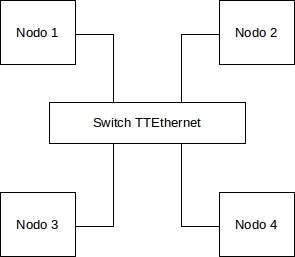
\includegraphics[scale=0.7]{images/Marco_teorico/TTEthernet_BUS.jpg}
  \caption{Arquitectura básica TTEthernet}
\label{fig:Arq_TTEthernet}
\end{figure}

TTEtheret puede actuar en dos clases de tráfico, con el objetivo de soportar diferentes niveles de cricticidad de mensajes. Estas clases de tráficos son las siguientes \citep{Loveless15} \citep{Steiner13}:
\begin{itemize}
	\item Time-Triggered, permite enviar mensajes de acuerdo a una planificación predefinida (scheduling),
	\item Rate-Constrained (RC), en el cual se llevan algunas restricciones de tamaño y rate de transmisión de frames,
	\item Best-Effort (BE), el cual se comporta de manera similar que el Ethernet
\end{itemize}

El paquete TTEthernet tiene una gran similitud con el frame del estándar IEEE 802.3 (Ethernet). Se denota en la Figura \ref{fig:Frame_TTEthernet} que en lugar de la MAC del 802.3 frame se divide en el CT Marker y el CTID. El primero es un identificador estático utilizado para distinguir paquetes \ac{TT} de otros tipos de tráficos.

\begin{figure}[h]
 \centering
 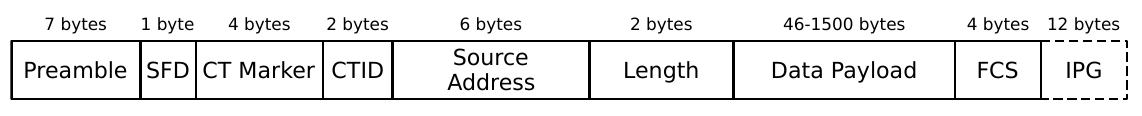
\includegraphics[scale=0.3]{images/Marco_teorico/Frame_TTEthernet.png}
  \caption{Frame de mensaje TTEthernet}
\label{fig:Frame_TTEthernet}
\end{figure}

El estándar SAE AS6802 define el protocolo de sincronización del TTEthernet. El protocolo TTP fue diseñado para reducir la complejidad de las arquitecturas distribuidas tolerantes a fallas \citep{TTTechWeb}. Existe un grupo de dispositivos de relojes locales que permite la sincronización requerida por la comunicación \ac{TT}, a esto se lo denomina \textif{dominio de sincronización} \citep{Loveless15}. Cada dominio de sincronización es asignado a uno de los siguientes roles:
\begin{itemize}
	\item Compression Master (CM)
	\item Synchronization Master (SM)
	\item Synchronization Cliente (SC)
\end{itemize}

\subsection{Experiencia de vuelo}
\cite{Loveless15} demuestra la aplicación de esta tecnología para computadoras de vuelo redundantes en misiones de naves simuladas. Esta tecnología toma tanto interés que el Sistema de Exploración Avanzada (AES)\footnote{Del ingles, Advanced Exploration Systems} de la \ac{NASA} lleva a cabo un proyecto denominado Avionics and Software (A&S). TTEthernet también fue utilizada en una arquitectura tolerante a fallas en el Integrated Power, Avionics and Software (IPAS)  del Johnson Space Center (JSC) y en el Core Flight Software (CFS) del Asteroid Redirect Mission (ARM) simulado\footnote{Los mencionados anteriormente son ejemplos de la utilización de TTEthernet} \citep{Loveless15}. También fue utilizado exitosamente durante la misión Orion \citep{TTTechOrion} .
TTEthernet simplifica el diseño de sistemas espaciales que deben contar con tolerancia a falla y una alta disponibilidad. La seguridad y la redundancia se mantiene sin ningún tipo de aplicación extra.

% section that explain the Bus network architecture
 \section{Arquitectura de red basada en BUS}
En \cite{Tai99} se presenta una arquitectura tolerante a fallas basada en BUS. Esta topología forma parte de un programa denominado X2000, el cual tiene como objetivo desarrollar una arquitectura tolerante a fallas y basada en componentes COTS. la cual pertenece a \ac{NASA}. Esta este programa se desarrolla bajo una filosofía de misiones espaciales la cual dice: "Más rápido, mejor, más económica" \footnote{En ingles, faster, better, cheaper}.

Esta arquitectura utiliza una topología novedosa denominada \textit{stack-tree topology} \citep{Chau99} \citep{Tai99}. Una stack-tree es un árbol donde cada nodo rama se encuentra conectado como mucho a tres otros nodos de los cuales, como máximo, dos son nodos ramas \citep{Tai99}. Una \ac{CST} es aquella en donde cada nodo rama está conectado al menos 1 nodo rama \citep{Tai99}.

En las Figura se pueden observar ejemplos de stack-tree. Mientra que en esta otra Figura no es una stack-tree.
\todo[inline]{Colocar las imagenes del paper BUS network architecture}

Como el objetivo principal es desarrollar una arquitectura tolerante a fallas, esto es, que aún cuando un nodo o un link entre nodos falle, el sistema completo debe continuar funcionando, sin ningún tipo de degradación en su servicio. Para cumplir con este objetivo \cite{Tai99} trabajan con un esquema de denominado \ac{CST} de equema dual (\ac{CST}$_D$) \footnote{En ingles,\ac{CST} dual scheme}. Esta puede observarse en la Figura
\todo[inline] {Colocar la imagen del paper, sonbre CSTd}

Para aumentar la confiabilidad de la arquitectra ante la acurrencia de fallas, se agrega links de backups que unen los nodos iniciales con el final, dando un efecto 3D de anillo \citep{Tai99}.

\subsection{Evaluación de la confiabilidad de arquitecturas basadas en BUS}
La confiabilidad de esta arquitectura (como ya se viene mencionando) es la probabilidad de que, a lo largo del tiempo de vida de la misión $t$, la arquitectura se encuentra funcional, en la cual todos los nodos (aquello que no hayn fallado) se encuentren conectados \citep{Tai99}. \citep{Tai99} y \citep{Chau99} asumen que la probabilidad de que un nodo falle es mucho mayor a que un enlace (el bus físico) falle.

En \cite{Tai99} indica que la confiabilidad de la red depende del tamaño $k$ (k es el número de nodos ramas). La confiabilidad de una red basada en \ac{CST} simplex es la probabilidad $U(k)$ de que los nodos no fallen, o que ante una falla se detecte y se lleve a cabo correctamente la reconfiguración del sistema. $$U(k) = (1-q) \sum_{j=0}^{k} {k}\choose{j} (1-q)^{k-j} (cq)^j $$ donde $q = 1-e^{-\lambda t}$ es la probabilidad de que un nodo falle durante el tiempo de vida de la misión $f$. Entonces $$R_s^{CST} = \sum_{k=1}^n (n-k+1)U(k)(cq)^{2(n-k)}$$ donde $(cq)^{2(n-k)}$ es la probabilidad que los  $2(n-k)$ nodos que conforman un cluster fallan, y esta falla es detectada y se lleva a cabo una correcta reconfiguración.

Para un \ac{CST} dual ocurre de manera similar. Se define $V(k)$ de la siguiente manera: $$V(k) = s(1-q)^k \sum_{j=1}^k {k}\choose{j} (1-q)^{k-j} (cq)^q + (1-q)^{2k}$$

Entonces la medida de $R_D^{CST} =  \sum_{k=1}^n (n-k+1) V(k) (cq)^{2(n-k)}$

% section that explain the modeling and metrics for critical system
\section{Métrica y modelado de la confiabilidad de sistemas}
Es de suma importancia llevar a cabo el análisis de la confiabilidad, disponibilidad y mantenibilidad (RAM\footnote{Del ingles, Realibility, Availability, Maintainability) de sistemas satelitales, durante la fase de diseño \citep{Hoque15}. Llevar a cabo esto, es de gran importancia, ya que permite el desarrollo de estrategias que permitan altos grados de confiabilidad, disponibilidad y mantenibilidad \citep{Hoque15}.

Existen dos categorías de medición de la confiabilidad y predición \citep{Schneidewind97}, estas son utilizadas para asegurar la seguridad del software de sistemas críticos \citep{Schneidewind97}, las cuales son:
  \begin{itemize}
    \item medición y predicción que están asociadas con las fallas y errores residuales.
    \item medición y predicción que están asociadas con la disponibilidad del sistema a sobrevir durante la misión sin experimentar fallas en el fallas (o pérdidas) en el sistema.
  \end{itemize}

  Las dos categorías mencionadas anteriormente son explicadas en \cite{Schneidewind97}.

  Según \cite{Liu14} las severidades de las fallas son clasificadas como críticas, peligrosas o triviales, teniendo en cuenta la contribución de esa falla a la pérdida de la misión. Es importante, además, conocer el riesgo de una falla. El riesgo, se define como la posibilidad de que una falla produzca una lesión (por ejemplo, un astronauta en vuelos tripulados), algún daño material (por ejemplo, la destrucción del satélite), o una pérdida (por ejemplo, la pérdida de la misión).

  Dependiendo de la misión, un criterio para definir si un sistema es seguro o no, es reduciendo las fallas que pueden provocar pérdidas de vida, pérdida de la misión o la obligación de abortar una misión \citep{Schneidewind97}. \cite{Schneidewind97} define dos criterios que deben satisfacerse:
  \begin{itemize}
    \item $r(t_t) < r_c$,
    \item $T_F(t_t) > t_m$
  \end{itemize}

  dónde $t_t$ es el Tiempo total de testing (observado o predicto); $r(t_t)$ son las fallas restantes hasta $t_t$; $r_c$ es una valor crítico de fallas restantes ;$T_F(t_t)$ es la métrica para medir el riesgo; y $t_m$ es la misión de la duración.

  Lo anterior signifca que un sistema crítico será seguro si: las fallas restantes en el tiempo de prueba son menores a un valor crítico de cantidad de fallas, o la duración de una misión es mayor al tiempo que se de la siguiente falla.
  
 En la literatura se utilizan modelos matemáticos para modelar los sistemas críticos y calcular así su confiabilidad. La mayoría de ellos asumen, que todas las fallas tienen igual tasa de detección de fallas, como así también la misma severidad, lo cual no es correcto \cite{Liu14}.


\chapter{Análisis y desarrollo de arquitectura tolerante a fallas}
\vspace{1cm}

\itshape
En este capítulo se lleva a cabo un estudio de la confiabilidad de tres tipos
de topologías tolerantes a fallas (Sección \ref{seccion:TopologiaEstudio}
página \pageref{seccion:TopologiaEstudio}), candidatas a ser utilizada en el
diseño de la arquitectura propuesta en este trabajo de tesis.

Para ello, en la Sección \ref{sec:req_analisis} (página \pageref{sec:req_analisis})
se realiza una descripción de algunos requerimientos (no estrictos), que guiarán
el desarrollo de una arquitectura para un misión satelital ficticia basada en
componentes COTS. En base a estos ``requerimientos'', se presentan los modelos para
la medición de confiabilidad de las topologías mencionadas en el párrafo anterior. 

En la Sección \ref{sec:protocolo_communicacion} (página \pageref{sec:protocolo_communicacion})
se describe resumídamente el protocolo CANae 0.1 Alpha, que está basado en CAN y
que fue desarrollado en este trabajo de tesis. En el apéndice \ref{Appendix:A}
se describe este protocolo con mayor detalle
\upshape

\noindent\rule{\textwidth}{2pt}

\vspace{1cm}
% section that make an introduction
%\chapter{Introducción}\label{chap:intro}
% TODO: Introuducción, extraída desde el plan de tesis,
En el marco del Plan Espacial Nacional, desarrollado por la \ac{CONAE} de Argentina, y con el propósito de llevar a cabo actividades de investigación y 
aplicación, provenientes de la \ac{UNLAM} se presenta este plan de tesis con el fin de ampliar los 
conocimientos y la participación de la \ac{CONAE} y \ac{UNLAM}, en el campo del Desarrollo Informático y 
Ciencias de la Computación.

Las actividades desarrolladas para este trabajo de tesis son realizadas, en su mayor proporción, en 
la Unidad de Desarrollo \ac{INVAP}, ubicada en San Carlos de Bariloche, Provincia de Río Negro. Este 
trabajo se encuentra orientado a brindar un nuevo conocimiento, que ayude en cierta medida, en el 
desarrollo de los diferentes proyectos con los que cuenta actualmente esta empresa, agregando un 
grado de innovación en el resultado que se obtenga.

\ac{INVAP} tiene como visión ser un referente en proyectos tecnológicos a nivel mundial \cite{invapWEB}, 
por lo tanto, debe asegurarse que cada uno de los productos que se lleven a cabo sean competitivos. 
Para lograr cumplir con esto, es necesario que tales proyectos se encuentren a la vanguardia 
tecnológica y científica.  

El desarrollo de proyectos satelitales conlleva costos de importante magnitud, y 
dependen de cada misión. Una parte importante de los costos está conformado por el 
desarrollo\footnote{\textit{Nota: entiéndase por desarrollo al proceso de planificación, análisis, 
diseño e implementación.}} y sobre todo los materiales que se utilizan para su fabricación. Esto 
es debido a que se utilizan componentes que son exclusivos para el ámbito espacial, en otras 
palabras que se encuentran ``calificados para volar''. Estos componentes son fabricados especialmente para soportar el ambiente hostil del espacio.

Si se considera al ámbito espacial como una industria, algo que ha sido demostrado en los últimos 
años; y si se tiene en cuenta las intenciones de crecimiento y competitividad de la empresa INVAP,  de permitir el ingreso de nuestro pais en el mercado satelital \cite{invapWEB}, resulta de gran 
importancia lograr reducir los costos en fabricación y desarrollo de vehículos satelitales.

La \ac{NASA} tiene un enfoque de desarrollo bajo el lema 
``faster, cheaper, better'' \cite{Forsberg99}, lo cual busca desarrollar sus proyectos y misiones 
de foma rápida, barata y mejor. Bajo este enfoque se han realizado diversos estudios e 
investigaciones dando resultados sumamente positivos \cite{Tai99}, \cite{Chau99}, 
\cite{Schneidewind98}, \cite{Forsberg99}. En estos trabajos se utilizan componentes que no se 
encuentran ``calificados para volar'',  los cuales también son llamados componentes \ac{COTS}, o de estantería. Debe mencionarse, que también hubo algunos 
fracasos en su aplicación. 

A simple vista, la utilización de estos componentes ayudaría a reducir costos. Sin embargo, esto 
no es tan directo. Los componentes \ac{COTS} al no estar calificados, se les deben realizar tareas 
de calificación adicional. Además deben ser aplicados a un ambiente, que asegure 
que no fallarán durante la misión; o si fallan, no será motivo de pérdida de la misma. 

Los componentes \ac{COTS} suelen tener un costo de compra entre 100 y 1000 veces menores que aquellos 
que está califcados para volar. Por lo que el aumento en la utilización de estos componentes, 
aplicados al desarrollo de diferentes tipos de satélite, \textbf{permitiría reducir los costos y 
ahorrar algunos millones de dólares del proyecto satelital.} Esto facilitaría el ingreso de 
Argentina en un mercado altamente competitivo.

El desafío de este trabajo de tesis es analizar y estudiar arquitecturas que sean tolerantes a 
fallas, que permitan una correcta comunicación entre los diferentes subsistemas de un vehículo 
espacial de nueva generación, y que tenga como característica principal un cierto grado de confiabilidad, de modo tal que pueda ser aplicado con componentes \ac{COTS}.

\section{Motivación}\label{chap:motivacion}
Los costos de un proyecto satelital se pueden clasificar, a grandes rasgos, en 5 grupos:
\begin{itemize}
 \item Desarrollo
 \item Materiales
 \item Ensamblado, integración, y tests
 \item Lanzamiento
 \item Operaciones
\end{itemize}

Este trabajo de tesis se centrará principalmente en el desarrollo (proceso de planificación, 
análisis, diseño e implementación.), y en los materiales utilizados en la fabricación de vehículos satelitales.

No se puede mencionar a ciencia cierta cuál es el costo “verdadero” de desarrollar un satélite. Este 
depende exclusivamente del tipo de satélite y de la misión. Lo que si se debe tener en claro es que 
las tareas de desarrollo representan una parte muy importante del costo total del proyecto.

Desarrollar un vehículo espacial con componente \ac{COTS}, en un principio podría representar costos 
adicionales, ya que se le deben realizar tareas de calificación adicional, debido a que no están 
“preparados” para resistir las condiciones hostiles del espacio. 

Uno de los puntos positivos, y que motivan la aplicación de componentes COTS, es que a la hora de 
desarrollar varios satélites en base a la misma ingeniería, se puede ahorrar en gran medida en los 
materiales que se utilizan. Los componentes \ac{COTS} suelen tener un costo de compra entre 100 y 1000 
veces menores que aquellos que están calificados para volar. \textbf{Esto ayudaría a ahorrar 
algunos millones de dólares de los proyectos satelitales.}
  
Otra de las ventajas de utilizar componentes \ac{COTS}, es que la mayoría cuentan con una tecnología más 
avanzada que aquellos que son calificados para volar. Esta tecnología permite:
\begin{itemize}
 \item Aumentar prestaciones, mediante el incremento de las capacidades de procesamiento, memoria, 
velocidades de 
procesamiento, etc.
 \item Implementar funciones que son imposibles de aplicar en tecnologías viejas.
 \item Reducir tiempos de desarrollo.
 \item Reducir volumen, masa y consumo
\end{itemize}

El último punto mencionado anteriormente es de especial interés, ya que al reducir volumen y masa, 
permite reducir costos adicionales como el de lanzamiento.

Esta reducción de costos de proyectos satelitales tienen ventajas directas a la hora de introducir a 
Argentina en un mercado altamente competitivo, donde la mínima reducción de estos, representa 
ganancias económicas importantes. 
 
Uno de los puntos en contra de la utilización de componentes \ac{COTS} es que al no ser calificados para 
volar, es necesario llevar a cabo tareas y estrategias inteligentes, con el fin de hacer frente a 
esa “deficiencia”. Por ello, se exige realizar una investigación y análisis de diferentes 
arquitecturas de aviónica, que puedan ser utilizadas para lograr que el sistema sea tolerante a 
fallas, y así, cumplir con los requerimientos de una misión satelital. 

El estudio de arquitecturas tolerantes a fallas, no solamente tiene aplicación en el ámbito 
espacial, si no que también puede ser extendido a cualquier sistema crítico, los cuales necesitan 
ser robustos y tolerantes a fallas, como es el caso de aviones comerciales, plantas nucleares, 
automóviles, etc.

% --------------------- %
% TODO: Hipótesis
% --------------------- %
\section{Hipótesis}
La hipótesis de esta tesis es la siguiente: ``Una arquitectura de aviónica  basadas en componentes 
\ac{COTS}, robusta y tolerante a fallas, es totalmente aplicable y utilizable en vehículos espaciales, 
con un alto nivel de confiabilidad, lo cual permite disminuir la complejidad de los sistemas actuales de aviónica''.

\section{Objetivo del trabajo y preguntas de investigación}

\subsection{Objetivo}
El objetivo de este trabajo es investigar y analizar arquitecturas de comunicación de los 
subsistemas de aviónica tolerante a fallas basada en componentes \ac{COTS} para vehículos 
satelitales de nueva generación.

% secondary objectives
\subsection{Objetivos Específicos}
\begin{enumerate}
 \item Realizar un estudio del estado de la cuestión sobre arquitecturas tolerantes a fallas para 
sistemas críticos.
 \item Investigar y analizar arquitecturas tolerantes a fallas que aseguren la confiabilidad del 
sistema y que sean aplicables en la industria satelital.
 \item Investigar y analizar protocolos de comunicación, para las capas superiores del modelo de 
OSI (modelo de interconexión de sistemas abiertos - ISO/IEC 7498-1), orientados a la tolerancia a 
fallas y confiabilidad de los sistemas. Realizar un estudio comparativo de los diferentes 
protocolos estudiados.
 \item Investigar una metodología para lograr una medición de la tolerancia a fallas en 
arquitecturas de aviónica.
 \item Desarrollar un estudio comparativo de arquitecturas tolerantes a fallas con el fin de obtener 
ventajas y desventajas de cada una de ellas.
 \item Diseñar modelos alternativos de arquitecturas tolerantes a fallas, que tenga un grado de 
confiabilidad tal que permita la aplicación de componentes \ac{COTS}.
 \item Evaluar la confiabilidad de los modelos de arquitecturas (mediante métrica desarrollada en 
este trabajo o siguiendo otras estrategias). 
 \item Proponer el diseño de una nueva arquitectura tolerante a fallas, con un 
grado de confiabilidad suficiente para la aplicación de componentes \ac{COTS} en aviónicas de vehículos 
satelitales.
\item Simular la arquitectura planteada para medir su grado de tolerancia a fallas y perfomance.
\end{enumerate}

% section that talk about requeriments
\section{Requerimientos para el análisis}
En esta sección no se pretende realizar una lista de requerimientos formales para el desarrollo de una arquitectura, esto se hace el capítulo siguiente. El objetivo de esta sección, es llevar a cabo una guía sencilla de las partes principales de un sistema satelital. Con esto en mente se podrá desarrollar diferentes topologías de comunicación, y luego analizar su tolerancia a falla.

Se supondrá una misión de 15 años (sin carga útil para simplificar el análisis) cuyo sistema estará compuesto por los siguientes subsistemas (en inglés para mantener correspondencia con la literatura) basado en \cite{Fontescue03}:
\begin{itemize}
\item Power Subsystem
\item Atitude and Orbit control Subsystem
\item Telemetry and Subsystem
\item Thermal Subsystem
\item Propulsion Subsystem
\item Data Handlig Subsystem
\end{itemize}

El sistema, entonces, está compuesto por 6 nodos. Los nodos se suponen computadoras con capacidad de procesamiento suficiente para cada subsistema. Cada una de estas computadoras/nodos es un componente COTS con un cierto grado de confiabilidad (se suponen lo suficientemente bajo como para no ser utilizado en forma directa en el desarrollo de satélites). A nivel de \ac{HW} estos nodos cuenta con tolerancia a fallas, lo que aumenta su confiabilidad. El subsistema de Data Handling tiene que tener comunicación con todos los subsistemas, ya que será la encargada de controlar el correcto funcionamiento del sistema, enviar comandos, y empaquetar telemetría de los sensores.




% section that talk about the nomenclautre
\section{Nomenclatura}
Durante el análisis se utilizará la siguiente nomenclatura:

\begin{tabular}{p{3cm}l l }

$T_m$       & Tiempo de la misión\\ \\
$TTNF$      & Tiempo hasta la siguiente falla\\ \\
$\lambda$   & Tasa de falla\\ \\
$MTBF$      & Tiempo medio entre fallas\\ \\
$MTTR$      & Tiempo medio de reparación\\ \\
$A(t)$      & Disponibilidad\\ \\
$R(t)$      & Confiabilidad\\ \\

\end{tabular}

Como se definió anteriormente el $T_m$ es de 15 años. Para simplificar los trabajos de cálculos y ejecución del presente trabajo, se supone que la arquitectura puede fallar solo una vez durante la misión satelital. Por lo tanto, el $TTNF$ será de 15 años. La tasa de falla se define como: $$\lambda = \frac{1}{15}$$ Suponiendo que la arquitectura no debería fallar durante los 15 años de misiones se da la siguiente sisituación: $$MTTBF = MTTR = 15 $$ Por otro lado, La disponibilidad es $A(t) = 99\%$. La confibialidad, como se estudió en secciones anteriores, es $R(t) = e^{- \lambda t}$



% section that talk about the differents topology
\section{Estudio de topologías de arquitecturas}
Luego de un estudio exhaustivo del estado de la cuestión (\autoref{chap:estado_del_arte}) se llegó a la conclusión de que las topologias más estudiadas, por ende más maduras y sencillas de aplicar a las activiades que se pretenden realizar en la presente tesis son:
\begin{itemize}
  \item Árbol binario
  \item Red distribuída
  \item Arquitectura hypercube
\end{itemize}

En esta sección, se definirá modelos para medir la confiabilidad de cada una de las topologías de arquitectura que aseguren una mayor tolerancia a fallas a nivel de sistema, de modo tal que si se llega a producir una falla en cualquiera de los nodos (sistemas de procesamiento) de la arquitectura, esta puede reconfigurarse, pemitiendo que esta continúe funcionando, sin sufrir ningún tipo de degradación, aún en la presencia de fallas. 

\subsection{Árbol binario}
En primer lugar se planteó un árbol binario de cuatro niveles con back up, basandose en el diseño de \cite{Raghavendra84} \ref{fig:Reliability_binary_tree_4_levels}. Este diseño cuenta con $2^n - 1 =  15$ nodos. De lo estudiado en \autoref{sec:binary_tree} la confiabilidad puede ser calculada de la siguiente manera: $$R_{sys} = R^{2n +1} \prod_{k=0}^{n-1}{[(2^kc+1) - 2^kcR]}$$

Con esto se puede observar la confiabilidad de la red con respecto al tiempo \ref{fig:Reliability_binary_tree_4_levels_2}.

\begin{figure}[H]
 \centering
 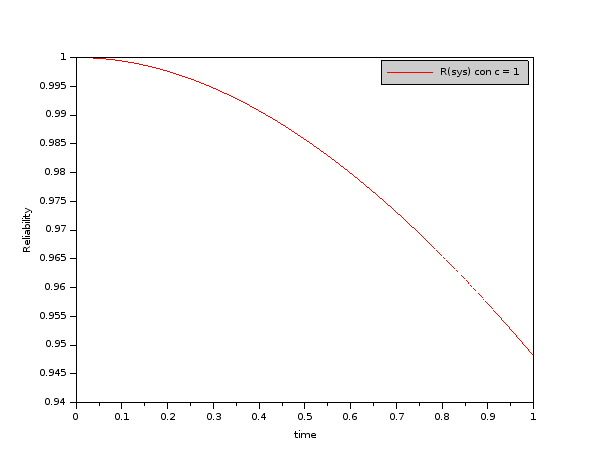
\includegraphics[scale=0.5]{images/Capitulo4/Reliability_BinaryTree.png}
  \caption{Confiabilidad con respecto al tiempo de árbol binario de 4 niveles}  
\label{fig:Reliability_binary_tree_4_levels_2} 
\end{figure}

La cantidad de niveles que se eligió para esta topología depende del número de subsistemas que se requieren.

Los nodos back up se mantienen inactivos, es decir no participan en el procesamiento durante la vida normal del sistema. En caso de producirse una falla, se supone que estos nodos de redundancia, comienzan a funcionar automáticamente, sin ninún tipo de retraso. Esto, que no corresponde con la realidad, permite simplificar los cálculos para este trabajo de tesis.

\subsection{Red distribuida}
El estudio de una topología de red distribuída no es tan sencilla como la que se plantea para un árbol binario. Para el desarrollo de esta red, además de los 6 nodos que representa cada uno de los subsistemas requeridos, se agrega 2 nodos de redundancia. Por lo tanto se tiene una red de 8 nodos. Siguiendo la metodología de desarrollo presentado por \cite{Pradhan82} se llevó a cabo la red que se presenta en la Figura \ref{fig:distributed_net}. 

\begin{figure}[h]
 \centering
 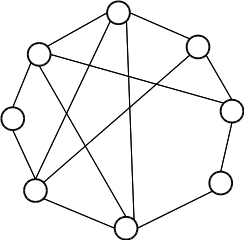
\includegraphics[scale=0.75]{images/Capitulo4/distributed_network.jpg}
  \caption{Red distribuida}  
\label{fig:distributed_net} 
\end{figure}

Esta cuenta con 4 nodos de grado 4, 2 nodos de grado 3, y 2 nodos de grado 2. Ante cualquier falla de alguno de los nodos de la red, esta topología tiene la capacidad formar subredes, que mantien todos los nodos conectados (a excepción del fallado), asegurandose la funcionalidad y reconfiguración del sistema completo. Estratégicamente y para lograr la condición mencionada anteriormente, se crea la \textbf{condición} de que pueden fallar hasta 4 nodos simultaneamento. Esto aseguraría de que la red continuará funcionando aún en la presencia de fallas (tolerante a fallas).

Se modificó la fórmula desarrollada  por \cite{Stivaros92}, para lograr una cohrencia de los modelos que se vienen planteand en el presente trabajo. Teniendo en cuenta que la confiabilidad del sistema completa es: $$R(t) = \prod_{v \in S} e^{- \lambda t}$$

donde $v$ representa el nodo y $S$ es el subsistema funcional. Es decir, que este modelo recorre todos los nodos funcionales. Cuando existen nodos con fallas, y que dejan de ser funcionales, el modelos es el siguiente: $$R_{sys} =\sum_{i=0}^{k} (( \prod_{v \in S} R(t)) - (\prod_{v \notin S} (1 -  R(t) c )))$$

donde c se definió como una \textit{constante de degradación del sistema} para modelar una degradació del sistema.

En la Figura \ref{fig:reliability_distributedNet} se puede observar la \textit{curva de confiabilidad} del sistema, para el caso en el que todos los nodos se encuentran funcionales. 

\begin{figure}[H]
 \centering
 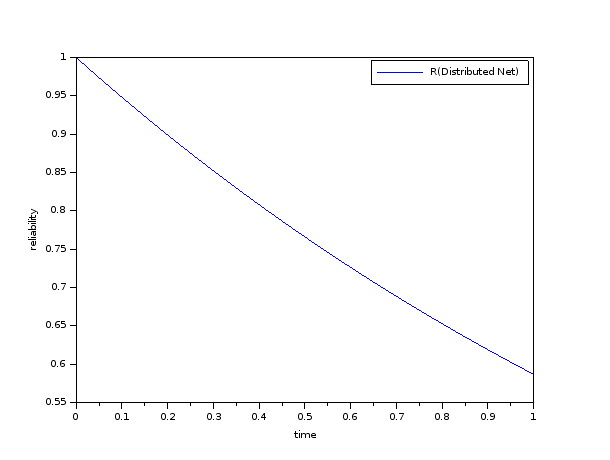
\includegraphics[scale=0.5]{images/Capitulo4/Reliability_DistributedNet.png}
  \caption{Red distribuida}  
\label{fig:reliability_distributedNet} 
\end{figure}


Para el caso de la falla de todos los nodos la \textit{curva de confiabilidad} (Figura \ref{fig:reliability_distributedNet_4Nodes_Fail}) muestra correctamente la degradación esperada de la confiabilidad, con respecto al sistema funcionando correctamente sin ninguna falla.

\begin{figure}[H]
 \centering
 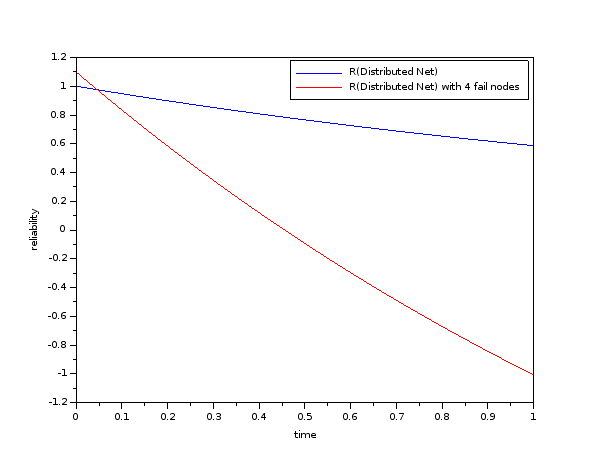
\includegraphics[scale=0.5]{images/Capitulo4/Reliability_DistributedNet_4Nodes_Fail_2.png}
  \caption{Red distribuida}  
\label{fig:reliability_distributedNet_4Nodes_Fail} 
\end{figure}

\subsection{Red hypercube}
Para el caso de la red hypercube se llevaron a cabo modificaciones al modelo planteado por \cite{Mostafa14}, con el propósito de mantener coherencia en los modelos y cálculos que se realizan en este trabajó. Se diseñó una red 3-dimensional, con 8 nodos,  de los cuales 6 nodos corresponden a los diferentes subsistemas y 2 nodos son utilizados de redundancia (Figura \ref{fig:Reliability_Hypercube}).

\begin{figure}[H]
 \centering
 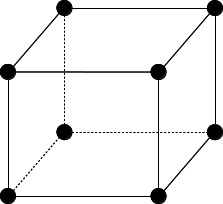
\includegraphics[scale=0.75]{images/Capitulo4/Hypercube2.jpg}
  \caption{Red distribuida}  
\label{fig:Hypercube} 
\end{figure}

En este trabajo de tesis, la confiabilidad se calculó por medio del siguiente modelo: $$R_{sys} = 1- [N (1 - e^{- \lambda t}]$$

Como se puede observar el modelo es similar al modelo de árboles binario. Como se pudo estudiar en la bibliografía, árboles binarios y redes hypercube presentan varias similitudes, incluso se emebebe árboles binarios en este tipo de red. La \textit{curva de confiabilidad} de esta red se la puede observar en la fgura 

\begin{figure}[H]
 \centering
 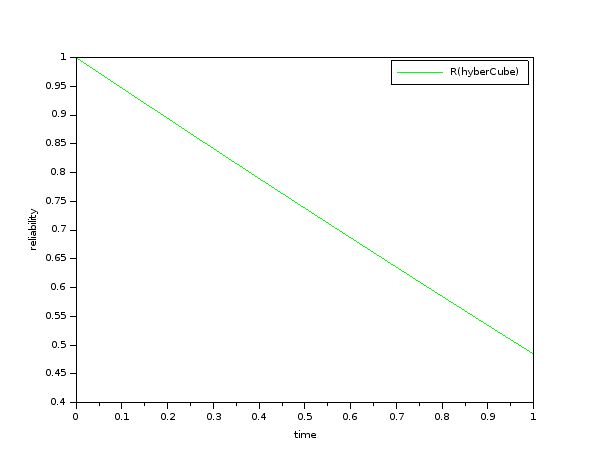
\includegraphics[scale=0.5]{images/Capitulo4/Reliability_Hypercube.png}
  \caption{Red distribuida}  
\label{fig:Reliability_Hypercube} 
\end{figure}

\section{Topología utilizada en la arquitectura a diseñar}

Teniendo en cuenta los modelos presentados anteriormente, se procede a realizar una comparación de las diferentes curvas. El resultado de esto, permitiré conocer de manera analítica qué topología presenta una mayor tolerancia a fallas a travez del tiempo. Además, teniendo en cuenta lo estudiado en el estado de la cuestión, se puede realizar una comparación conceptual de las tres topologías.

La aplicación de árboles binario podríar resultar una buena opción, ya que representa un desarrollo sencillo. En contraposición se puede indicar que existe un alto grado riesgo de que se produzca una falla en el nodo raíz y de su redundancia, lo cual pondría en peligro la misión. Así mismo, presenta otro punto negativo que se puede mencionar y es la gran cantidad de enlaces que esta necesita para mantener a todos los nodos de la red conectados.

Por otra parte, la red distribuída cuenta con la capacidad de distribuir el trabajo en todos sus nodos. Esto quiere decir, que si se produce una falla irrecuperable en cualquiera de sus nodos, la arquitectura podría continuar funcionando sin verse afectada por la ausencia de dicho nodo. Esto demanda un procesamiento computacional extra, y la necesidad de desarrollar algorimtos de ruteo especiales. Además, como punto negativo se puede mencionar que también, al igual que los árboles binarios, necesitan una gran cantidad de enlaces.

Por último, las topologías hypercube tiene un excelente respaldo teórico, exigen menor cantidad de enlaces, y pueden tolerar la falla de una gran cantidad de nodos (hasta el 50\% de los nodos). Su complejidad aumenta en gran medida, cuando se desarrollan arquitecturas de más dimensiones, sin embargo, esto aumenta su confiabilidad.

Como se mencionó en el primer párrafo, se realizó una comparación de módelos de confiabilidad de las tres topologías estudiadas. Se asumió que la distribución de la confiabilidad es exponencial, con una tasa de falla fija de 1/15, y se estudió su evolución en un rango $[0,1]t$. El resultado de esta comparación se la puede observar en la Figura \ref{fig:comparative_reliablities} y en la Tabla \ref{table_comprative_reliability}.

Se observa que tanto las redes distribuidas como la hypercube presenta una mayor confiabilidad a través del tiempo que  los árboles binarios. Si bien, las redes distribuidas y la hypercube tienen una curva similar, la primera presenta una mayor confiabilidad sostenida en el tiempo.

\begin{figure}[H]
 \centering
 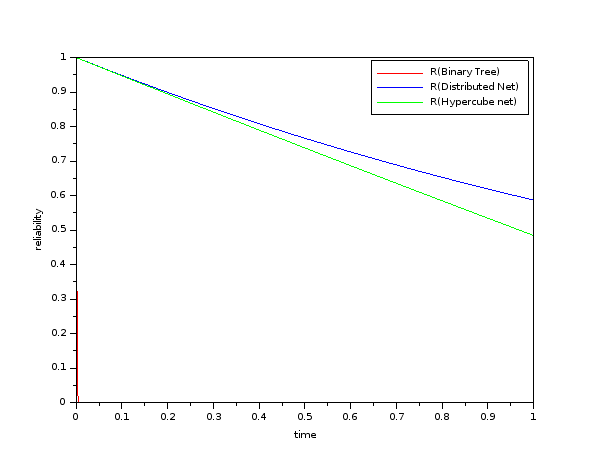
\includegraphics[scale=0.5]{images/Capitulo4/comparative_reliablities.png}
  \caption{Red distribuida}  
\label{fig:comparative_reliablities} 
\end{figure}

\begin{table}[H]
\centering
\caption{Comparación de confiabilidad de topologías}
\label{table_comprative_reliability}
\begin{tabular}{r|r|r|r|}
\cline{2-4}
\multicolumn{1}{l|}{} & \multicolumn{3}{c|}{Topologías de red} \\ \hline
\multicolumn{1}{|c|}{T} & \multicolumn{1}{c|}{Tree Net} & \multicolumn{1}{c|}{Distr Net} & \multicolumn{1}{c|}{Hyper Net} \\ \hline
\multicolumn{1}{|r|}{0} & 1 & 1 & 1 \\ \hline
\multicolumn{1}{|r|}{0.001} & 0.803766 & 0.999947 & 0.999947 \\ \hline
\multicolumn{1}{|r|}{0.002} & 0.64604 & 0.999893 & 0.999893 \\ \hline
\multicolumn{1}{|r|}{0.003} & 0.519265 & 0.99984 & 0.99984 \\ \hline
\multicolumn{1}{|r|}{0.004} & 0.417368 & 0.999787 & 0.999787 \\ \hline
\multicolumn{1}{|r|}{0.005} & 0.335466 & 0.999733 & 0.999733 \\ \hline
\multicolumn{1}{|r|}{...} & ... & ... & ... \\ \hline
\multicolumn{1}{|r|}{0.995} & 0 & 0.948317 & 0.947109 \\ \hline
\multicolumn{1}{|r|}{0.996} & 0 & 0.948266 & 0.947056 \\ \hline
\multicolumn{1}{|r|}{0.997} & 0 & 0.948216 & 0.947003 \\ \hline
\multicolumn{1}{|r|}{0.998} & 0 & 0.948165 & 0.94695 \\ \hline
\multicolumn{1}{|r|}{0.999} & 0 & 0.948115 & 0.946897 \\ \hline
\end{tabular}
\end{table}


Con esto se puede concluir que la topología que presenta un mayor grado de confiabilidad es la que responde a una filosofía distribuida (bajo las condiciones en las que fueron estudiadas). Por lo tanto, la arquitectura satelital, tolerante a fallas y basada en componentes COTS que se desarrolla en la presenta tesis se basa en una \textbf{topología distribuída} para interconectar los diferentes subsistemas. 

\section{Topología propuesta}
Sobre la base de los resultados presentados en \citep{Arias17} se puede establecer que la topoloǵia propuesta es la más adecuada para el desarrollo de una arquitectura tolerante a fallas como se presenta en la Figura \ref{fig:topo_propuesta}. En esta se puede observar que cada subsitema (térmico, power, telemetría, etc.) tiene su propia CPU controladora. Estas CPU se conectan a los nodos. 

\begin{figure}[h]
 \centering
 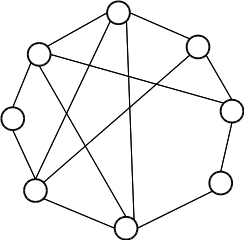
\includegraphics[scale=0.75]{images/Capitulo4/distributed_network.jpg}
  \caption{Red distribuida}  
\label{fig:topo_propuesta} 
\end{figure}

El modelo exige como requerimiento que cada nodo debe estar compuesto por una computadora (componente COTS) que es la encargada de realizar el procesamiento de las tareas. También, debe exitir un puente de comunicación entre la red y la CPU del subsistema. De este modo se hace frente a posibles fallas en la computadora del nodo. Esta conexión se observa en la Figura \ref{fig:conn_prop}

\begin{figure}[h]
 \centering
 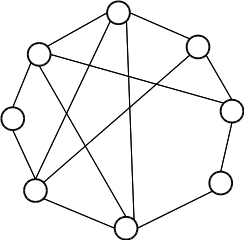
\includegraphics[scale=0.75]{images/Capitulo4/distributed_network.jpg}
 \caption{Red distribuida}  
\label{fig:conn_prop} 
\end{figure}




% section that talk about the comm protocol
\section{Protocolo de comunicación}
Como se estudió en el marco teórico, en una arquitectura
de comunicación, el protocolo CAN trabaja en las
capas inferiores del modelo de OSI. CAN propone cómo debe ser
el medio físico, y la manera de transmisión de las señales.
Además, preve cuál es la estrategia a utilizar  para sincronizar
la transmisión de datos sin nigún tipo de latencia, ni tampoco
colisiones de mensajes. Así, este protocolo permite que estos
sean envíados teniendo en cuenta sus prioridades, eliminando las colisiones, y
por lo tanto también, el tiempo de espera en la que los nodos se quedan
relegados cuando han tratado de enviar un mensaje al mismo tiempo.

Este protocolo no establece nada sobre ruteos de mensajes, tipos de mensajes y
tipos de datos, que a la hora de desarrollar una arquitectura de aviónica es
importante tener en cuenta esos detalles. Es necesario, que exista una
capa de servicios que facilite la comunicación entre aplicaciones de usuarios
de diferentes nodos, y la comunicción entre las aplicaciones de usuario
y el protocolo CAN (de bajo nivel) en sí.
Además, teniendo en cuenta los resultados obtenidos en las secciones
anteriores, se necesita además, diseñar un protocolo de comunicación
basado en redes distribuidos, y que a su vez, esté basado en CAN.

Por tales motivos, surge la necesidad
de diseñar un protocolo de comunicación basado en CAN, que se ``monte'' sobre
las capas superiores del modelo de referencia de OSI; y que permita
la distribución de las tareas y el procesamiento llevado a cabo
por los nodos. 

El protocolo CANae se encuentra en su primera versión 0.1 Alpha. Esto hace
referencia a que en esta instancia de trabajo se tratar de comprender
el problema y llevar a cabo un diseño preliminar de protocolo. De esta
manera se podrá extraer, tanto puntos positivos, como puntos negativos; o
más bien fortalezas y debilidades del stack de servicios que brinda CANae.

CANae actúa en la capa de aplicación del modelo de referencia de OSI. CANae
divide esta capa en dos subcapas:
\begin{itemize}
\item CANae Application Layer
\item CANae High Application layer
\end{itemize}

\begin{figure}[h!]
 \centering
 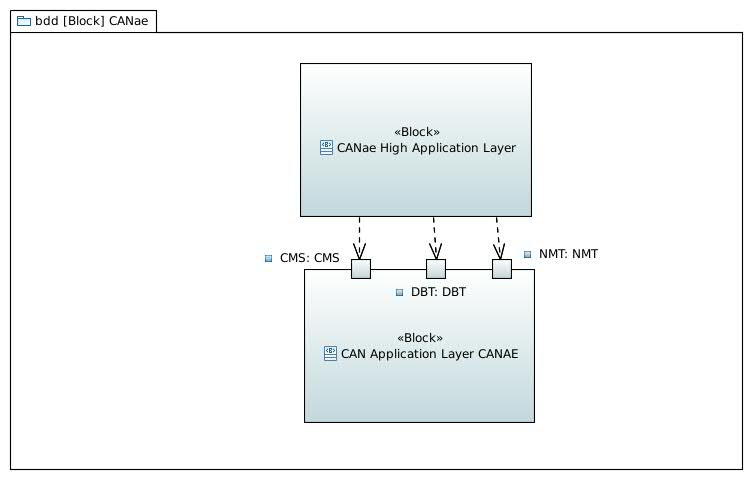
\includegraphics[scale=0.5]{images/Secciones/AppendixA/CANAE.JPG}
  \caption{Estructura de la capa de aplicación de CANae en alto nivel}
\label{fig:CANAEC4}
\end{figure}

Esto puede observar se en la Figura \ref{CANAEC4}. En el gráfico se observa que
la CANae application Layer, cuenta con 3 interfaces:n
\begin{itemize}
\item \textbf{CMS}: ofrece un ambiente orientado a objecto para diseñar aplica-
ciones de usuario. Esta entidad ofrece variables y eventos, y específica como un módulo pude acceder a
las interfaces de CAN.
\item \textbf{NMT}: ofrece un ambiente orientado a objetos para permitir que un módulo (el
NMT Master) se ocupe de la inicialización y posibles fallas de otros módulos (NMT Slaves).
\item \textbf{DBT}: ofrece el servicio para distribuir dinámicamente el identificador de para los diferentes nodos.
\end{itemize}
Debe destacarse que, el servicio CMS ofrece un ambiente orientado a objeto  para diseñar
aplicaciones de usuario, es decir, que ofrece la posibilidad de modelar el
comportamiento del sistema en forma de objeto. Este servicio ofrece la posibilidad
de crear variables y eventos, según las necesidades de los usuariosm que son
utilizadas para diseñar y especificar como la funcionalidad de un módulo puede
acceder a las interfaces de bajo nivel de CAN. Esto propone un grado de innovación
al tratar al protocolo, a los datos, mensajes y eventos como objetos, permitiendo así
un modelado orientado a objetos. Por tal motivo, este protocolo fue modelado
con SysML (System Modeling Language).
Para mayor detalle de estas interfaces se debe consultar en el apéndice \ref{Appendix:A}.

Agregando, dentro de esta capa existen dos entidades que juegan un papel importante
(consultar apéndice \ref{Appendix:A}) las cuales son:
\begin{itemize}
\item \textbf{Gestor de mensajes}: este se encarga de gestionar los mensajes que son enviados y recibidos desde la red.
Esta entidad debe ser capaz de determinar si el mensajes contiene datos o eventos. Trabaja en conjunto
con el CMS.
\item \textbf{Gestor de nodo}: esta entidad se encarga de llevar el control de los nodos existenten en la red. En este
nodo se encuentra la tabla de ruteo primario y secundario necesarios para la correcta comunicación.
\end{itemize}

La subcapa denominada CAN High Application Layer tiene una función más del lado de la gestión de nodos y tareas.
En esta capa se desarrollan los algoritmos necesarios para realizar el ruteo y la reconfiguración de la red ante
fallas, por lo tanto en la High Application Layer se debe implementar la FDIR. El protocolo no define ninún
algoritmo de ruteo, por lo que queda para el usuario la definición de los algoritmos.
El protocolo  recomienda desarrollar dos algoritmos, el primario y el secundario.
Para aumentar la tolerancia a fallas se pueden desarrollar más algoritmos
secundarios, y el switch entre algoritmos, puede depender de medidas de perfomance.

Así, queda conformada el protocolo de comunicación CANae como uno de los
principales productos de este trabajo de tesis. 


\vspace{1cm}
\noindent\rule{\textwidth}{2pt}

\textbf{\Large{Resúmen}}

En este capítulo se llevó a cabo un estudio de tres tipos de topologías tolerantes
a fallas que fueron candidatas a ser utilizadas como base en la
arquitectura que se diseñó en este trabajo de tesis. 

Teniendo en cuenta los modelos que se han desarrollado en este capítulo se compararon las diferentes curvas de confiabilidad. El resultado de esto, permitió conocer de manera analítica qué topología presenta una mayor tolerancia a fallas a través del tiempo.

Se asumió que la distribución de la confiabilidad es exponencial, con una tasa de falla fija de 1/15, y se estudió su evolución en un rango $[0,1]t$. El resultado de esta comparación se la puede observar en la Figura \ref{fig:comparative_reliablities} y en la Tabla \ref{table_comprative_reliability}.

Se observa que tanto las redes distribuidas como la hypercube presentan una mayor confiabilidad a través del tiempo que  los árboles binarios. Si bien, las redes distribuidas y la hypercube tienen una curva similar, la primera presenta una mayor confiabilidad sostenida en el tiempo.

Así en este capítulo se llegó a la conclusión de que la topología que presenta un mayor grado de
confiabilidad es la que responde a una filosofía distribuida.  Por lo tanto, la arquitectura satelital, tolerante a fallas y basada en componentes COTS que se desarrolla en la presenta tesis se basa en una \textbf{topología distribuida} para interconectar los diferentes subsistemas.

\chapter{Arquitectura propuesta}
\section{Introducción}

La arquitectura propuesta se centra en la comunicación de la aviónica de un
vehículo espacial, con la característica de que sus componentes (nodos) son
de baja confiabilidad (se piensa en la utilización de compoentes COTS)
por lo tanto, es necesario que esta arquitectura sea tolerante a fallas. En este
trabajo el protocolo de comunicación (tolerante a fallas) propuesto,
se encuentra en las capas superiores del modelo de referencia OSI\footnote{ISO/IEC 7498-1 - Open System Interconnection}


Aquí hago la propuesta de la arquitectura.

El capítulo estará dividido en

\begin{itemize}
\item Arbol de requerimientos
\item Diseño estructural (Diagramas de bloques, bloques internos)
\item Diseño dinámico (Diagramas de secuencia, interacción, maquina de estados,)
  
\end{itemize}

\section{Árbol de requrimientos}
A continuación se detallas los requerimientos que van a guiar el diseño y
desarrollo de la propuesta de arquitectura de aviónica tolerantes a fallas
basada en componentes \ac{COTS} para satélites. En la Figura
\ref{fig:DiagramaRequerimientos} y en la Tabla \ref{table:Requerimientos} se pueden
observar los requerimientos. 

\begin{figure}[h!]
 \centering
 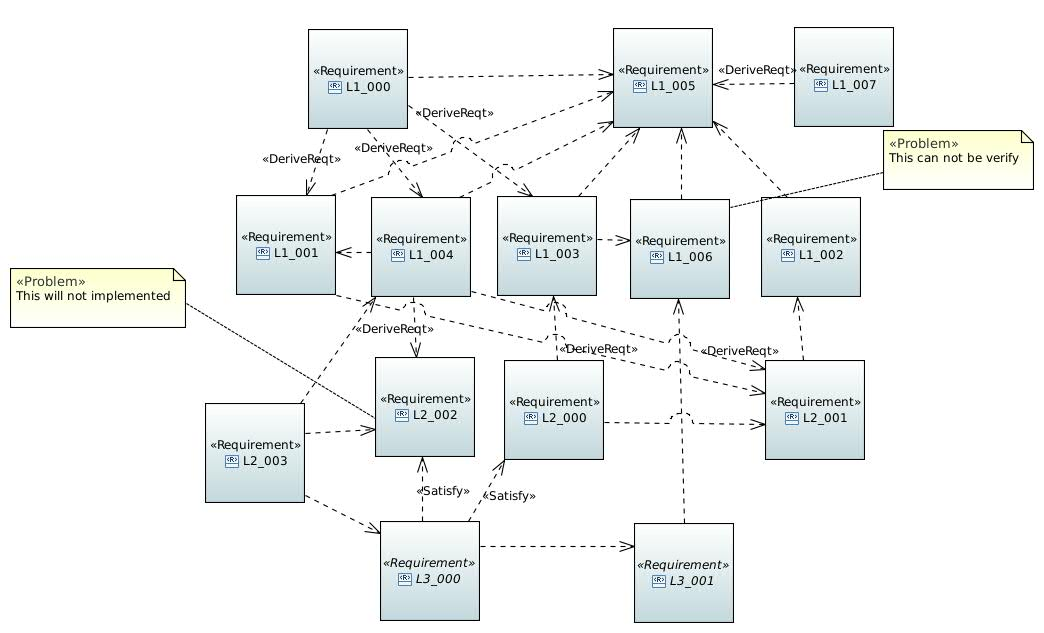
\includegraphics[scale=0.4]{images/Capitulo5/Diagrama_de_Requerimientos.JPG}
  \caption{Diagrama de requerimientos de la arquitectura propuesta}
\label{fig:DiagramaRequerimientos}
\end{figure} 

% \begin{sidewaystable}[]
\begin{table}[]
\small
\centering
\caption{Tabla de Requerimientos}
\label{table:Requerimientos}
%\resizebox{\textwidth}{!}{%
\begin{tabular}{|l|l|l|p{7cm}|p{2cm}|}
\hline
\multicolumn{1}{|c|}{\textbf{}} & \multicolumn{1}{c|}{\textbf{ID}} & \multicolumn{1}{c|}{\textbf{Name}} & \multicolumn{1}{c|}{\textbf{Detail}} & \multicolumn{1}{c|}{\textbf{Kind of Requirements}} \\ \hline
0 & L1\_001 & L1\_001 & The architecture components shall be Components Off-The-Shelf category & Constraint \\ \hline
1 & L2\_000 & L2\_000 & The architecture shall be reconfigurate when a node fail. & Funcional \\ \hline
2 & L2\_001 & L2\_001 & Each subsystem shall represented for a Components Off-The-Shelf & Constraint \\ \hline
3 & L1\_000 & L1\_000 & Shall be develop an avionics architecture for spacecraft using Components Off-The-Shelf & Constraint \\ \hline
4 & L1\_002 & L1\_002 & The architecture shall have at least 6 subsystems & Constraint \\ \hline
5 & L1\_003 & L1\_003 & The architecture shall have fault tolerance techniques to assurance the the mission life & No funcional \\ \hline
6 & L1\_004 & L1\_004 & The main bus to interconnect components shall be the Controller Area Network Bus developed for Bosch & Constraint \\ \hline
7 & L1\_005 & L1\_005 & The architecture shall be sufficient to make a master degree thesis & No funcional \\ \hline
8 & L2\_002 & L2\_002 & The architecture shall implements a based Controller Area Netowork protocol to intercommunicate the components & Funcional \\ \hline
9 & L3\_000 & L3\_000 & The intercomunication beteween nodes shall used a Controller Area Netowork protocol based developed in the master degree theis. & Constraint\\ \hline
10 & L1\_006 & L1\_006 & The architecture shall ssurance at least 10 years mission life & No funcional \\ \hline
11 & L3\_001 & L3\_001 & The architecture shall use the distributed network philosophy & Constraint \\ \hline
12 & L1\_007 & L1\_007 & The thesis shall be finished in 1 year & Constraint \\ \hline
13 & L2\_003 & L2\_003 & The nodes shall send and receive message from any nodes connected to the architecture. & Funcional \\ \hline
\end{tabular}%
%}
\end{table}
% \end{sidewaystable}

A continuación se explica cada uno de los requerimientos:
\begin{itemize}
\item\textbf{L1\_000}: Este es el objetivo principal de la presente tesis:
  desarrollar una arquitectura de aviónica tolerante a fallas basada en
  componentes COTS para vehículos espaciales.
\item\textbf{L1\_001}: El principal requerimiento de este trabajo de tesis,
  es desarrollar una arquitectura basada en componentes COTS, lo cual agrega un
  grado importante de innovación tecnológica y complejidad, siendo de especial
  interés para INVAP trabajar con estos tipos de componentes.
\item\textbf{L1\_002}: Este requerimiento hace referencia que se debe asegurar
  el correcto funcionamiento de la arquitectura con una cantidad de al menos
  6 subsistemas.
\item\textbf{L1\_003}: Este requerimiento exige que la arquitectura sea
  tolerante a fallas para así poder sastifacer el requerimiento \textbf{L1\_006}.
\item\textbf{L1\_004}: Este requerimiento (constraint) indica que se debe pensar
  la arquitectura para ser utilizada con el bus CAN de Bosch. Este requerimiento
  es de interés par INVAP.
\item\textbf{L1\_005}: Este requerimiento indica que la arquitectura que se
  desarrolle debe ser sufiencite para lograr terminar una tesis de maestría. Por
  el diseño y desarrollo debe ser solo el suficiente y necesario para cumplir
  con el presente trabajo.
\item\textbf{L1\_006}: Este requerimiento indica que debe asegurarse que la
  arquitectura sea lo suficientemente robusta como para asegurar el el tiempo de
  vida de la misión de 10 años como mínimo. Existe un \textbf{problema} con este
  requerimiento, y es que para los alcances de esta tesis, será imposible
  verificar si se cumple con este requerimiento.
\item\textbf{L1\_007}: Este requerimiento indica que el trabajo de tesis tiene
  que ser finalizado en menos de un año. Esto tiene relación con el
  requerimiento \textbf{L1\_005} debido a que no se logrará alcanzar el detalle
  necesario para lograr la correcta implementación, verifación y validación de
  la arquitectura.
\item\textbf{L2\_000}: Este requerimiento exige que la arquitectura pueda
  reconfigurarse cuando un nodo falle.
\item\textbf{L2\_001}: Este requerimiento indica que para esta instancia de
  trabajo cada subsistema será tratado como un nodo dentro de la arquitectura.
\item\textbf{L2\_002}: Este requerimiento indica que se debe utilizar dentro de
  la arquitectura un protocolo de comunicación basado en el Bus CAN de Bosch.
\item\textbf{L2\_003}: Este requerimiento asegura que los nodos deben poder enviar
  y recibir mensajes de cualquier otro nodo conectado a la red CANae.
\item\textbf{L3\_000}: Este requerimiento indica que el protocolo de
  comunicación utilizado en esta arquitectura debe estar basado en el
  el protocolo CAN. Este protocolo fue desarrollado en el presente
  trabajo de tesis bajo el nombre de CANae 0.1 Alpha (Vease: Apéndice \ref{Appendix:A}).
\item\textbf{L3\_001}: Este requerimiento exige la utilización de una
  filosofía de red distribuída para su diseño y desarrollo.
\end{itemize}

\section{Casos de Uso}
A continuación se muestra el diagrama de Casos de Uso para la arquitectura propuesta.
El diagrama de Casos de Uso tiene como propósito explicar de manera general
el comportamiento a nivel de sistema de la arquitectura propuesta.
Los actores identificadores para esta arquitectura son los diferentes
subsistemas que se conectan a la red a través de los nodos.
Los subsistemas interactúan con el nodo a través de
la aplicación de usuario, es decir se encuentra asociados.
Se puede observar en la Figura \ref{fig:DiagramaCUArqPropuestaGENERAL}
que de forma general existen tres casos de usos que comprenden el comportamiento
general de la arquitectura. Se tiene \textit{Enviar mensaje} y \textit{Recibir
  Mensaje} los cuales son básicos para cualquier arquitectura de comunicación. A
esto se le agrega el caso de uso de \textit{FDIR} que es el agregado que se le
hace en este trabajo de tesis a través del protocolo de comunicación desarrollado
denominado CANae (Ver apéndice \ref{Appendix:A}). Debe aclararse que en 
la Figura \ref{fig:DiagramaCUArqPropuestaGENERAL}
aparece un resumen de los Actores intereactuando con el sistema. 

\begin{figure}[h!]
 \centering
 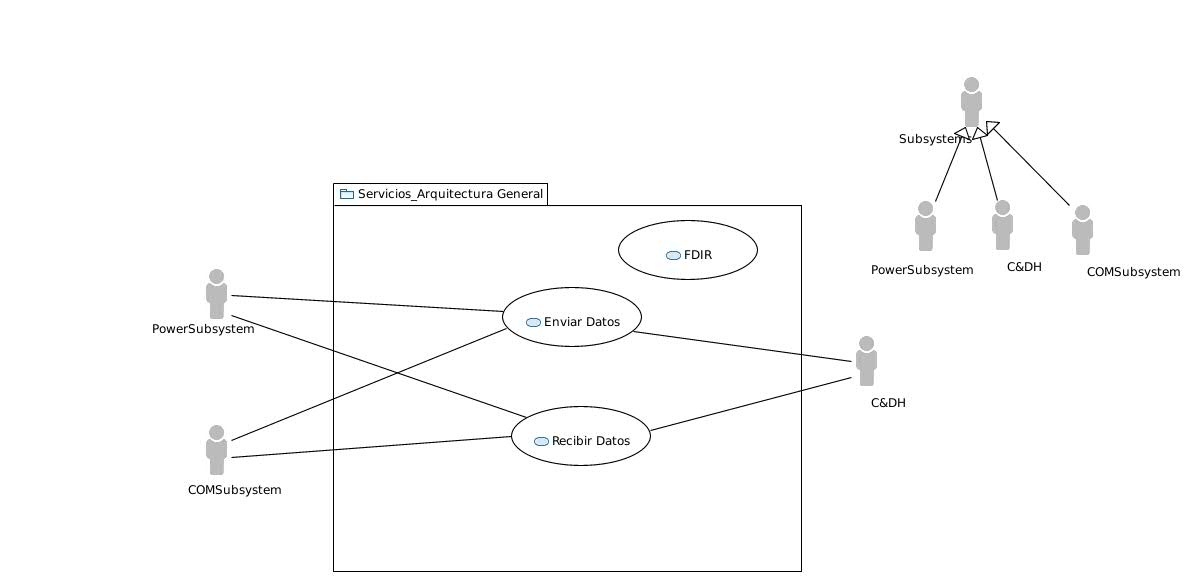
\includegraphics[scale=0.4]{images/Capitulo5/Arq_General.JPG}
  \caption{Diagrama de Casos de Uso General de la arquitectura Propuesta}
\label{fig:DiagramaCUArqPropuestaGENERAL}
\end{figure} 

De manera más detallada en la Figura \ref{fig:DiagramaCUArqPropuesta} se
observa un diagrama de casos de uso explayado. En este se pueden observar su
comportamiento.

\begin{figure}[h!]
 \centering
 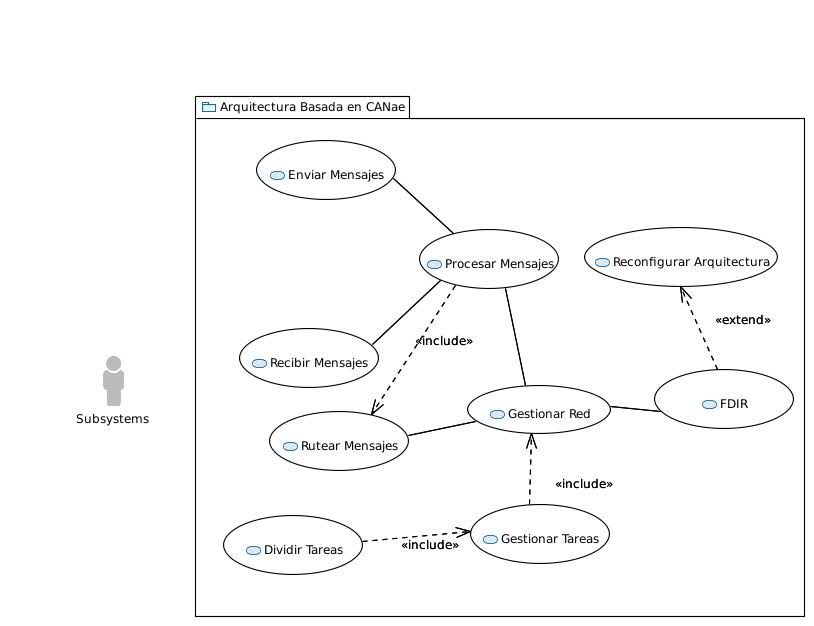
\includegraphics[scale=0.6]{images/Capitulo5/Caso_de_Uso_Arquitectura.JPG}
  \caption{Diagrama de Casos de Uso de arquitectura propuesta}
\label{fig:DiagramaCUArqPropuesta}
\end{figure} 

Le especifcación de los casos de usos se describen en \ref{Appendix:UseCase}.
Como se puede observar en la Figura \ref{fig:DiagramaCUArqPropuesta}
el sistema tiene 9 casos de uso.

Los casos de uso de \textit{Enviar Mensaje} y \textit{Recibir Mensaje} denota la
capacidad de la arquitectura de enviar y recibir mensajes (Data Frames de
CANae) desde y hacia las aplicaciones de usuario. Cuando una aplicación
necesita enviar un mensaje, estos deben primer pasar por el caso de uso
\textit{Procesar Mensaje} este es el encargado de empaquetar los mensajes.
También en este caso de uso se encuentra el caso de uso \textit{Rutear
  Mensaje}.

El caso de uso \textit{Rutear Mensaje} se encarga de aplicar los algoritmos
necesarios para lograr entregar el mensaje de una manera eficiente, siguiendo
la tabla de ruteo del CANae. Para esto se basa del caso de uso \texit{Gestionar
  Red}.

El caso de uso \texit{Gestionar Tareas} y \texit{Dividr Tareas} se encarga de
de conocer (periódicamente) el estado de la red y de sus nodos. Con esto puede
decidir cómo se reparten las tareas de una manera eficiente, siguiendo
la filosofía de arquitectura distribuída.

Por último tenemos el caso de uso \textit{FDIR} que hace referencia a la
Detección, Aislación, y Recuperación del sistema ante fallas. Debido a la
complejidad de esto, no se lo desarrolla a esta caso de uso en este trabajo.
El cual queda para \textbf{trabajos futuros}\ref{chap:TrabajosFuturos}. En este
caso de uso se encuentra el \textit{Reconfigurar Arquitectura}. Este es una
algoritmo del \ac{FDIR} que cuando se produce una falla en el algunos de los
nodos, la red se tiene que reconfigurar, para lograr continuar funcionando,
aún cuando haya nodos inactivos. Esto le brindaría a la arquitectura una grado
más de tolerancia a fallas. 

% talk about structural design
\section{Diseño Estructural}
gil


% talk about behavorial design
\section{Modelo dinámico}\label{sec:modelo_dinamico}
En esta sección se modelará el comportamiento de la arquitectura.
A diferencia de lo modelos  que se estudió en la sección anterior (diagramas
de bloques, diagrama de bloques internos) que hacen referencia al
\textit{qué} del sistema, en el modelado del comportamiento se
hace referencia al \textit{cómo} del sistema. Este \textit{cómo}
es descripto por el modelado del comportamiento dentro del
sistema \citep{HoltPery}.

En esta sección se verán  3 diferentes niveles de abstracción
de los modelos de comportamiento del sistema. En primer lugar, el
nivel más alto de abstracción es la máquina de estado, que considera la
interacción entre bloques. El siguiente diagrama que se verá es
el diagrama de secuencia, el cual pone en manifiesto los diferentes
mensajes que son enviadas entre las entidades. Y por último, se
desarrolla el diagrama de actividades, siendo este el nivel
más bajo de abstracción del modelado del comportamiento del sistema.

\subsection{Máquina de estado}
En esta subsección se describe el ciclo de vida de los
bloques que conforman la arquitectura. En resúmen, lo que se
pretende demostrar, es el comportamiento de los objetos de la
arquitectura.

En la Figura \ref{fig:StateMachineArqCompleta} se presenta la
máquina de estado de la arquitectura completa.  En esta se
puede observar todos los estados por los cuales la arquitectura
debe recorrer.

\begin{figure}[h!]
 \centering
 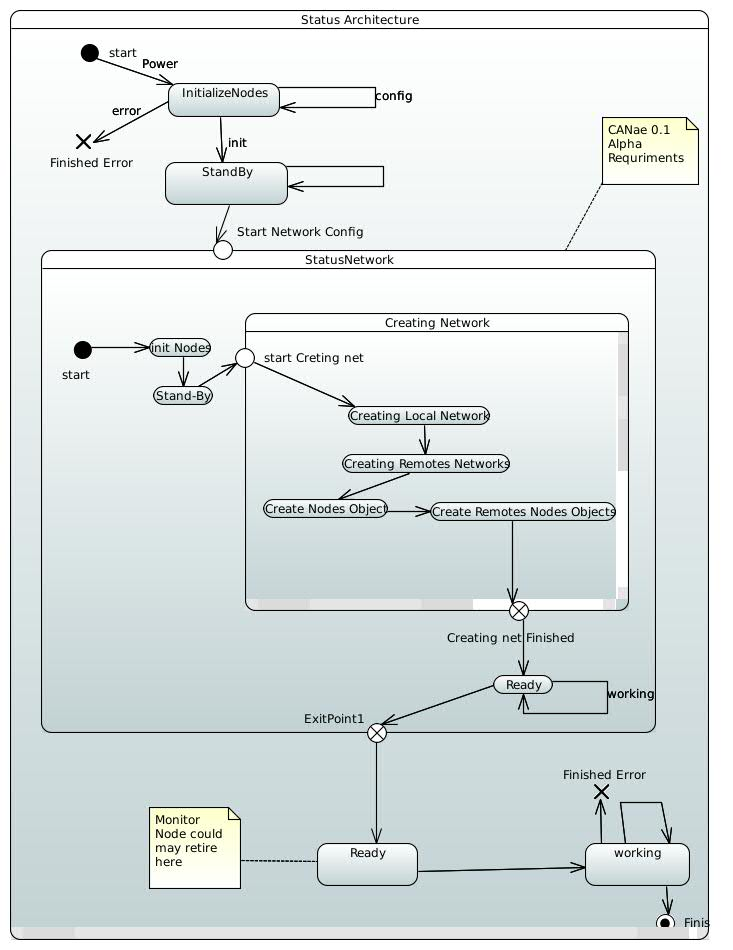
\includegraphics[scale=0.4]{images/Capitulo5/StateMachineArqCompleta.JPG}
  \caption{Máquina de estado de la arquitectura completa}
\label{fig:StateMachineArqCompleta}
\end{figure}

A continuación se procede a explicar la máquina de estado. Todo
inicia en el momento en el que la red es alimentada (eléctricamente)
siguiendo los protocolos de CAN \citep{can-ciaWEB}. En primer lugar, la
red pasa a un estdo de inicialización de los nodos, en los cuales, estos
son alimentados, se encienden, y comienzan con todos los procedimientos
normales de cualquier sistema embebido. Los cuales son Booteo, checkeo del
funcionamiento y del estado de salud del propio \ac{HW} y los \ac{HW}
conectados a él. Esto incluye la iniciación, del protocolo CANae como
un stack más del servicio del sistema operativo o sistema embebido
que gobierna a cada uno de los nodos. Esto se observa en la Figura
\ref{fig:StateMacineInitNodes}.

\begin{figure}[h!]
 \centering
 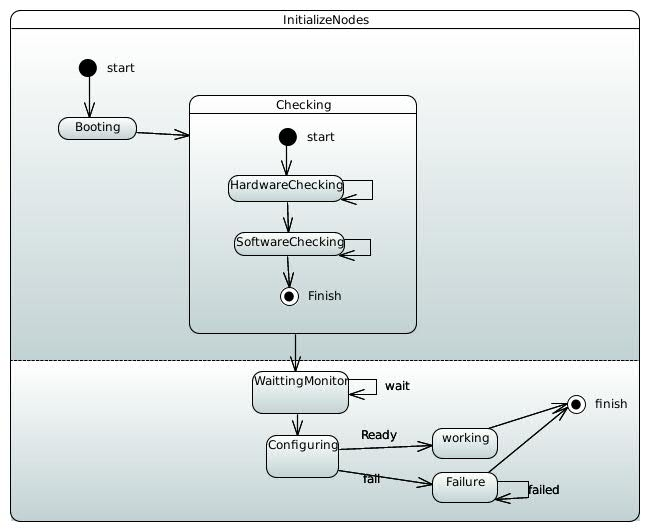
\includegraphics[scale=0.4]{images/Capitulo5/InitializeNodes.JPG}
  \caption{Máquina de estado de los nodos.}
\label{fig:StateMacineInitNodes}
\end{figure}

Una vez que todos los nodos se encuentran inicializados, y la red se encuentra
estable\footnote{Defínase como estable, la situación en la que el
  protocolo CANae se inicializó correctamente y está listo para pasar
  a la segunda etapa.}, la arquitectra pasa a un estado de Stand-By.
En este estado, la arquitectura espera por la orden del nodo monitor
para comenzar a configurar la red. Aquí se sigue lo indicado en el
protocolo CANae (Véase apéndice \ref{Appendix:A}). En primer lugar,
se crean las instancias de red localmente. Luego,  el nodo monitor
coordina la creación de las instancias de red remota. Luego se crean
los objetos nodos tanto locales como remotos. Estas actividades
son necesarias para lograr establecer una correcta comunicación
entre nodos utilizando el protocolo CANae (Versión 0.1 Alpha).

Una vez finalizada la creación de la red, la arquitectura completa
pasa a un estado Ready, donde el nodo monitor ya puede ser retirado.
Luego, la arquitectura ignora el nodo monitor (Si todavía se encuentra
conectado) y ya puede comenzar a trabajar normalmente.

\subsection{Diagrama de secuencia}
A continuación se muestra los diagramas de secuencias, para entender
cuál es el comportamiento de la arquitectura, en un grado
de abstracción menor.

En la Figura \ref{fig:SecInitArq} se puede observar como en
el momento de alimentar (eléctricamente) a los nodos, este comienza,
en primer lugar, a ejecutar el boostrap. Este bootea al
sistema operativo (o sistema embebido según sea la tecnología
que se utilice). Una vez que el sistema operativo es cargado se
deben ejecutar (preferentemente) dos tipos diferentes de chequeos:
\begin{itemize}
\item Hardware Check
\item Software Check
\end{itemize}

\begin{figure}[h!]
 \centering
 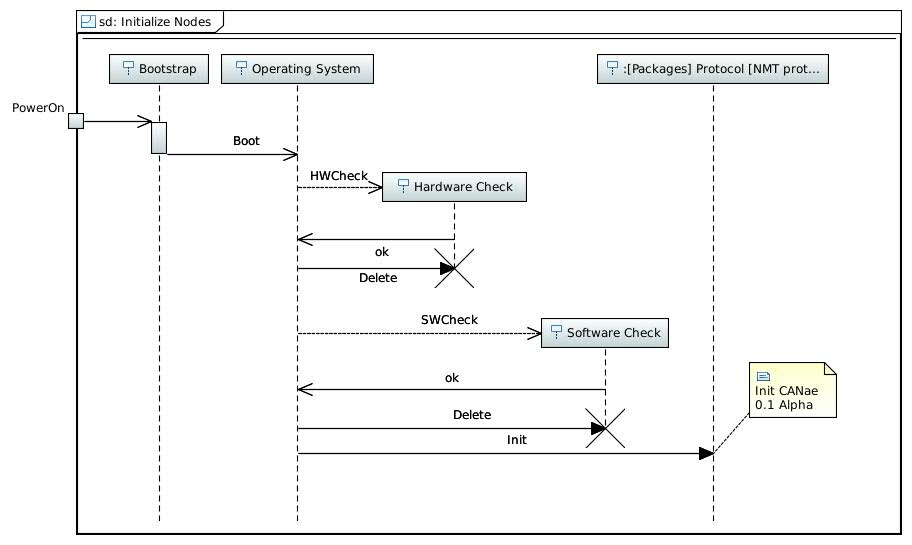
\includegraphics[scale=0.4]{images/Capitulo5/SecuenciaIInitNodes.JPG}
  \caption{Diagrama de secuencia del inicio de la arquitectura.}
\label{fig:SecInitArq}
\end{figure}

Estos son dos piezas de código. El primero tiene como tarea principal
chequear el estado de salud de los equipos de hardware, tanto
del propio nodo, como así también del subsistema que tiene más proximo.
Como se expuso en la subsección \ref{subsec:bridge} cada nodo tiene
próximo a él (físicamente hablando) un subsistema (con su computadora
de vuelo). Por lo tanto el nodo se debe encargar de chequear el
estado de salud de los diferentes componetes de ese subsistema. El
segundo chequeo, se ocupa de verificar el estado de salud del software
tanto del nodo, como del subsistema más próximo.

Luego de que los chequeos se hayan resuelto exitosamente se crea una
instancia del protocolo CANae y da inicio a su servicio NMT. Este
servicio se puede observar en la Figura \ref{fig:NMTC5}. En primer lugar
se debe esperar que el nodo monitor esté inicializado, y este les
envía un mensaje de \textit{crete\_remote\_network()} a todos los
nodos conectados a la arquitectura. Este mensaje llega al NMT del
protocolo de CANae de todos los nodos.

\begin{figure}[h!]
 \centering
 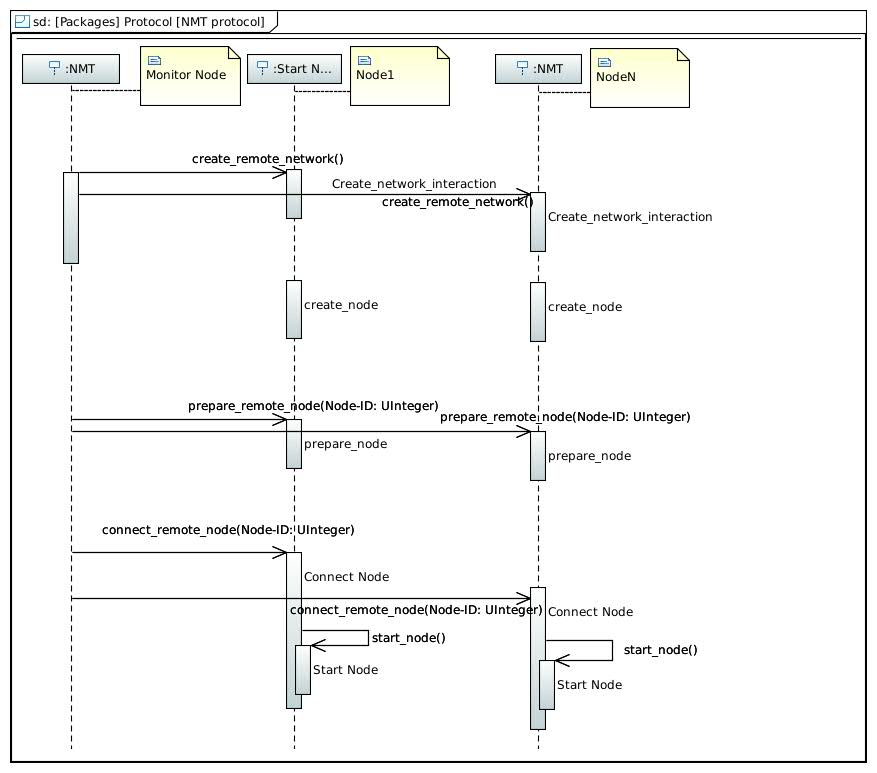
\includegraphics[scale=0.4]{images/Secciones/AppendixA/Protocol_NMT.JPG}
  \caption{Diagrama de secuencia de CA}
\label{fig:NMTC5}
\end{figure}

Luego, siguiendo el protocolo de CANae, cada nodo crea su instancia de
nodo. Esto puede observarse en la Figura \ref{fig:CreateNodeNMTC5}.
El objeto de \textit{CANAppLayerController} envía el mensaje \textit{
  create\_node()} al \textit{NodeManagement} de \textit{create\_newtork\_object()} con el objetivo de crear una instancia local de la red.


\begin{figure}[h!]
 \centering
 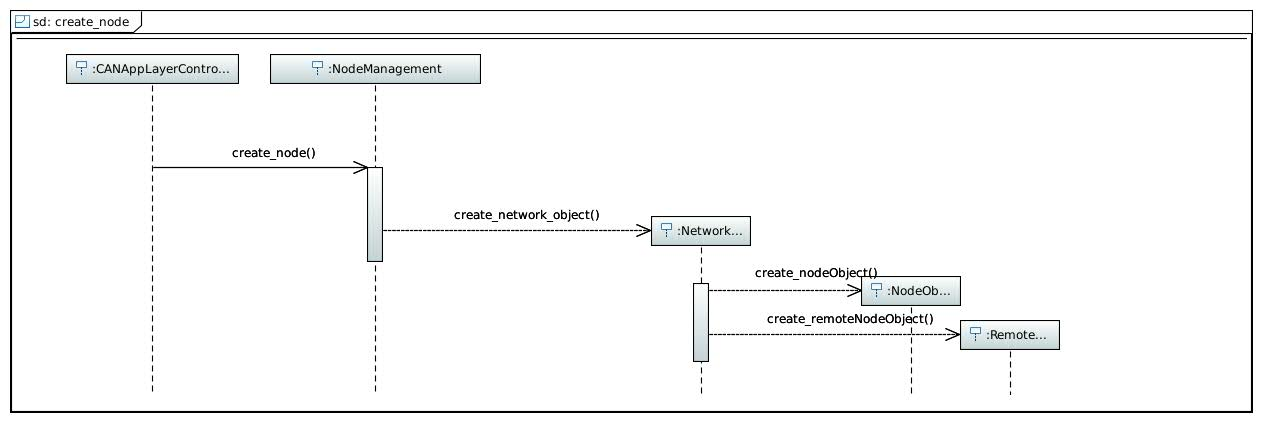
\includegraphics[scale=0.4]{images/Secciones/AppendixA/create_node.JPG}
  \caption{Crear Objecto Red, Objeto Nodo y Objeto Nodo Remoto}
  \label{fig:CreateNodeNMTC5}
\end{figure}

Luego el nodo monitor envía el mensaje \textit{prepare\_remote\_node()}.
El protocolo CANae preve los pasos que se muestran en la Figura
\ref{fig:PrepareNodeC5}

\begin{figure}[h!]
 \centering
 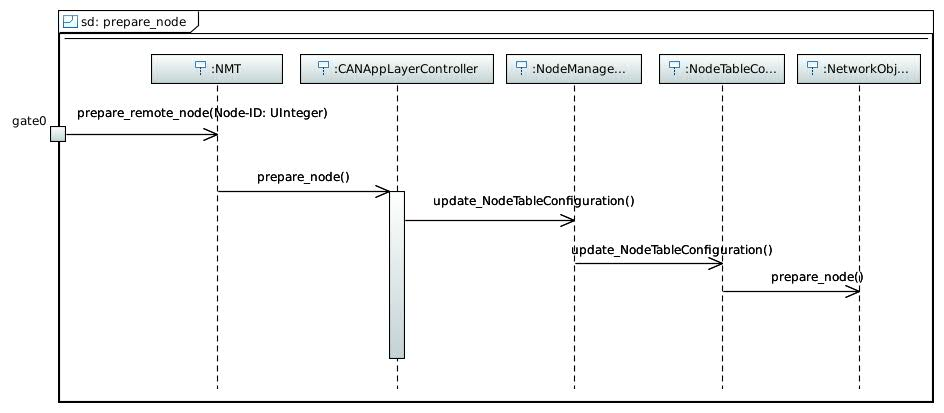
\includegraphics[scale=0.4]{images/Secciones/AppendixA/PrepareNode.JPG}
  \caption{Preparar nodo para la conexión a la red CAN}
  \label{fig:PrepareNodeC5}
\end{figure}

Por último, se conectan todo los nodos a la red, para lo cual deben
actualizar el \textit{Node Table Configuration}, y finalmente ya
pueden comenzar a comunicarse. Esto se observan en las Figuras
\ref{fig:PrepareNodeC5} y \ref{fig:ConnectNodeC5}

\begin{figure}[h!]
 \centering
 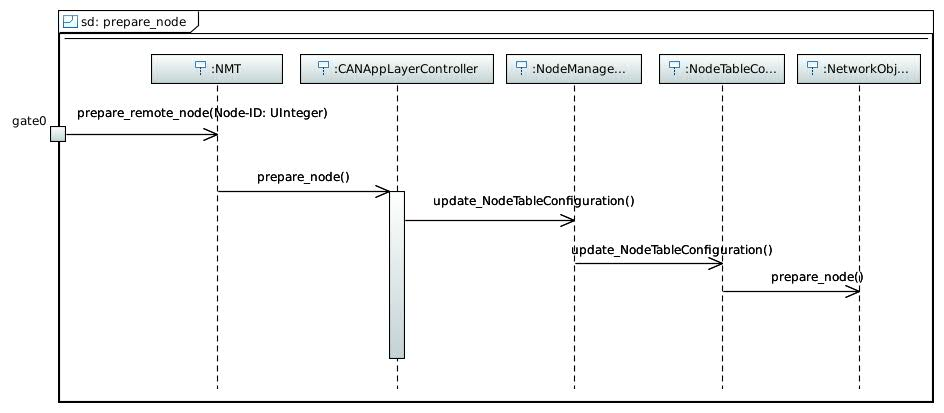
\includegraphics[scale=0.4]{images/Secciones/AppendixA/PrepareNode.JPG}
  \caption{Preparar nodo para la conexión a la red CAN}
  \label{fig:PrepareNodeC5}
\end{figure}

\begin{figure}[h!]
 \centering
 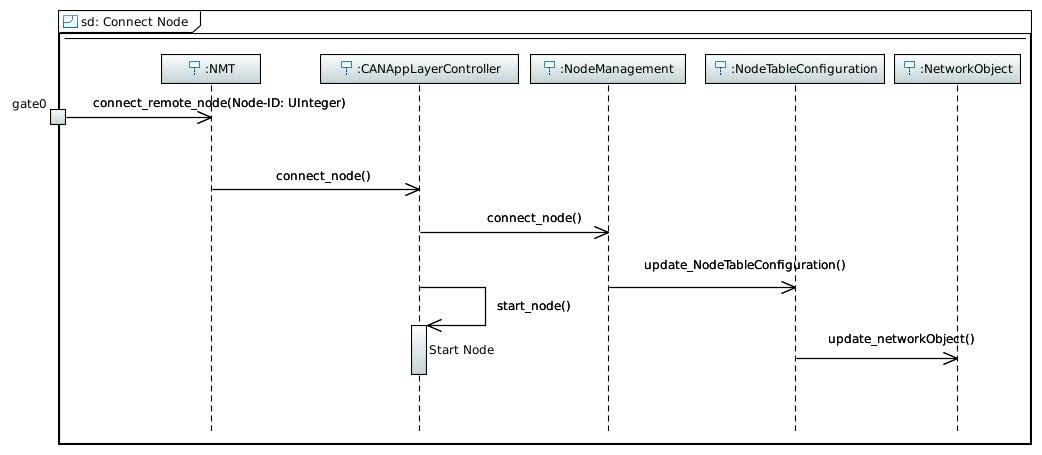
\includegraphics[scale=0.4]{images/Secciones/AppendixA/connect_node.JPG}
  \caption{Conectar el nodo a la red CAN}
  \label{fig:ConnectNodeC5}
\end{figure}

\subsection{Diagrama de actividades}
En esta subsección se verá algunos diagramas de actividad para modelar
el comportamiento de la arquitectura propuesta. Los diagramas de actividades
comúnmente son utilizados, generalmente, para describir el comportamiento
a muy bajo nivel (a nivel de componentes), en otras palabras para modelar
procesos, mientras que los diagramas de secuencia muestran el comportamiento
entre elementos, y las máquinas de estados  muestran el comportamiento
dentro de los elementos \citep{HoltPery}.

En la Figura \ref{fig:initNodes} se puede observar el proceso, en detalle,
del inicio de los nodos. Todo comienza cuando se alimenta (eléctricamente)
el nodo. En primer lugar, se ejecuta (como ocurre normalmente) el bootstrap,
este bootea al sistema operativo o al sistema embebido (dependiendo de como
se implemente). Los siguientes pasos son los esperados para cualquier sistema
espacial. Se chequea el \ac{HW} propio del nodo, se chequea memoria y componentes.
Luego, se chequea el estado de salud del subsistema. Para ello, se puede pedir
el chequeo a la CPU del subsistema, y este a vez, chequea los componentes
propios del subsistema.

Con estos pasos se puede obtener el Houskeeping (HK) tanto de \ac{HW} propio del nodo
como del subsistema. Este HK es recibido por el sistema operativo
(o sistema embebido), y se comienza a hacer un chequeo del lado del
software. Esto significa que se pueden realizar cualquier tipo de actividad
para chequear que las tareas (o procesos) se ejecuten correctamente.

Para finalizar, el sistema operativo crea una instancia del stack de servicio de
comunicación, dónde se encuentra el protocolo de comunicación CANae.

Debe observarse que el chequeo de \ac{HW} tanto propio como el del
subsistema se encuentra dentro de lo que se denomina \textit{zona interrumpible},
esto significa que si se da alguna \textit{Falla} (Failure en la Figura), debe
activarse el sistema FDIR del nodo. Este, lo que busca en primer lugar,
es detectar la falla, dónde se produjo y por qué. Luego, el sistema trata de
aislar la falla para que no afecte a ningún otro componente. Por último, el
sistema hará el intento de recuperarse de la falla, en el caso de que se
recupere correctamente, se regresa la tarea de chequeo, para
llevar a cabo estas actividades nuevamente; en caso contrario se termina la actividad.

\begin{figure}[h!]
 \centering
 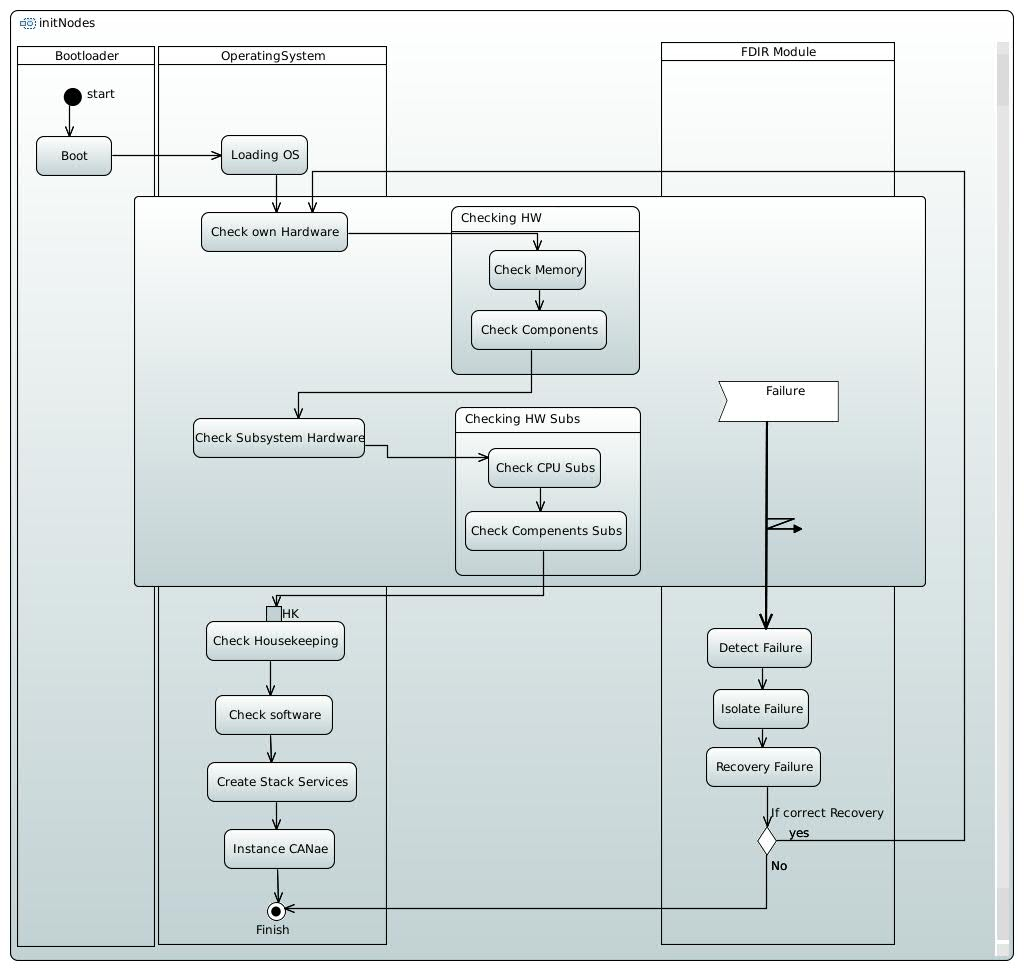
\includegraphics[scale=0.4]{images/Capitulo5/initNodes.JPG}
  \caption{Diagrama de actividades del inicio de nodos}
  \label{fig:initNodes}
\end{figure}

Otra parte importante a modelar de la arquitectura propuesta, es el momento
de la creación de la red CANae. Como se mencionó anteriormente el protocolo
CANae (Véase apéndice \ref{Appendix:A}) requiere de la existencia de un nodo monitor
para coordinar la creación de la red CANae. Este modelo se puede observar
en la Figura \ref{fig:NodeMonitor}.

El nodo monitor inicia la creación y configuración del nodo enviando la
señal \textit{create\_remote\_network()} a todos los nodos conectados a la
red. Cada nodo que recibe la señal, lleva a cabo todas las actividades prevista
por el protocolo CANae para la creación y configuración de la red. Crea las instancias
de la red remota, los objetos red, crea la tabla de configuración de nodos y crea
por último las instancias de los nodos.

\begin{figure}[h!]
 \centering
 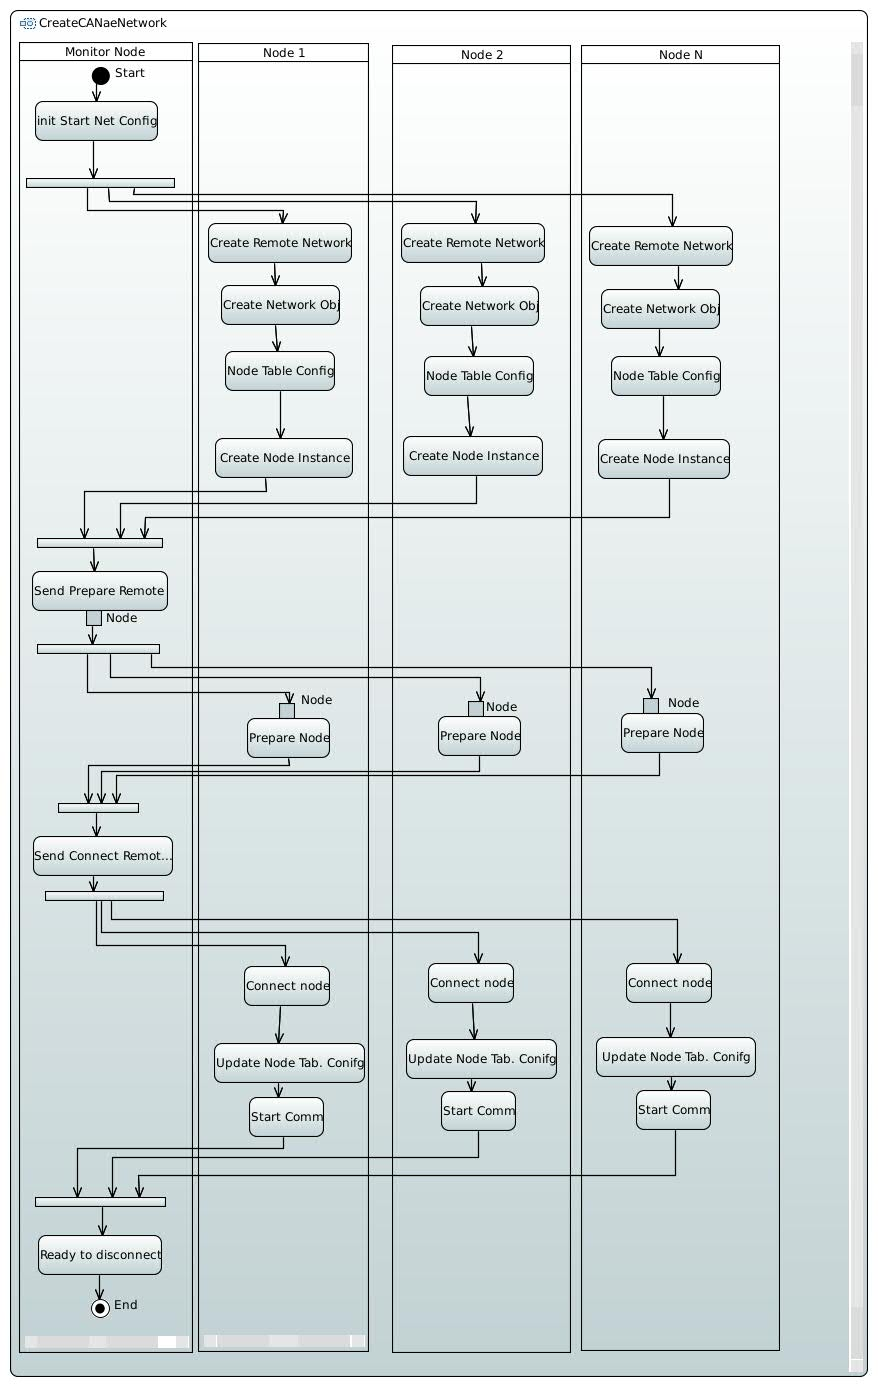
\includegraphics[scale=0.4]{images/Capitulo5/NodeMonitor.JPG}
  \caption{Diagrama de actividades del inicio de nodos}
  \label{fig:NodeMonitor}
\end{figure}

Como segundo paso, el nodo monitor envía la señal de \textit{Prepare Remote Node}, la
cual es recibida por todos los nodos y se preparan internamente para comenzar a
comunicarse.

Por último,  el nodo nodo monitor envía la señal para que los nodos se conecten a
la red. Cada nodo se conecta, y actualiza su tabla de configuración del nodo. A partir
de este momento los nodos ya pueden comenzar a enviar mensajes y el nodo monitor ya
puede ser extraído de la red. 

Además, se modela el ``cómo'' se comporta la arquitectura al
momento de tratar de enviar un mensaje de uno nodo a otro nodo. Esto se puede
observar en la Figura \ref{fig:SendMessage}. En primer lugar el nodo emisor,
debe ``preparar'' el mensaje. Esto significa que debe empaquetarlo para,
cumplir tanto con los protocolos CANae, como así también con el procolo CAN.

Como segundo paso se debe consultar a la tabla de configuación del nodo para conocer
cuál es el camino óptimo para llegar a entregar el mensaje. Para ello se le aplica algún
algoritmo de ruteo.

Por último, se envía el mensaje através del microcontrolador CAN. Este es recibido por el nodo
destino y luego es procesado. Esto puede observarse, con mayor detalle en el
apéndice \ref{Appendix:A}. 

\begin{figure}[h!]
 \centering
 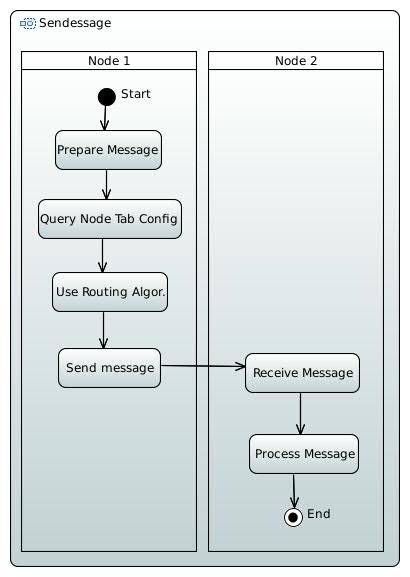
\includegraphics[scale=0.4]{images/Capitulo5/SendMessage.JPG}
  \caption{Diagrama de actividades del inicio de nodos}
  \label{fig:SendMessage}
\end{figure}


\chapter{Análisis y resultados}
\section{Introdución}
Si llego a implementar algo (que no creo a esta altura) colocar aquí el código y los resultados.


\chapter{Conclusión}
%\input

%\chapter{Área de estudio}
\label{chap:areadeestudio}




El área de las parcelas experimentales del \ac{cett} se encuentra ubicada en la provincia de Córdoba, al pié de las denominadas Sierras Chicas. Las coordenadas centrales del área de estudio son las siguientes: 31\textdegree31'15.08''S - 64\textdegree27'16.32''O (Fig. \ref{Fig:area_cett}). 

\imagen{0.5}{imagenes/AreaDeEstudio/Ubicacion.jpg}{Ubicación del área de estudio}{Fig:area_cett}

%\section*{Datos}
\label{sec:datos}
%\section*{Metodología}
\label{sec:metodologia}
%\chapter{Resultados}
\label{chap:resultados}




%\chapter{Discusión y lineamientos futuros}
\label{chap:discusion}

% ----------------------------------------------------------------------------------------------

\newpage
\nocite{*}
\bibliography{biblio.bib}
%\bibliographystyle{apalike}
\bibliographystyle{plainnatesp.bst}
\addcontentsline{toc}{chapter}{Bibliograf\'ia}

%------------------------------------------------------------------------------
% EN CASO DE TENER APÉNDICES, DESCOMENTAR A CONTINUACIÓN
\appendix
\chapter{Protocolo de comunicación: CANae 0.1 Alpha Version}\label{Appendix:A}
% introducción
\section{Introducción}
En este apéndice se explica el diseño de la versión Alpha del protocolo CANae. Este protocolo se basa en el la capa de aplicación del protocolo CAN y CANopen. El nombre CANae proviende de la unión de CAN y CONAE. 

\subsection{Revisiones}
\begin{table}[H]
  \centering
  \caption{Revisiones de CANae}
  \label{table:revisiones_canae}
  \begin{tabular}{|p{1cm}|p{2cm}|p{2cm}|p{5cm}|}
  \hline
  \multicolumn{1}{|c|}{\textbf{Ver.}} & \multicolumn{1}{c|}{\textbf{Who.}} & \multicolumn{1}{c|}{\textbf{When}} & \multicolumn{1}{c|}{\textbf{What}} \\ \hline \hline
 $0.1$ Alpha & Emmanuel Arias & 25/06/2017 & Initial Version \\ \hline
  \end{tabular}
\end{table}
\newpage


% Capa de aplicación
\section{Capa de aplicación}
La capa de aplicación de CANae está dividida entre la denominada \textit{CANae Application Layer} y la \textit{CANae High Application Layer} Figura\ref{fig:CANAE}. La funcionalidad que brinda la capa de aplicación está dividad en diferentes elementos de servicios dentro del a capa de aplicación. Un elemento de servicios brinda un determinado servicio.

\begin{figure}[h!]
 \centering
 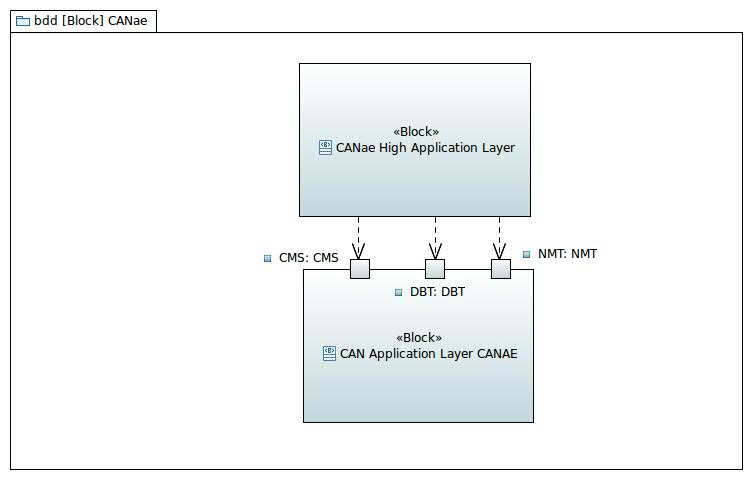
\includegraphics[scale=0.5]{images/Secciones/AppendixA/CANAE.jpg}
  \caption{Estructura de la capa de aplicación de CANae en alto nivel}
\label{fig:CANAE}
\end{figure}

Una capa de aplicación tiene las siguientes 4 funciones primitivas:
\begin{itemize}
\item Request: Una aplicación emite una petición a la capa de aplicación para solicitar un servicio.
  
\item Indication: Emitido por la capa de aplicación con destino una aplicación, para reportar de algún eveno interno detectado por la capa de aplicación, o indicar que un servicio fue solicitado.

\item Response: Emitido por la aplicación con destino la capa de aplicación para responder a una Indication previa.

\item Confirm: Emitido por la capa de aplicación para reportar el resultado de una peteción previa. 
\end{itemize}

\section{Tipos de servicios de la capa de aplicación}
Un tipo de servicio define las primitivas que intercambian las aplicaciones de usuario y los diferentes elementos de servicio que se encuentran dentro de la capa de aplicación. Los tipos de servicios posibles en CANae son los siguientes:
\begin{itemize}
\item Local serivice: Solo envuelve un elemento de servicio local. 

\item Confirmed service: Implica que uno o más elementos de servicio pares. La aplicación de usuario emite un request a su local service element. Este se transmite a sus elementos de servicios pares, la cual es enviada a la aplicación como una indicación. La otra aplicación emite un response que se transmite a la aplicación originante para confirmar la recepción del request. 

\item Provide initiated service: Implica solo el elemento de servicio local. El elemento de servicio detecta un evento no solicitado por la aplicación y emite una Indication. 
  
\end{itemize}

\section{CANae Application Layer}
En CANae se divide la tradicional capa de aplicación del modelo OSI en dos capas. En esta sección se estudia la \textit{CANae Application Layer}. Esta capa está conformada por 3 elementos de servicio:
\begin{itemize}
\item CAN based Message Specification (CMS): ofrece un ambiente orientado a objecto para diseñar aplicaciones de usuario. Esta entidad ofrece variables y eventos, y específica como un módulo pude acceder a las interfaces de CAN.
\item Network Managment (NMT): ofrece un ambiente orientado a objetos para permitir que un módulo (el NMT Master) se ocupe de la inicialización y posibles fallas  de otros módulos (NMT Slaves).
\item Distributor: ofrece el servicio para distribuir dinámicamente el identificador de para los diferentes nodos. 
\end{itemize}

Estos están basados en la capa de aplicación de CAN para la industria (CAN in Automation [CiA] International Users and Manufacturers Group e.V. CAN Application Layer for Industrial Applications). Estos elementos de servicios determinan el 'qué' puede hacer la capa. Estos son representados como interfaces(Figura \ref{fig:CANAE_APP_LAYER}).

\begin{figure}[h!]
 \centering
 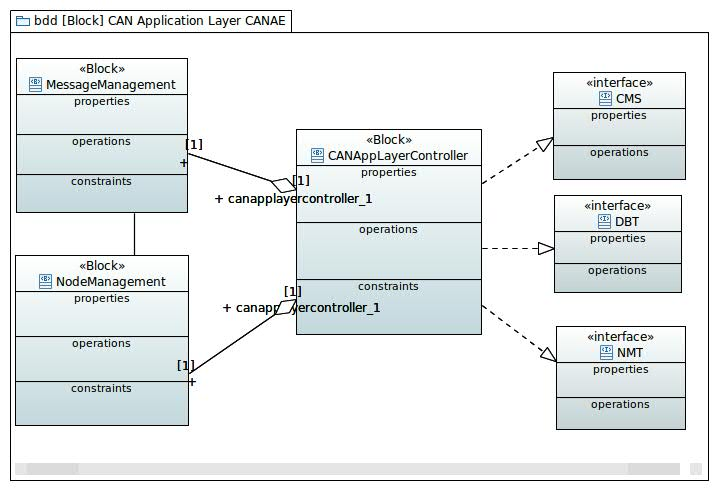
\includegraphics[scale=0.5]{images/Secciones/AppendixA/CAN_Application_Layer_CANAE.jpg}
  \caption{CANae Application Layer}
\label{fig:CANAE_APP_LAYER}
\end{figure}

Dentro de esta capa existen dos entidades importantes:
\begin{itemize}
\item Gestor de mensajes: este se encarga de gestionar los mensajes que son enviados y recibidos desde la red. Esta entidad debe ser capaz de determinar si el mensajes contiene datos o eventos. Trabaja en conjunto con el CMS.
  
\item Gestor de nodo: esta entidad se encarga de llevar el control de los nodos existenten en la red. En este nodo se encuentra la tabla de ruteo primario y secundario necesarios para la correcta comunicación.
  
\end{itemize}



% CMS
\section{CMS}
CMS ofrece un ambiente orientado a objeto para diseñar aplicaciones de usuario. CMS ofrece a la aplicación la posibilidad de modelar su comportamiento en la forma de objeto. Este elemento de servicio ofrece variables, eventos que se utilizan para diseñar y especificar como la funcionalidad de un módulo puede acceder a las interfaces CAN.

El servicio asume que no hay fallas provenientes de la capa de enlace de datos y la capa física de la red CAN. Las fallas, si ocurren, son resueltas por el NMSE (Network Management Service Element).

\subsection{Prioridades de los objetos}
La arbitración del protocolo CAN se realiza teniendo en cuenta la prioridad de los identificadores de los frames que se envía. La arbitración es no destructiva, debido a la necesidad de de tener un procesamiento de mensajes de tiempo real. La prioridad se determina teniendo en cuenta cada uno de los bits. El indentificador de los objetos y eventos de CMS está compuesto por 8 bits más 3 bits que los diferenciará entre objetos y eventos. Los eventos tiene mayor prioridad.

\begin{tabular}{lll}
    000 & (ID) & Tipo de evento \\
    111 & (ID) & Prioridad objeto \\
\end{tabular}

La prioridad de los objetos es un UInteger de 1 byte. La prioridad más baja es 0 y la prioridad más alta de 1. Por lo tanto la prioridad va desde 00000000b (mayor prioridad) hasta 11111111b (menor prioridad).

\subsection{Objeto CMS}
Un objeto CMS define una estructura de dato que se debe respetar para poder enviar información (variables) a través de la red. El objeto está compuesto por los siguientes campos:
\begin{itemize}
   \item Name: string de 6 caracteres (6 bytes)
   \item User\_type: {client, server} (1 bit)
   \item Priority: UInteger (1 bytes)
   \item Datatype: UInteger identificador del tipo de datos (1 byte)
   \item Data: Indefinido.
\end{itemize}

\begin{figure}[h!]
 \centering
 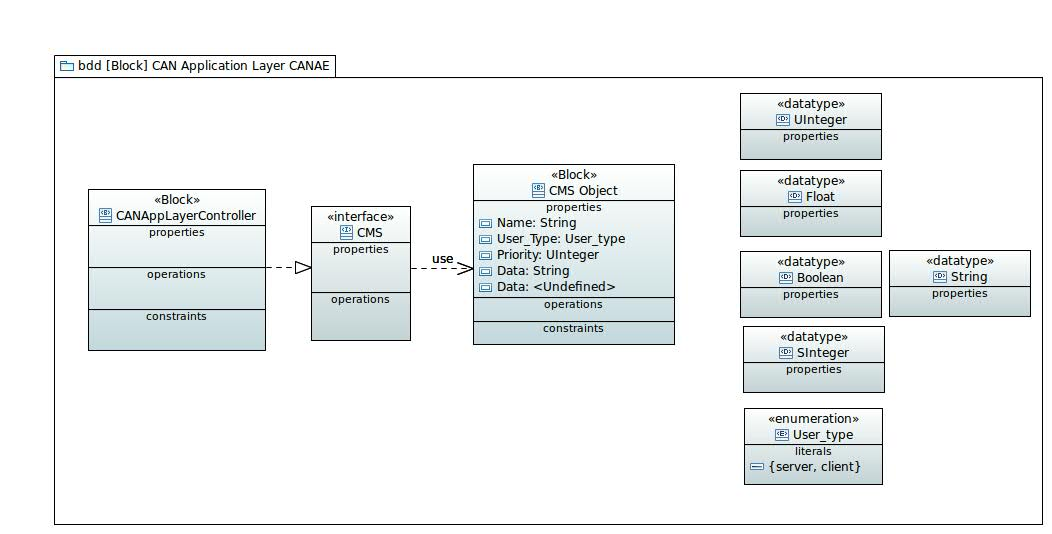
\includegraphics[scale=0.4]{images/Secciones/AppendixA/CMSObject.JPG}
  \caption{Definición del Objeto CMS}
\label{fig:CMSObject}
\end{figure} 

\subsection{Servicios de CMS}
Con respecto a las variables de CMS existen una serie de servicios brindados por CMS, que pueden ser tanto \textit{local services} como \textit{remote services}. Su clasificación depende de si se está accediendo a variables almacenadas dentro del nodo, o bien se está intentando acceder (escribir o leer) una variable remota. Un evento está definido de la siguiente manera:

\begin{itemize}
   \item Name: string de 6 caracteres (6 bytes)
   \item User\_type: {client, server} (1 bit)
   \item Priority: UInteger (1 bytes)
   \item Event\_Type: UInteger identificador del tipo de datos (1 byte)
   \item Data: Indefinido.
\end{itemize}


\subsubsection{Servicios locales}
\begin{itemize}
  
\item Boolean define\_variable(String name, DataType data\_type)
  \begin{itemize}
  \item \textbf{String name}: Nombre de la variable.
    \item \textbf{DataType data\_type}: Tipo de dato de la variable. 
  \end{itemize}
  
\item Boolean set\_variable(String name, UInteger destination, Data data, UInteger priority)
  \begin{itemize}
    \item \textbf{String name}: Nombre de la variable.  
    \item \textbf{UInteger destination}: Direción del destinatario. Esta dirección debe ser provista por el NMT.
    \item \textbf{Data data}: Datos a enviar.
    \item \textbf{UInteger priority}: Prioridad de la variable.
  \end{itemize}
  
\item Boolean update\_variable(String name, data data)
  \begin{itemize}
    \item \textbf{String name}: Nombre de la variable
    \item \textbf{Data data}: Datos a enviar    
  \end{itemize}
 
\end{itemize}
\subsubsection{Servicios remotos}
\begin{itemize}
\item Boolean write\_variable(String name, Data data)
  \begin{itemize}
    \item \textbf{String name}: Nombre de la variable a escribir
    \item \textbf{Data data}: Dato a escribir
  \end{itemize}
\item Data read\_variable(String name)
  \begin{itemize}
    \item \textbf{String name}: Nombre de la variable a leer
  \end{itemize}
\end{itemize}

\subsection{Eventos}
Los eventos se utilizan para modelar comportamientos asíncronos, tales como temperatura excedida en un tiempo determinado. La ocurrencia de los eventos es detectada por el nodo, que en ese momento actuará como server y se notifica a todos los clientes.
\begin{comment}
\begin{figure}[h!]
 \centering
 \includegraphics[scale=0.4]{images/Secciones/AppendixA/CMSEvent.JPG}
  \caption{Definición del Objeto CMS}
\label{fig:CMSEvent}
\end{figure} 
\end{comment}
Los servicios al igual que las variables se dividen los eventos brindados por servicio local o servicio remoto. Los servicios se describen a continuación.

\subsubsection{Servicios locales}
\begin{itemize}
\item define\_event(String name, UInteger priority, UInteger event\_type)
  \begin{itemize}
  \item \textbf{String name}: Nombre del evento
  \item \textbf{UInteger priority}: Prioridad del evento
  \item \textbf{UInteger event\_type}: Tipo de evento según tabla \ref{table:prioridad_eventos}
  \end{itemize}

\end{itemize}

\subsubsection{Setvicios remotos}

\begin{itemize}
\item Event notify\_event()
\item Boolean store\_event(String name)
  \begin{itemize}
    \item \textbf{String name}: Nombre de evento a almacenar
  \end{itemize}
  
\item Event read\_event(String name)
  \begin{itemize}
    \item \textbf{String name}: Nombre de la variable a leer
  \end{itemize}
\end{itemize}

\subsubsection{Prioridad de eventos}
La prioridad de los eventos se define como una tabla que se define al momento de implementar el protocolo. Al desarrollar la tabla de prioridades se debe cuidar la relevancia de los eventos. La prioridad más baja es 0. El tamaño de la prioridad del evento es de 1 byte. Por lo tanto la prioridad va desde 00000000b (mayor prioridad) hasta 11111111b (menor prioridad).

\begin{table}[h!]
  \centering
  \caption{Prioridad eventos}
  \label{table:prioridad_eventos}
  \begin{tabular}{|l|l|l}
    \cline{1-2}
    00000000 & Nombre evento & Mayor prioridad \\\cline{1-2}
    00000001 & Nombre evento & \\\cline{1-2}
    00000010 & Nombre eevnto & \\\cline{1-2}
    ... & ... & ... \\\cline{1-2}
    11111111 & Nombre evento & Menor prioridad \\\cline{1-2}
  \end{tabular}    
\end{table}

Esta tabla de prioridad de eventos, debe ir acompañada de un diccionario de eventos, donde se almacena los datos relevantes al evento. En esta se hace una descripción del evento. Sirve de guía para la implementación y desarrollo de aplicaciones que identifican eventos.

El diccionario debería incluir los siguientes campos:
\begin{itemize}
\item Nombre del evento
\item Descripción del evento
\item Prioridad
\item Umbral límite inferior (En el caso de que existiera)
\item Umbral límite superior (En el caso de que existiera)
\end{itemize}




% NMT
\section{NMT}\label{Appendix:NMT}
Esta es una entidad de la capa de aplicación que permite el correcto
funcionamiento de la red. Esta entidad tiene los servicios necesarios para que
cada nodo tenga un conocimiento de todos los nodos conectados en la red. Esto
permite el armado de una tabla de nodos, que es mantenida en todo los
nodos. Esta entidad exige la existencia de un nodo monitor, que es el encargado
de monitorear y configurar la red. Luego, una vez en funcionamiento este nodo
monitor no será vital para la red. En el NMT se deben implementar los
algoritmos de ruteo. El entorno NMT se puede observar en la Figura
\ref{fig:NMT}. Se puede observar también el diagrama de bloques internos en
la Figura \ref{fig:NMTInterno}

\begin{figure}[h!]
 \centering
 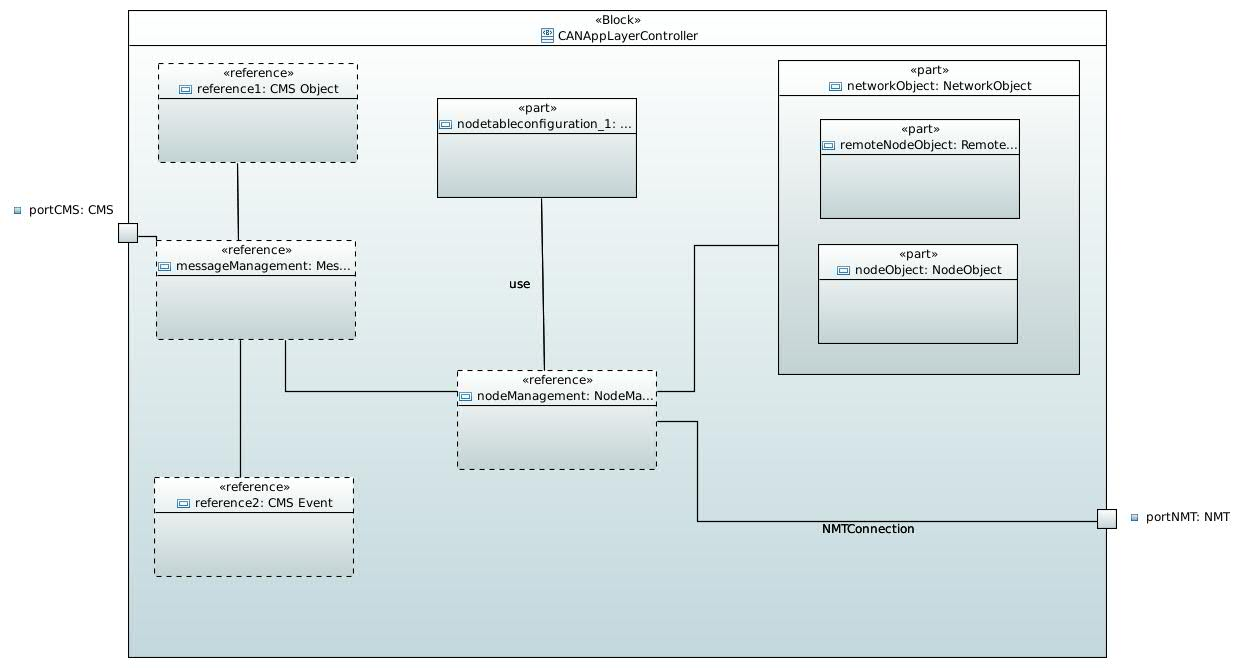
\includegraphics[scale=0.4]{images/Secciones/AppendixA/CANae_Application_Layer_Controller.JPG}
  \caption{Definición de la entidad NMT (bloques internos)}
\label{fig:NMTInterno}
\end{figure} 

\begin{figure}[h!]
 \centering
 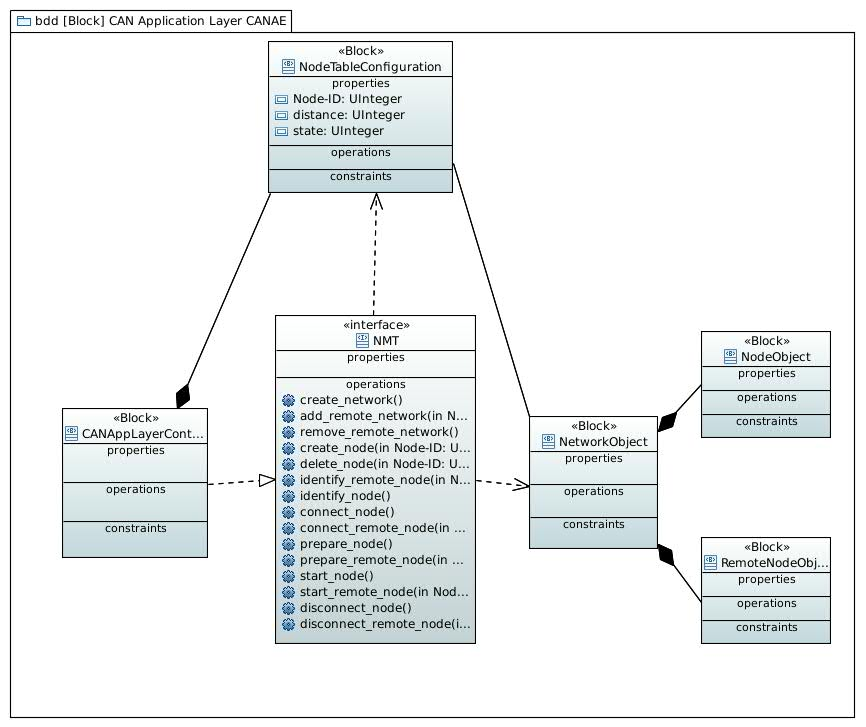
\includegraphics[scale=0.4]{images/Secciones/AppendixA/NMT.JPG}
  \caption{Definición de la entidad NMT}
\label{fig:NMT}
\end{figure} 

Por medio de este servicio es posible conocer el estado de la red CAN. Los
mensajes de NMT CAN son envíados con máxima prioridad. 
\subsection{Objectos NMT}
El Network Management utiliza tres objetos diferentes para modelar una red CAN.
\begin{itemize}
 \item \textbf{Network Object}: Representa todos los módulos conectados en la
  red CAN. El objeto de red existe en todos los nodos.
 \item \textbf{Remote Node Object}: Cada nodo conectado a la red CAN tiene
   representado todos los demás nodos.    
 \item \textbf{Node Object}: Cada nodo que es gestionado por el servicio NMT
   está representado por un node object. Este objeto se encuentra modelado en
   cada uno de los nodos.    
 \end{itemize}
Cada nodo y su objeto (remoto y local) es unívocamente identificado en la red
por su NMT Address. Esta dirección no se puede cambiar. Esto significa que por
cada nodo existe un objeto nodo y un objeto nodo remoto con el mismo NMT
Address, replicada en todos los nodos de la red. 

\subsection{Servicios NMT}
La entidad NMT ofrece los siguientes servicios:
\subsubsection{Module Control Service}
EL NMT monitor incializa los nodos NMT que forman parte de la red CAN
distribuida, a través de este servicio se asegura que todos los nodos se
encuentran configurados y funcionando correctamente.
\subsubsection{Error Control Services}
Através de este servicio, el NMT detecta fallas en la red CAN, ya sea fallas
producidas en la capa de enlace de datos (fallas locales) y/o fallas
producidos en otros nodos.
\subsubsection{Configuration Control Services}
Através de este servicio se realiza la configuarción de la red.

\subsubsection{Servicios a implementar}\label{subsubsection_servicios_implementar}
La funciones típicas que se deben implementar en el NMT son los siguientes:
\begin{itemize}
\item Boolean create\_network()
\item Boolean create\_remote\_network() 
\item Boolean remove\_remote\_network()
\item Boolean create\_node(UInteger Node-ID, UInteger address, String description)
  \begin{itemize}
  \item \textbf{UInteger Node-ID}: ID del nodo a crear.
  \item \textbf{UInteger address}: Dirección del nodo creado. UInteger entre [0,255]
  \item \textbf{String description}: Descripción del nodo.
  \end{itemize}
\item Boolean delete\_node(UInteger Node-ID)
  \begin{itemize}
   \item \textbf{UInteger Node-ID}: Dirección del nodo a eliminar. UInteger entre [0,255]
  \end{itemize}
    
\item UInteger identify\_remote\_node(UInteger Node-ID)
  \begin{itemize}
  \item \textbf{UInteger Node-ID}: Dirección del nodo a identificar
  \end{itemize}

\item UInteger identify\_node()
  
\item Boolean connect\_node()
  
\item Boolean connect\_remote\_node(UInteger Node-ID)
  \begin{itemize}
    \item \textbf{UInteger Node-ID}: ID del nodo remoto a conectar.
  \end{itemize}

\item Boolean prepare\_node()
\item Boolean prepare\_remote\_node(UInteger Node-ID)
  \begin{itemize}
   \item \textbf{UInteger Node-ID}: ID del nodo a pasar a modo preparado
  \end{itemize}
\item Boolean start\_node()
\item Boolean start\_remote\_node(UInteger Node-ID)
  \begin{itemize}
    \item \textbf{UIntenger Node-ID}: ID del nodo que comenzará a participar en la red.
   \end{itemize}
\item Boolean disconnect\_node()
\item Boolean disconnect\_remote\_node(UInteger Node-ID)
  \begin{itemize}
    \item \textbf{UInteger Node-ID}: ID del nodo a desconectar.
  \end{itemize}
\end{itemize}

\subsection{Protocolos NMT}
\subsubsection{Crear red CANae}
Para conectar correctamente la red CANae se debe respetar el protocolo NMT para
crear la red. En primer lugar el nodo monitor debe enviar el mensaje
\textit{create\_remote\_network()} para avisar a todos los nodos que deben crear
sus propias instancias de \textit{NetworkObject} a través de
\textit{create\_network()}. Automáticamente, los nodos deben crear una propia
instancia del nodo mediante \textit{create\_node()}. Luego, el nodo monitor
envía el mensaje de \textit{prepare\_remote\_node()} para prepara todos los
nodos a conectarse a la red CANae. Paso siguiente, el nodo monitor envía la señal de
\textit{connect\_remote\_node(UInteger Node-ID)} con la dirección de todos los
nodos que figuran en \textit{NodeTableConfiguration} preprogramada.
Así, cada nodo, correctamente preparado, se conecta a la red a través de
\textit{connect\_node()}.

Este protocolo puede ser observado en la Figura \ref{fig:ProtocolNMTConnectNet}
\begin{figure}[h!]
 \centering
 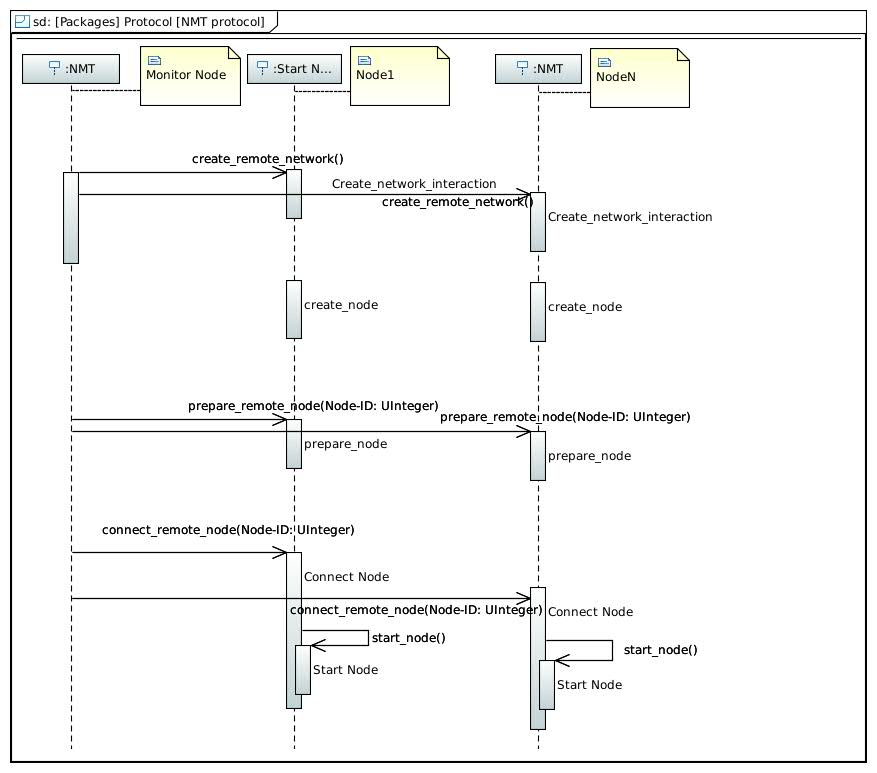
\includegraphics[scale=0.4]{images/Secciones/AppendixA/Protocol_NMT.JPG}
  \caption{Protocolo NMT}
  \label{fig:ProtocolNMTConnectNet}
\end{figure} 

\subsubsection{Crear Red}\label{NMT:crear_red}
Para lograr la correcta conexión de los nodos a la red, estos deben
configurarse. Cuando se alimenta la red, los nodos deben iniciar en estado de
\textit{escucha} esperando la orden del nodo monitor de crear la red mediante
\textit{create\_remote\_network()}. Esta se envía en broadcast a todos los nodos
conectados. Cuando el controlador de la capa de aplicación recibe el mensaje
através del servicio NMT, este manda un mensaje al gestor del nodo interno, el
cual crea la \textit{tabla de configuración del nodo} y la  actualiza con la
información necesaria.

\begin{figure}[h!]
 \centering
 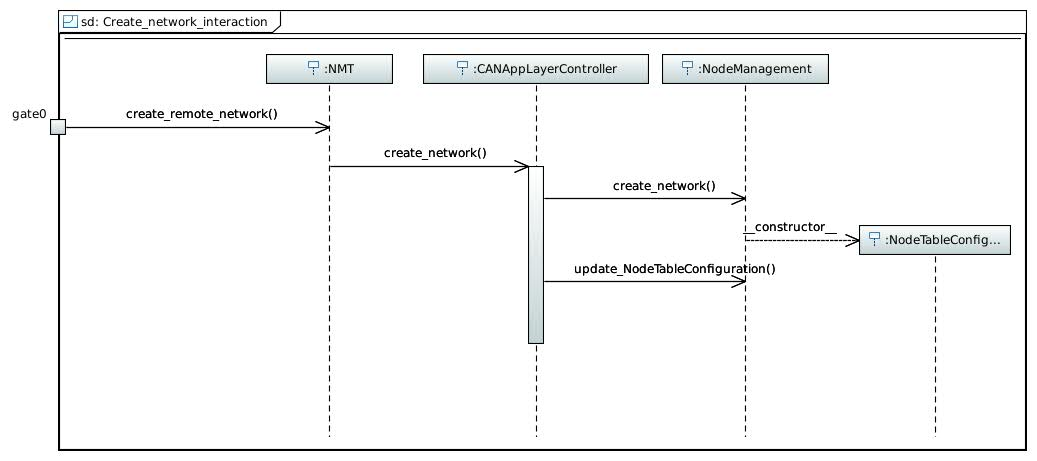
\includegraphics[scale=0.4]{images/Secciones/AppendixA/Create_Network.JPG}
  \caption{Crear Red}
  \label{fig:CreateNetwork}
\end{figure} 

\subsubsection{Crear Objecto Red, Objeto Nodo y Objeto Nodo Remoto}
Antes de comenzar a funcionar la red, cada nodo debe crear un objeto de red
exigidos por el protocolo NMT. Una vez que el proceso Crear Red termina,
el Gestor de la capa de Aplicación envía un mensaje \textit{create\_node()}
al Gestor del Nodo. El Gestor de Nodo crea un \textit{Network Object}. Este a su
vez crea un \textit{Node Object} y un \textit{Remote Node Object}. Estos objetos
pertenecen a la entidad NMT (Figura \ref{fig:CreateNode}).

\begin{figure}[h!]
 \centering
 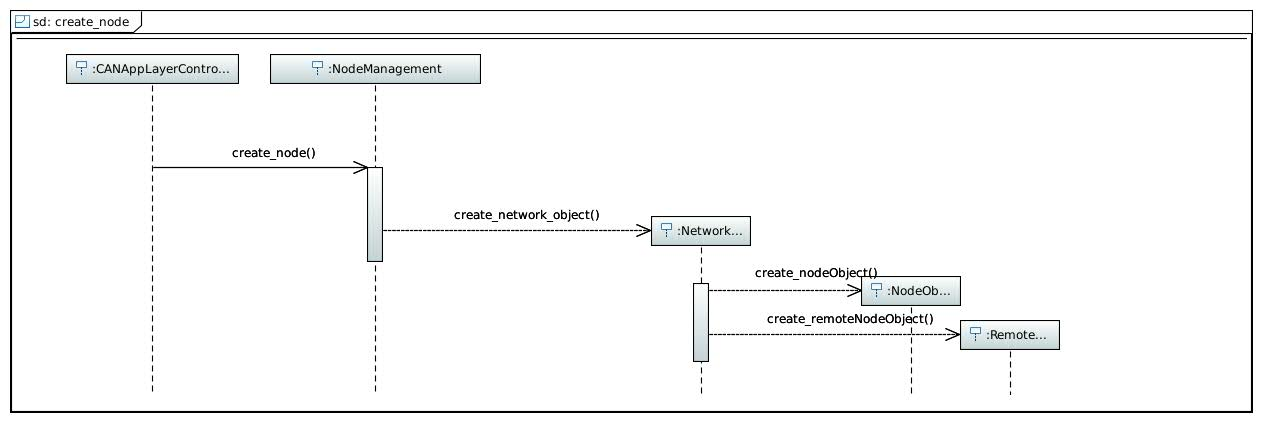
\includegraphics[scale=0.4]{images/Secciones/AppendixA/create_node.JPG}
  \caption{Crear Objecto Red, Objeto Nodo y Objeto Nodo Remoto}
  \label{fig:CreateNode}
\end{figure}

\subsubsection{Preparar nodos para conexión}
Para lograr la conexión de los nodos a la red CAN, es necesario que el nodo
monitor envíe la señal \textit{prepare\_remote\_node(UInteger Nodo-ID)} a
cada uno de los nodos conectados a la red siguiendo la propia tabla de
configuración de nodos preprogramada. Cada nodo recibe la señal procesa aquella
que le pertence, y comienza a preparar el nodo para lograr la correcta conexión.
Para ello debe actualizar su propia tabla de configuración de nodos, como así
también actualizar su \textit{Objeto Red} (Figura \ref{fig:PrepareNode}).

\begin{figure}[h!]
 \centering
 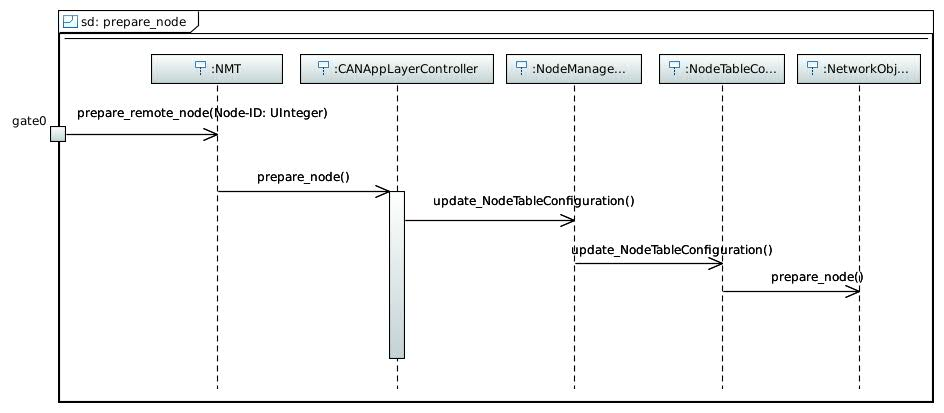
\includegraphics[scale=0.4]{images/Secciones/AppendixA/PrepareNode.JPG}
  \caption{Preparar nodo para la conexión a la red CAN}
  \label{fig:PrepareNode}
\end{figure}

\subsubsection{Conectar nodos en la red}
Para conectar los nodos a al red se tiene que modificar al información de la
\textit{Node Table Configuration} y en el \textit{Objeto de Red}. Una vez
realizado esto se puede comenzar con la comunicación de los nodos
(Figura \ref{fig:ConnectNode}).

\begin{figure}[h!]
 \centering
 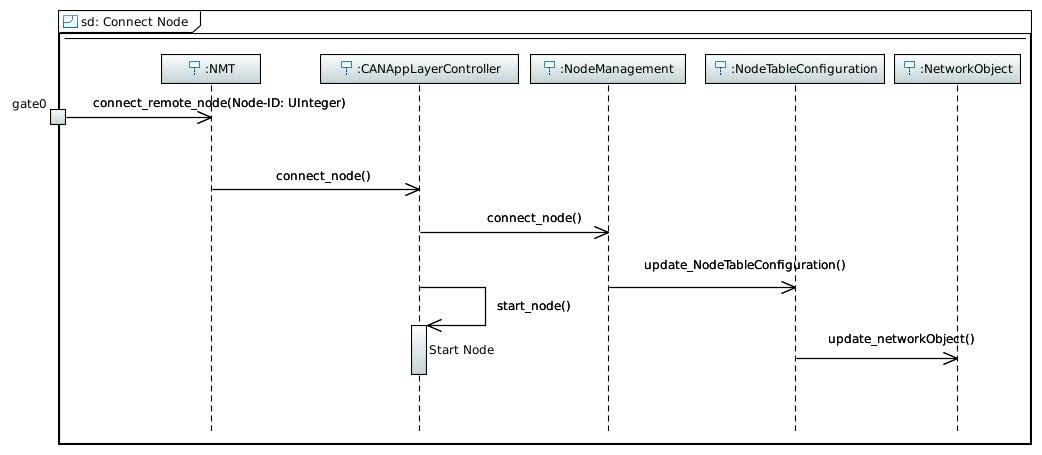
\includegraphics[scale=0.4]{images/Secciones/AppendixA/connect_node.JPG}
  \caption{Conectar el nodo a la red CAN}
  \label{fig:ConnectNode}
\end{figure}

\subsubsection{Comenzar la comunicación}
Para que el nodo pueda comenzar a comunicar debe encontrarse en un estado
\textit{Start}. Esto representa una actualización de la
\textit{Node Table Configuration} y del \textit{Objeto de Red}
(Figura \ref{fig:StartNode}). 

\begin{figure}[h!]
 \centering
 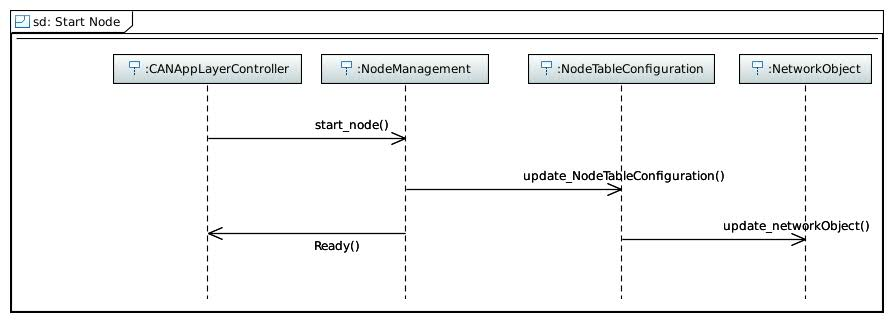
\includegraphics[scale=0.4]{images/Secciones/AppendixA/Start_Node.JPG}
  \caption{Comenzar la comunicación de nodos}
  \label{fig:StartNode}
\end{figure}







































































































































































































% DBT
\section{DBT}\label{Appendix:DBT}
La principal complicación del desarrollo de una red distribuída basada en el BUS
CAN, es que puedan comunicarse correctamente entre sí, cómo se deben asignar
los identificadores (Node-ID) correctamente a cada uno de los nodos y cómo se
asignan los tiempos de inhibición. Los Node-ID y los tiempos de inhibición se
deben distribuir entre los nodos de tal manera de asegurar que:
\begin{itemize}
\item Se preveean los conflictos entre nodos. Por ejemplo, diferentes funciones
  que usan el mismo identificador.
\item Se preveean la falta de coincidencia. Por ejemplo, que existan diferentes
  indentificadores para el mismo nodo.
\item ofrecer el control integrado para un comportamiento dinámico del
  sistema.  
\end{itemize}

El protocolo CAN (CAN Application Layer for Industrial Applications
CiA/DS204-1) dispone la existencia de 3 métodos para distribuir identificadores
y tiempo de inhibición a un módulo.

\begin{itemize}
\item \textbf{Distribución estándar}: en este método los identificadores y
  tiempos de inhibición son estandarizados por el módulo proveedor (nodo
  monitor. Una distribución estándar require la estandarización de todas las
  funciones y su correspondiente identificador.
\item \textbf{Distibución estática}: En este método los identificadores y los
  tiempos de inhibición son fijos. Todos los identificadores y los tiempos de
  inhibición son fijados en el momento del desarrollo.
\item \textbf{Distribución dinámica}: En este método los identificadores y los
  tiempos de inhibición son distribuidos vía red CAN a través del servicio
  estándar y un protocolo definido.  
\end{itemize}

En esta instancia de trabajo, para el desarrollo del protocolo CANae, se utilizó
el \textit{método de distribución estática}. Esto exige que los nodos ya cuenten
con un identificador y tiempos de inhibición por defecto. Esto se asigna en el
momento del desarrollo del diseño e ingeniería de la arquitectura de aviónica.
Esto reduce considerablemente la complejidad de la entidad DBT. Si bien
originalmente, el DBT es un elemento de servicio de la capa de aplicación CAN
que ofrece una distribución dinámica de identificadores y tiempos de inhibición,
en CANae es utilizado para asegurar la correcta comunicación y consistencia de
los nodos y la red en su conjunto.

La arquitectura del DBT se puede observar en la Figura \ref{fig:DBT}

\begin{figure}[h!]
 \centering
 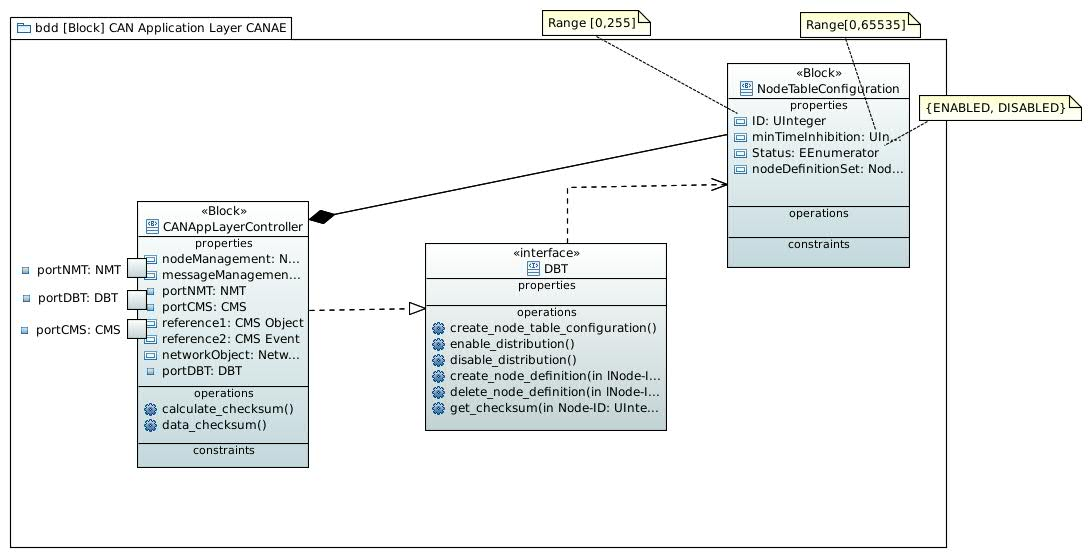
\includegraphics[scale=0.4]{images/Secciones/AppendixA/DBT.JPG}
  \caption{Arquitectura de la entidad DBT}
\label{fig:DBT}
\end{figure} 

\subsection{Objetos y servicios de DBT}
El DBT de CANae utiliza 2 objetos para modelar su funcionamiento:
\begin{itemize}
\item \textbf{Node-ID Database (NodeTableConfiguration)}: Esta tabla contiene la
  definición de todos los nodos conectados a la red. Esta tabla está compuesta
  por Node-ID Definitions
\item \textbf{Node-ID Definition}: define todos los atributos de un Node-ID.
  Contiene una definición de usuario creado por el usuario.
\end{itemize}

El DBT de CANae ofrece las siguientes categorias de servicio:
\begin{itemize}
\item \textbf{Distribution Control Services}: esta es tarea del nodo monitor de
  enviar el identificador y los tiempos de inhibición a todos los nodos
  conectados a la red. Los datos que son enviados por el nodo monitor son
  corroborados por los nodos, comprobando que el ID enviado coincida con su
  propio Node-ID.
\item \textbf{Consistency Control Services}: através de este servicio cada nodo
  puede detectar inconsistencia en el \textit{NodeTableConfiguration} e inconsistencia
  entre nodos.
\end{itemize}

\subsection{Descripción de los servicios DBT}
Los servicios se describen en forma de tabla que contiene los parámetros de
cada función que se define para ese servicio. Los parámetros determinan el tipo
de servicio.  Todos los servicios asumen que no ocurrieron ningún tipo de error
en la capa de física ni en la capa de enlace de datos.

\subsection{Objetos DBT}
Los objetos que utiliza la entidad DBT para modelar el servicio son los
siguientes:
\begin{itemize}
\item \textbf{Node Table Configuration (Node-ID Database)}
  \begin{itemize}
  \item \textbf{Atributos}
    \begin{itemize}
    \item \underline{Estado}: Uno de los valores {ENABLED, DISABLED}. Este
      atributo indica si el DBT Monitor es capaz de distribuir los Node-ID
      y tiempos de inhibición. En esta instancia de trabajo el valor del estado
      en el DBT del Nodo Monitor será DISABLED
      \item \underline{Node Definition Set} set de todas las definiciones. 
    \end{itemize}
  \end{itemize}

\item \textbf{Node-ID Defintion}:
  Las definiciones contiene los siguientes datos:
  \begin{itemize}
  \item \underline{ID}: Valor en el rango de [0,255]
  \item \underline{Mínimo tiempo de inhibición}: en el rango [0,65535] indicando
    el valor mínimo en unidades de 100$\mu$sec para el tiempo de inhibición.
  \end{itemize}
  
\end{itemize}

\subsection{Servicios DBT}\label{subsection:servicios_dbt}
\subsubsection{Distribution Control Services}
\begin{itemize}
  \item create\_node\_table\_configuration()
  \item enable\_distribution()
  \item disable\_distribution()
  \item create\_node\_definition(UInteger lNode-ID, UInteger hNode-ID, UInteger minInhibitTime)
    \begin{itemize}
    \item \textbf{UInteger lNode-ID}: Límite inferior del rango de IDs.
    \item \textbf{UInteger hNode-ID}: Límite superior del rango de IDs.
    \item \textbf{UInteger minInhibitTime}: Tiempo mínimo de inhibición de cada
      nodo.
    \end{itemize}
  \item delete\_node\_definition(UInteger lNode-ID, UInteger hNode-ID)
\end{itemize}

\subsubsection{Consistency Control Service}

\begin{itemize}
\item get\_checksum(UInteger Node-ID, Float checksum)
  \begin{itemize}
      \item \textbf{UInteger Node-ID}: ID del nodo que desea controlar la
    consistencia.
      \item \textbf{UInteger checksum}: checksum de la DBT Definition.
  \end{itemize}
\end{itemize}


\subsection{Protocolos DBT}
\subsubsection{Crear NodeTableConfiguration}
En la tabla de configuración del nodo juega un papel similar al que lo haría el
Node-ID DATABASE del estándar CAN. La principal diferencia, es que esta tabla
se encuentra presente en todos los nodo y no en el ``Master'', ya que este
protocolo está pensado para ser utilizado en redes distribuidas, donde no
existe un nodo central o master.

El nodo monitor envía la señal a los nodos de crear la tabla de configuración
del nodo através de \textit{create\_node\_table\_configuration()}. Este es
recibido através de la interfaz DBT del nodo, y crea el objeto
\textit{NodeTableConfiguration}. Esto se observa en la Figura
\ref{fig:createNodeTableConfiguration}.

\begin{figure}[h!]
 \centering
 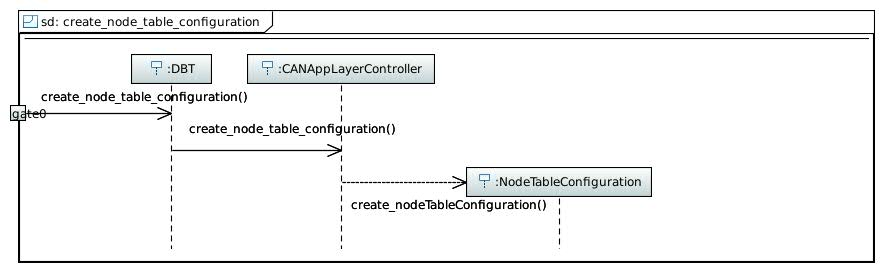
\includegraphics[scale=0.4]{images/Secciones/AppendixA/create_node_table_configuration.JPG}
  \caption{Protocolo create\_node\_table\_configuration}
\label{fig:createNodeTableConfiguration}
\end{figure} 

\subsubsection{Habilitar distribución}
La distribución de Node-ID es utilizada cuando se usa el método de
asignación dinámica. En esta versión del protocolo la distribución del ID se
encuentra desactivada. En la Figura \ref{fig:enable_distribution} se puede
observar el protocolo.

\begin{figure}[h!]
 \centering
 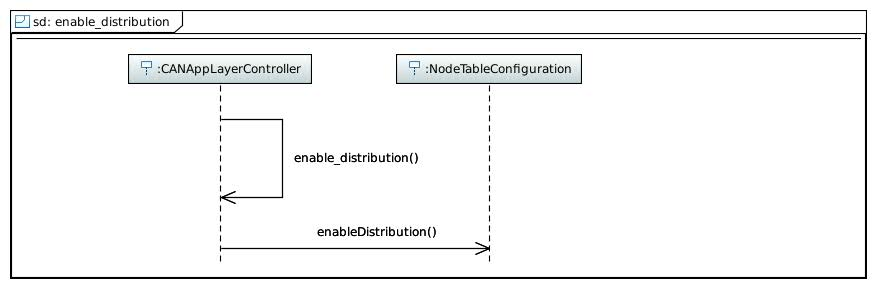
\includegraphics[scale=0.4]{images/Secciones/AppendixA/enableDistribution.JPG}
  \caption{Protocolo enable\_distribution}
\label{fig:enable_distribution}
\end{figure}

\subsubsection{Deshabilitar distribución}
Esta opción se encuentra por defecto en esta versión del protocolo CANae. El ID
se distribuye estáticamente. Son preestablecidos durante el desarrollo. En la
Figura \ref{fig:disable_distribution}

\begin{figure}[h!]
 \centering
 \includegraphics[scale=0.4]{images/Secciones/AppendixA/disable_distribution.JPG}
  \caption{Protocolo disable\_distribution}
\label{fig:disable_distribution}
\end{figure}


\subsubsection{Crear definición del nodo}
El nodo monitor envía la señal para crear las definiciones del nodo. Para
ello es necesario que el nodo monitor envíe los rangos permitidos para la
definición de los nodos. Esto se define a través de las variables
\textit{lNode-ID} y \textit{hNode-ID}. En esta versión del protocolo estas
variables no son utilizadas ya que los Node-ID ya se encuentran definidas
estáticamente. También el nodo monitor envía el tiempo mínimo de inhibición
explicado anteriormente. El nodo monitor hace este proceso con todos los nodos
de la red a través del mensaje \textit{create\_node\_definition}. Este se lo
puede observar en la Figura \ref{fig:create_node_definition}.

\begin{figure}[h!]
 \centering
 \includegraphics[scale=0.4]{images/Secciones/AppendixA/create_node_definition.JPG}
  \caption{Protocolo create\_node\_definition}
\label{fig:create_node_definition}
\end{figure}


\subsubsection{Eliminar la definición del nodo}
Esta función es utilizada para eliminar la definción del nodo. Se lleva a cabo
para eliminar un nodo de la red. Se hace através de la función
\textit{delete\_node\_definition()}. Esta se la puede observar en la Figura
\ref{fig:delete_node_definition}

\begin{figure}[h!]
 \centering
 \includegraphics[scale=0.4]{images/Secciones/AppendixA/create_node_definition.JPG}
  \caption{Protocolo delete\_node\_definition}
\label{fig:delete_node_definition}
\end{figure}


\subsubsection{Checksum}
Para poder asegurar la integridad de los nodos conectados a la red, se puede
utilizar este mecanismo para comprobar de que la información, referente a
la definición de los nodos, se encuentra correctamente en todos los nodos. Para
ello, cada nodo lleva a cabo un checksum de su información y la envía por la
red. Como esta está basada en el Bus-CAN, el mensaje llega correctamente a todos
los nodos. Los nodos realizan sus comprobaciones y responden. Si la información
es correcta deben responder con un mensaje que contegan bits NO dominantes. En
el caso de que se produzca alguna diferencia en los checksum deberán responder
con bits dominantes. Cuando esto se produzca deberán llevarse a cabo medidas de
recuperación o reconfiguración de la red. Este protocolo se lo puede observar en
la Figura \ref{fig:get_checksum}

\begin{figure}[h!]
 \centering
 \includegraphics[scale=0.4]{images/Secciones/AppendixA/get_checksum.JPG}
  \caption{Protocolo get\_checksum}
\label{fig:get_checksum}
\end{figure}


% Management message
\section{Gestor de mensajes}
El \textbf{Message Management} se encarga de gestionar los mensajes que son
enviados y recibidos desde la red CAN. Esta entidad debe ser capaz de determinar
si el mensaje (enviado o recibido) contiene datos o eventos. El gestor de
mensajes tiene cuatro entidades:
\begin{itemize}
\item \textit{Receiver Manager}: es el encargado de recibir los mansajes de la
  capa inferior a traves de la interfaz NMT. Esta entidad recibe y despaquetiza
  los mensajes.
\item \textit{Prepared Message}: es el encargado de recibir los mensajes desde
  las capas superiores para ser enviado a la red.
\item \textit{Sorter Message}: es el encargado de clasificar los mensajes,
  ya sea aquellos que envía a la red CAN comos los que recibe de esta. Su
  principal función es verificar  el tipo de mensaje que está recibiendo o
  enviando (datos o eventos). Los eventos tiene mayor prioridad que los datos
  y deben atenderse con urgencia.
\item \textit{Buffer Message}: este sirve de buffer para almacenar mensajes
  tanto que se envían como lo que se reciben. Este buffer es utilizado por el
  \textit{Sorter Message}.
\end{itemize}

\todo[inline]{AGREGAR IMAGEN}
\begin{figure}[h!]
 \centering
 \includegraphics[scale=0.4]{images/Secciones/AppendixA/DBT.JPG}
  \caption{Arquitectura de la entidad DBT}
\label{fig:DBT}
\end{figure}


\subsection{Receiver Manager}
Esta entidad perteneciente al \textit{Message Management} se encarga de recibir
los mensajes de la capa inmediatamente inferior a través de la interfaz NMT (y
sus protocolos). Esta entidad recibe y despaquetiza los paquetes. Se supone que
los mensajes llegan sin ningún tipo de error.

Las principales funciones de esta entidad son las siguientes:
\begin{itemize}
\item receive\_message(Message message): esta es la operación que se debe llamar
  para recibir el mensaje proveniente de la capa inferior. 
  \begin{itemize}
  \item \textbf{Data message}: Es el mensaje que recibe de las capas inferiores
    de la red CAN.
  \end{itemize}
\end{itemize}

\subsection{Sorter Message}
Esta entidad es el encargado de clasificar los mensajes que provienen tanto del
\textit{Receiver Message} y \textit{Prepared Message}. Este clasifica los
mensajes recibidos o por enviar, de modo tal de conocer aquellos que sean
datos o eventos. Debe tenerse en cuenta que los eventos tiene mayor prioridad
que los datos, debido a que (en su mayoría) informan de algún problema a la red.

Las principales funciones con las que cuenta esta entidad son las siguiente:
\begin{itemize}
  \item Boolean extract\_type\_message(Data message): esta operación permite
  extraer el tipo de información que contiene el mensaje: datos o evento.
  \begin{itemize}
  \item \textbf{Data message}: es el mensaje que recibe de las capas inferiores
    de la red CAN.
  \item \textbf{Return Boolean}: retorna 1 se se trata de un evento, 0 si se
    trata de un dato.
  \end{itemize}

\item Boolean send\_message(Message message): esta función envía los mensajes
  a las capas inferiores a través del protocol NMT.
  \begin{itemize}
  \item \textbf{Message message}: es el mensaje formateado listo para enviar.
  \item \textbf{Return Boolean}: retorna 1 si la operación se llevó
    correctamente.
  \end{itemize}
\item Boolean send\_event(Message message): esta función envía el evento en
  forma de mensajes formateado. 
    \begin{itemize}
  \item \textbf{Message message}: es el mensaje formateado listo para enviar.
  \item \textbf{Return Boolean}: retorna 1 si la operación se llevó
    correctamente.
  \end{itemize}
\end{itemize}


\subsection{Buffer Messages}
Esta es la entidad que permite almacenar los mensajes que son recibidos y
enviados. Esta entidad debe controlar la integridad de los mensajes que se
encuentran almacenados. Además se encarga de escribir y leer los mensajes
almacenados en el buffer. El buffer es FIFO\footnote{First In First Out}.

Las principales funciones de esta entidad son las siguientes:
\begin{itemize}
\item save\_message(Message message): esta función almacena el mensaje en
  el buffer de mensajes
  \begin{itemize}
  \item \textbf{Message message}: es el mensaje formateado listo para enviar.
  \end{itemize}
  
\item Message read\_last\_message(): esta función lee el último mensaje.
  \begin{itemize}
    \item \textbf{Return Message}: retorna el mensaje extraído del buffer.
  \end{itemize}
  
\end{itemize}







% Management node
\section{Gestor de Nodo}
El \textit{Gestor de Nodo} es una entidad que se encuentra en el NMT, y es la
encargada de llevar a cabo el control de los nodos existentes en la red. En
esta entidad se encuentra almacenada la tabla de ruteo primario y secundario,
utilizado para lograr la correcta comunicación y configuración de la red.



% Formato del Mensaje
\section{Formato de mensajes}
Los mensajes enviados entre los nodos deben tener un formato compatible con las
redes CAN convencionales. Por ello el mensaje tiene un tamaño que varía desde
los 44 bytes hasta los 108 bytes, dependiendo de la cantidad de datos en el
\textit{Data Field}.

En la Figura \ref{fig:Data_Frame} se observa la el formato de Frame de datos de
los mensajes CANae.

\begin{figure}[h!]
 \centering
 \includegraphics[scale=0.6]{images/Secciones/AppendixA/Data_Frame.jpg}
  \caption{Frame de datos CANae}
\label{fig:Data_Frame}
\end{figure}

Los campos del mensaje son los siguientes:

\begin{itemize}
\item Start of Frame (SOF) - 1 bit: Este bit marca el comienzo de un frame.
  Suele ser 0.
\item Priority - 4 bits: Este campo declara la prioridad del frame. 
\item Node-ID - 7 bits: El ID del Nodo origen.
\item Remote transmission request (RTR) - 1 bit: Bit dominante (0) para frames
  de datos o eventos, y bit recesivo (1) para frames remotos. Un frame remoto
  es un mensaje que es enviado en forma automática por algun sensor. Los frames
  remotos se utilizan para enviar telemetría por parte de los sensores y
  componentes.
\item Type of Message (TOM) - 1 bit: Bit dominante (0) si es un evento, y bit
  recesivo (1) para frames remotos.
\item Bit reservado - 1 bit: Este bit está reservado para futuras aplicaciones.
  En esta versión debe ser un bit dominante (0).
\item Data length - 0-4 bytes: Cantidad de bytes del campo de datos.
\item Data field - 0-64 bytes: Datos.
\item CRC - 15 bits: Cyclic redundancy check.
\item CRC delimier - 1 bit: Debe ser recesivo (1).
\item ACK - 1 bit: El transmisor debe poner este bit en recesivo (1), y el
  receptor puede responder este bit con un bit dominante (0).
\item ACK delimiter: Debe ser recesivo (1).
\item End-of-Frame (EOF) - 7 bits: Final del frame de datos.
\end{itemize}

El Data field tiene el siguiente formato: el primer byte siempre es el ID de la
función, evento y/o comando. Esto significa que es posible definir un número de
$2^8 = 256$ funciones, eventos y comandos diferentes.

Los siguientes bytes (del 1 al 63) son argumentos de las funciones o datos.

Debe entenderse que esto no es mandatorio, ya que se pueden definir ID de
dos o más bytes reduciendo la cantidad de datos. 

% High Application Layer CANae
\section{High Application Layer CANae}
La denominada \textit{High Application Layer} tiene una función más del lado de
la gestión de nodos y tareas. En esta capa se desarrollan los algoritmos
necesarios para realizar el ruteo y la reconfiguración de la red ante fallas,
por lo tanto en la \textit{High Application Layer} se debe implementar la
\ac{FDIR}. El protocolo no define ningún algoritmo de ruteo, por lo que queda
para el usuario la definición de los algoritmos. Se recomienda desarrollar 2
algoritmos, el primario y el secundario. Para aumentar la tolerancia a fallas
se pueden desarrollar más algoritmos secundarios, y el switch entre algoritmos,
puede depender de medidas de perfomance.

En las Figuras [\ref{fig:HighAppLayerBlock}] y
[\ref{fig:HighAppLayerInternalBlock}] se pueden observar los diagramas de
bloques y diagramas de bloques internos para el \textit{High Application
Layer} de CANae. 

\begin{figure}[h!]
 \centering
 \includegraphics[scale=0.4]{images/Secciones/AppendixA/CANae_High_App_Layer.JPG}
  \caption{Diagrama de bloques del High Application Layer de CANae}
\label{fig:HighAppLayerBlock}
\end{figure}

\begin{figure}[h!]
 \centering
 \includegraphics[scale=0.4]{images/Secciones/AppendixA/Internal_CAN_High_Application_Layer.JPG}
  \caption{Diagrama de bloques internos del High Application Layer de CANae}
\label{fig:HighAppLayerInternalBlock}
\end{figure}

Esta capa está compuesta por varias entidades, las cuales tienen solo una
instancia por entidad.

En la \textit{High Application layer} se encuentra la entidad más importante, la
cual es el \ac{FDIR}. El desarrollo de esta entidad se encuentra fuera del
alcance de esta versión (0.1 Alpha) del protocolo.

\subsection{Network Management}
Esta entidad se encarga de la gestión de la red desde el punto de vista del
nodo. La entidad utiliza el \textit{NodeTableConfiguration} del
\textit{CANae Application Layer}.

Los servicios brindados por el \textit{Network Management} son los siguientes:
\begin{itemize}
\item \textbf{Routing()}: este servicio lleva a cabo el ruteo de los mensajes.
  Este servicio consulta la tabla \textit{NodeTableConfiguration}.
\item \textbf{QueryNodes()}: este servicio hace consulta de los nodos
  conectados. Este puede ser utilizado por el servicio Routing()
\item \textbf{ConfigurationNetwork()}: este servicio se lleva a cabo solo una
  vez, durante el encendido y configuración del nodo. 
\item \textbf{ReconfigurationNetwork()}: este servicio lleva a cabo la
  reconfiguración de la red. Este servicio es activado por el \ac{FDIR} una vez
  que detecta algún error.
\item \textbf{Routing2()}: Este servicio se lleva a cabo cuando se detecta un
  error en la red. Lo activa el \ac{FDIR}. 
\end{itemize}

El comportamiento del \textit{Network Management} es sencillo, cuando se
enciende por primera vez el nodo, de manera automática, la aplicación de
usuario debe llamar el servicio \textit{ConfigurationNetwork()} al \textit{
  Network Management} esta entidad se comunica con el \textit{Node Management}
para que se genere la ``Tabla Primaria de Ruteo''. Una vez que esta
tabla se encuentre generada (tal como se hace referencia en
\ref{subsection:tablaprimariaysecundaria}), la aplicación de usuario puede enviar señales
de \textit{QueryNodes()} y \textit{Routing()}. Esto se puede ver visualmente en
la Figura \ref{fig:NetworkManagementInteration}.

\begin{figure}[h!]
 \centering
 \includegraphics[scale=0.4]{images/Secciones/AppendixA/NewtworkManagement.JPG}
 \caption{Diagrama de interacción del comportamiento del \textit{Network
 Management}}
\label{fig:NetworkManagementInteration}
\end{figure}

En caso de errores, esto debe ser captado por el \ac{FDIR} del sistema. El
comportamiento del mismo se muestra en la Figura
\ref{fig:NetworkManagementInterationError}

\begin{figure}[h!]
 \centering
 \includegraphics[scale=0.4]{images/Secciones/AppendixA/errorNetworkmanagement.JPG}
 \caption{Diagrama de interacción del comportamiento del \textit{Network
     Management en caso de errores}}
\label{fig:NetworkManagementInterationError}
\end{figure}

\subsection{Task Management}
Esta entidad se encarga de la gestión de las tareas. Debe aclararse que esta es
una abstracción, y no depende del Sistema Operativo que se utilice para la
codificación del sistema. El objetivo de esta entidad es mantener la
distribución de las tareas entre los nodos de la red. Esto permitiría que cuando
deja de funcionar (detectado por el \ac{FDIR}) uno de los nodos, el
\textit{Task Management} gestiona las tareas que se desarrollan en los nodos.
Para ellos se hace uso de la ``Lista de Tareas'' (\textit{ListOfTask}).
 
Los servicios que ofrece el \textit{Task Management} son los siguientes:
\begin{itemize}
\item \textbf{RunTask()}: este servicio activa las tareas para ejecutarse en
  el nodo.
\item \textbf{StopTask()}: este servicio detiene las tareas que se ejecutan en
  el nodo.
\item \textbf{QueryTask()}; este servicio hace consulta de las tareas que
  existene la ``lista de Tareas''.
\end{itemize}

El comportamiento de esta entidad es sencilla. La aplicación de usuario le envía
una señal de \textit{QueryTasks()} con el motivo de conocer todas las tareas que
se están ejecutando en la red. El \textit{Task Management} lleva a cabo un
\textit{query\_tasks\_in\_network()} al \textit{Network Management} el cual le
provee la información. La primera comprobación que debe realizar la
aplicación de usuario es que la tarea no exista en otro nodo ejecutándose. Luego
de esta comprobación, ya tiene permitido llevar a cabo el \textit{RunTask()}. Por
último, el \textit{Task Management} manda el mensaje \textit{Running(Task task)}
al \textit{ListOfTasks} (ver \ref{subsection:listoftask}). El comportamiento de
la entidad se la puede observar en la Figura \ref{fig:TaskManagement_RunTask}.

\begin{figure}[h!]
 \centering
 \includegraphics[scale=0.4]{images/Secciones/AppendixA/TaskManagement.JPG}
  \caption{Diagrama de secuencia de la ejecución de tareas del Task Management}
\label{fig:TaskManagement_RunTask}
\end{figure}

Por otro lado cuando la aplicación de usuario necesita detener una tarea, o debido
a que el FDIR detecto una falla y necesita detener la ejecución de una tarea, el
proceso que debe llevar el \textit{Task Management} es el siguiente, en primer
hace un \textit{QueryTasks()} para conocer las tareas que se están ejecutando y
sus estados. Luego manda un señal de \textit{StopTask()} al \textit{Task
  Management}. Esta, envía mensajes de \textit{query\_tasks\_in\_network()},
y luego el \textit{Stopping(Task task)} para detener la ejecución del proceso.
En la Figura \ref{fig:TaskManagement_StopTask}

\begin{figure}[h!]
 \centering
 \includegraphics[scale=0.4]{images/Secciones/AppendixA/Stop_TaskManagement.JPG}
 \caption{Diagrama de secuencia para detener procesos por parte del
   Task Management}
\label{fig:TaskManagement_StopTask}
\end{figure}

\subsection{List of Tasks}\label{subsection:listoftask}
Este es un objeto que mantiene una lista de las tareas que se están definidas en
el sistema. Estas tareas pueden o no estar ejecutándose. Esta lista tiene un
instancia a todas las tareas. 

Los servicios que se ejecutan en esta entidad son los siguientes:
\begin{itemize}
\item \textbf{Running(Task task)}: este servicio ejecuta una tarea.
  \begin{itemize}
    \item \textbf{Task task}: tarea a ejecutar.
  \end{itemize}  
\item \textbf{Stopping(Task task)}: este servicio detiene una tarea.
  \begin{itemize}
    \item \textbf{Task task}: tarea a ejecutar.
  \end{itemize}
\end{itemize}

\subsection{Task}
Este es un objecto que representa la abstracción de las tareas. Las propiedades
de esta entidad son las siguientes:
\begin{itemize}
\item \textbf{String Name}: es el nombre de la tarea.
  \item \textbf{UInteger Task-ID}: es el ID de la tarea.
  \item \textbf{UIntenger Node-ID}: es el ID del nodo donde se está ejecutando
    la tarea.
  \item \textbf{Boolean Status}: es el status de la tarea \{RUNNING, STOPED\}
\end{itemize}




% Arquitectura Completa
\section{Arquitectura completa del CANae}
CANae nace en el principio de la ingeniería en sistemas basada en modelo
utilizando el lenguaje de modelado SysML para su diseño y desarrollo.
Debido a la complejidad de los sistemas espaciales, a la
necesidad de lograr un entendimiento completo por parte de los desarrolladores,
y para lograr un correcta interpretación del protocolo se decidió basarse en
este principio. En esta sección se pretende mostrar solo con motivo informativo
la arquitectura estáttica completa del protocolo, para demostrar la complejidad
del mismo, pero a la vez lo sencillo que resulta su interpretación, con
conocimientos básicos de SysML.

En esta se puede observar como interactúan las diferentes entidades, objetos y
eventos que se desarrollaron a lo largo de este documento.

En la Figura \ref{fig:Arq_CAN_App_Layer} se observa la arquitectura de la capa
de aplicación de CANae denominada: \textbf{CAN Application Layer CANae}. La cual
como se mencionó con anterioridad se encuentra basada en la capa de aplicación
de diferentes protocolos que existen para las redes CAN.

\begin{sidewaysfigure}
  %\begin{figure}[h!]
    \centering
    \includegraphics[scale=0.15]{images/Secciones/AppendixA/Complete_CANAppLayerCANae.JPG}
    \caption{Arquitectura completa del CANae}
    \label{fig:Arq_CAN_App_Layer}
  %\end{figure}
\end{sidewaysfigure}



 
\newpage
$\ $
\thispagestyle{empty} % para que no se numere esta pagina
\newpage
$\ $
\thispagestyle{empty}

\end{document}
